

\documentclass[11pt,a4paper,twoside]{memoir} % Change font size here (allowable values are 9pt-12pt), change the paper size, specify one or two sided printing and specify whether to show trimming lines

%----------------------------------------------------------------------------------------
%	VARIOUS REQUIRED PACKAGES AND CONFIGURATIONS
%----------------------------------------------------------------------------------------

\usepackage[T1]{fontenc} % Support for more character glyphs
\usepackage[round, numbers]{natbib}\citeindextrue % Round brackets around citations, change to square for square brackets
\usepackage{graphicx} % Required to include images
\usepackage{color} % Required for custom colors
\usepackage{amsmath,amssymb} % Math packages
\usepackage{listings} % Required for including snippets of code
\usepackage{booktabs} % Required for better horizontal rules in tables
\usepackage{xspace} % Provides the ability to use an intelligent space which is used in \institution and \department
\usepackage[printonlyused,withpage]{acronym} % Include a list of acronyms
\usepackage{rotating} % Allows tables and figures to be rotated
\usepackage{hyperref} % Required for links and changing link options
\usepackage{microtype} % Slightly tweak font spacing for aesthetics
\usepackage{amsthm}
\usepackage{mathrsfs}
\usepackage{enumitem}
\usepackage{tikz-cd}
\usepackage{wrapfig}
\usetikzlibrary{decorations.text}
%\usepackage[x11names]{xcolor}
\usepackage{subcaption}
\usepackage{dsfont}

%\renewcommand{\familydefault}{\sfdefault}
%\usepackage{sansmath} % Enables turning on sans-serif math mode, and using other environments
%\sansmath % Enable sans-serif math for rest of document




\hypersetup{colorlinks, breaklinks, linkcolor=black,citecolor=black,filecolor=black,urlcolor=black} % Set up hyperlinks including colors for references, urls and citations

%\definecolor{c64}{rgb}{.063,0,.612} % Example color definition, the color can be used with the \color{name} command

\makeatletter
\renewcommand{\fnum@figure}{\textsc{\figurename~\thefigure}} % Make the "Figure 1.1" text in small caps
\makeatother

%----------------------------------------------------------------------------------------
%	PAGE LAYOUT
%----------------------------------------------------------------------------------------

% The memoir class used in this template contains the ability to set the stock paper size and the trimmed size independently. It also has the ability to show trim lines showing where stock paper should be trimmed to get the final book size. This can all be a bit confusing so please see the memoir class documentation for more information.

% By default, the paper size is a4paper which is 29.7cm × 21cm. To change this, simply change "a4paper" in the \documentclass[a4paper,...]{memoir} command in thesis.tex to another size such as "letterpaper".
% By default, the trimmed size is 24cm x 17cm and trim lines are shown. To remove trim lines, simply remove "showtrims" from the \documentclass[showtrims,...]{memoir} command in thesis.tex. The size of the trimmed content is set with the \settrimmedsize{}{} command below.
% If you wish to remove trims and set the content to fit the paper size (i.e. no trimming at all), all you have to do is remove "showtrims" as above and comment out the \settrimmedsize{}{} command below.

%\setstocksize{24cm}{17cm} % Uncomment to manually set the stock size and override the setting in \documentclass
\settrimmedsize{24cm}{17cm}{*} % Change the trimmed area size or comment out this line entirely to fit the content to the paper size without trimming
\setlrmarginsandblock{37.125mm}{*}{0.1} % The first bracket specifies the spine margin, the second the edge margin and the third the ratio of the spine to the edge. Only one or two values are required and the remaining one(s) can be a star (*) to specify it is not needed. By default the edge margin is 10% smaller and 
\setulmarginsandblock{37.125mm}{*}{0.35} % The first bracket specifies the upper margin, the second the lower margin and the third the ratio of the upper to the lower. Only one or two values are required and the remaining one(s) can be a star (*) to specify it is not needed.
\setmarginnotes{17pt}{51pt}{\onelineskip} % The size of marginal notes, the three values in curly brackets are \marginparsep, \marginparwidth and \marginparpush
\setheadfoot{\onelineskip}{2\onelineskip} % Sets the space available for the header and footer
\setheaderspaces{*}{2\onelineskip}{*} % Sets the spacing above and below the header
\setlength{\trimtop}{0pt} % Sets the spacing above the trimmed area, i.e. moved the trimmed area down the page if positive

% Comment the two lines below to reverse the position of the trimmed content on the stock paper, i.e. odd pages will have content on the right side instead of the left and even pages will have content on the left side instead of the right
\setlength{\trimedge}{\stockwidth}
\addtolength{\trimedge}{-\paperwidth}

\checkandfixthelayout % Makes sure your specifications are correct and implements them in the document

%----------------------------------------------------------------------------------------
%	CHAPTER HEADING STYLE
%----------------------------------------------------------------------------------------

\makeatletter
\makechapterstyle{thesis}{
\renewcommand{\chapternamenum}{}
\setlength{\beforechapskip}{0pt}
\setlength{\midchapskip}{0pt}
\setlength{\afterchapskip}{0pt}
\renewcommand{\chapnamefont}{\LARGE}
\renewcommand{\chapnumfont}{\chapnamefont}
\renewcommand{\chaptitlefont}{\chapnamefont}
\renewcommand{\printchapternum}{}
\renewcommand{\afterchapternum}{}
\renewcommand{\printchaptername}{}
\renewcommand{\afterchaptertitle}{\chapnumfont\hfill\thechapter\\\vspace*{-.3cm}\hrulefill\vspace*{6cm}\\}
}
\makeatother

\renewcommand\cftappendixname{\appendixname~}



\makeatletter
\makechapterstyle{thesis2}{
	%\renewcommand{\chapternamenum}{}
	\setlength{\beforechapskip}{0pt}
	\setlength{\midchapskip}{0pt}
	\setlength{\afterchapskip}{0pt}
	\renewcommand{\chapnamefont}{\LARGE}
	\renewcommand{\chapnumfont}{\chapnamefont}
	\renewcommand{\chaptitlefont}{\chapnamefont}
	%\renewcommand{\printchapternum}{}
	%\renewcommand{\afterchapternum}{}
	\renewcommand{\printchaptername}{}
	\renewcommand{\afterchaptertitle}{\\\vspace*{-.3cm}\hrulefill\vspace*{6cm}\\}
}
\makeatother

\renewcommand\cftappendixname{\appendixname~}


\makeatletter
\newdimen\rh@wd
\newdimen\rh@hta
\newdimen\rh@htb
\newbox\rh@box
\def\rh@measure#1{\setbox\rh@box=\hbox{$#1$}\rh@wd=\wd\rh@box \rh@hta=\ht\rh@box}

\def\widecheck#1{\rh@measure{#1}%
	\setbox\rh@box=\hbox{$\widehat{\vrule height \rh@hta width\z@ \kern\rh@wd}$}%
	\rh@htb=\ht\rh@box \advance\rh@htb\rh@hta \advance\rh@htb\p@
	\ooalign{$\vrule height \ht\rh@box width\z@ #1$\cr
		\raise\rh@htb\hbox{\scalebox{1}[-1]{\box\rh@box}}\cr}}
\makeatother

%----------------------------------------------------------------------------------------
%	TABLE OF CONTENTS DEPTH
%----------------------------------------------------------------------------------------

\maxsecnumdepth{subsubsection}
\maxtocdepth{subsection}


%----------------------------------------------------------------------------------------
%	MATH THEOREM DEFINITIONS
%----------------------------------------------------------------------------------------





\newtheoremstyle{classicthm}% Nome
{12pt}% Spazio che precede l’enunciato
{12pt}% Spazio che segue l’enunciato
{\slshape}% Stile del font dell’enunciato
{}% Rientro (se vuoto, non c’è rientro,
% \parindent = rientro dei capoversi)
{\bfseries}% Stile del font dell’intestazione
{.}% Punteggiatura che segue l’intestazione
{.5em}% Spazio che segue l’intestazione:
% " " = normale spazio inter-parola;
% \newline = a capo
{}% Specifica l’intestazione dell’enunciato
% (normalmente viene lasciata vuota)







\swapnumbers
\theoremstyle{classicthm}

\newtheorem{theoremd}{Theorem}[section]
\newenvironment{theorem}{\begin{theoremd}}{ \end{theoremd}}


\newtheorem{theoremd*}{Theorem}
\newenvironment{theorem*}{\begin{theoremd*}}{ \end{theoremd*}}
\newtheorem{*theoremd}[theoremd]{$^*$Theorem}
\newenvironment{*theorem}{\begin{*theoremd}}{ \end{*theoremd}}
\newtheorem{cord}[theoremd]{Corollary}

\newenvironment{cor}{\begin{cord}}{ \end{cord}}
\newtheorem{*cor}[theoremd]{$^*$Corollary}
\newtheorem{**cor}[theoremd]{$^{**}$Corollary}
\newtheorem{lemd}[theoremd]{Lemma}
\newenvironment{lem}{\begin{lemd}}{ \end{lemd}}

\newtheorem{*lemd}[theoremd]{$^*$Lemma}
\newenvironment{*lem}{\begin{*lemd}}{ \end{*lemd}}



\newtheorem{propd}[theoremd]{Proposition}

\newenvironment{prop}{\begin{propd}}{ \end{propd}}
\newtheorem{*propd}[theoremd]{$^*$Proposition}
\newenvironment{*prop}{\begin{*propd}}{ \end{*propd}}
\newtheorem{**prop}[theoremd]{$^{**}$Proposition}
\newtheorem{axiom}[theoremd]{Axiom}
\newtheorem{axiom*}{Axiom}


\newtheorem{definitiond}[theoremd]{Definition}
\newenvironment{definition}{\begin{definitiond}}{ \end{definitiond}}
\newtheorem{*definitiond}[theoremd]{$^*$Definition}
\newenvironment{*definition}{\begin{*definitiond}}{ \end{*definitiond}}
\newtheorem{property}[theoremd]{Property}

\newtheorem{notation*}{Notation}
\newtheorem{notation}[theoremd]{Convention}
%\newtheorem{Postulato}{Postulato}






\theoremstyle{definition}
\newtheorem{ossd}[theoremd]{Observation}
\newenvironment{oss}{\begin{ossd}}{ \end{ossd}}
\newtheorem{exercised}[theoremd]{Exercise}
\newenvironment{exercise}{\begin{exercised}}{\end{exercised}}
\newenvironment{esercise*}{\begin{exercised}}{\end{exercised}}
%\newenvironment{comment}{\begin{oss}}{\endproof \end{oss}}
\newtheorem{*oss}[theoremd]{$^*$Observation}
\newenvironment{*comment}{\begin{*oss}}{ \end{*oss}}
\newenvironment{comment*}{\begin{oss}}{ \end{oss}}
\newtheorem{exampled}[theoremd]{Example}
\newenvironment{example}{\begin{exampled}}{
	\end{exampled}}
	\newtheorem{*exampled}[theoremd]{$^*$Example}
	\newenvironment{*example}{\begin{*exampled}}{	\end{*exampled}}
	\newtheorem{remd}[theoremd]{Remark} % Defines the remark environment
		\newenvironment{rem}{\begin{remd}}{	\end{remd}}
	\newtheorem{noted}{Note}[theoremd] % Defines the note environment
		\newenvironment{note}{\begin{noted}}{	\end{noted}}
	
	%\hypersetup{backref,pdfpagemode=FullScreen, colorlinks=true}
	
	
	
	
	
	

	
	
%%------------------------------------------------------

%		DRAWINGS

%%-------------------------------------

\usepackage{tikz}
\usetikzlibrary{calc}
\usepackage{pgfplots}
\usepackage{tikz-3dplot}
\usetikzlibrary{decorations.markings}
\usetikzlibrary{shapes,arrows}
\newcommand{\midarrowright}{\tikz \draw[-triangle 90] (0,0) -- +(.1,0);}
\newcommand{\midarrowup}{\tikz \draw[-triangle 90] (0,0) -- +(0,.1);}

\usetikzlibrary{shadings, calc, decorations.markings}
\tikzset{->-/.style={decoration={
			markings,
			mark=at position #1 with {\arrow{>}}},postaction={decorate}},
	->-/.default=0.5,
}







%-----------------------------------------------------

%		MY FUNCTIONS

%%-----------------------------------------


	\newcommand\ds{\displaystyle}
	\newcommand\ts{\textstyle}
	\newcommand{\mb}{\mathbf}
	%\renewcommand{\thenotation}{}
	%\renewcommand{\theequation}{\thesection.\arabic{equation}}
	\def\Caption #1{\caption{\footnotesize #1}}
	%\renewcommand\Caption{#1}{\Caption{\small{#1}}}
	%\def\Caption #1{\Caption{\small{{#1}}}}
	
	\def \Bfemph #1{\textbf{\emph{#1}}}
	
	
	%\def\Proof.{{\medbreak\noindent{\it Dimostrazione}\enspace}}
	\def\Proof{{\medbreak\noindent{\textbf{Proof.} }}}
	\def\Proofsketch{{\medbreak\noindent{\textbf{Sketch of proof.} }}}
	\def\endproof{~\hfill $\blacksquare$}
	%\def\endproof{\hfill$\square$\par\medskip}
	
	\def\Svolgimento{{\medbreak\noindent{\textit{Execution.} }}}
	\def\Suggerimento{{\medbreak\noindent{\textit{Hint:} }}}
	
	
	\def\mR{{\mathbb R}}
	\def\mC{{\mathbb C}}
	\newcommand{\parz}[2]{ \frac{\partial #1}{\partial #2}}
	\newcommand{\deri}[2]{\displaystyle \frac{\dd #1}{\dd #2}}
	\renewcommand{\Re}{\text{Re }}
	\renewcommand{\Im}{\text{Im }}
	%\renewcommand{\theta}{\vartheta}
	\newcommand{\Int}{\text{Int }}
	\newcommand{\Ext}{\text{Ext }}
	\newcommand{\supp}{\text{supp}}
	\newcommand{\mD}{\mathcal{D}}
	\newcommand{\dd}{\mathrm d}
	\newcommand{\norm}[1]{\displaystyle \left \| #1 \right \|}
	\renewcommand{\div}{\operatorname{div}}
	\newcommand{\rot}{\operatorname{rot}}
	\newcommand{\grad}{\operatorname{grad}}
	\newcommand{\id}{\mathds{1}}
	\newcommand{\mM}{\mathrm{M}}
	\newcommand{\mT}{\mathrm{T}}
	%\renewcommand{\to}{\longrightarrow}
	\newcommand{\scalar}[2]{\left\langle #1, #2 \right\rangle}
	\newcommand{\mf}[1]{\mathbf{#1}}
	
	\def\Xint#1{\mathchoice 
		{\XXint\displaystyle\textstyle{#1}}% 
		{\XXint\textstyle\scriptstyle{#1}}% 
		{\XXint\scriptstyle\scriptscriptstyle{#1}}% 
		{\XXint\scriptscriptstyle\scriptscriptstyle{#1}}% 
		\!\int} 
	\def\XXint#1#2#3{{\setbox0=\hbox{$#1{#2#3}{\int}$} 
			\vcenter{\hbox{$#2#3$}}\kern-.5\wd0}} 
	\def\Mint{\Xint -}
	
	
	\renewcommand{\hat}[1]{\widehat{#1}}
	\renewcommand{\theta}{\vartheta}
	\renewcommand{\epsilon}{\varepsilon}
	%\renewcommand{\phi}{\varphi}
	\newcommand{\res}{\mathop{\mathrm{Res }}}
	
	\newcommand{\colonna}[2]{\begin{pmatrix}
			#1 \\ #2
		\end{pmatrix}}
		\newcommand{\riga}[2]{\begin{pmatrix}
				#1 & #2
			\end{pmatrix}}
			%%%%%%%%%%%%%%%%%%%%%%%%%%%%%%%%%%%%%%%%%%%%%%%%%%%%%%%%%%%%%%%%%%%%%%%%%%%%%%%%%%%%%%%%%%%

%----------------------------------------------------------------------------------------
%	CODE SNIPPET CONFIGURATION
%----------------------------------------------------------------------------------------

\lstset{
  basicstyle=\ttfamily\small,
  basewidth=0.55em,
  showstringspaces=false,
  numbers=left,
  numberstyle=\tiny,
  numbersep=2.5pt,
  keywordstyle=\bfseries\ttfamily,
  breaklines=true
}
% Examples of list environments for different programming languages, you will likely need to specify your own
\lstnewenvironment{pseudoc}{\lstset{frame=lines,language=C,mathescape=true}}{}
\lstnewenvironment{logs}{\lstset{frame=lines,basicstyle=\footnotesize\ttfamily,numbers=none}}{}
\lstnewenvironment{cc}{\lstset{frame=lines,language=C}}{}
\lstnewenvironment{c64}{\lstset{backgroundcolor=\color{c64},basewidth=0.65em,basicstyle=\commodoreface\color{c64light},numbers=none,framerule=10pt,rulecolor=\color{c64light},frame=tb,framexbottommargin=30pt}}{}
\lstnewenvironment{html}{\lstset{frame=lines,language=html,numbers=none}}{}
\lstnewenvironment{pseudo}{\lstset{frame=lines,mathescape=true,morekeywords={learn_string_domain, save_model}}}{}
\lstnewenvironment{pseudoctiny}{\lstset{language=C,mathescape=true,basicstyle=\tiny\sffamily}}{}
\lstnewenvironment{cctiny}{\lstset{language=C,basicstyle=\tiny\sffamily}}{}
\lstnewenvironment{pseudotiny}{\lstset{mathescape=true,basicstyle=\tiny\sffamily}}{} % Include the file containing the code defining the structure and style of the document

%------------------------------------------------
% Thesis Information





\title{On the fundamental solutions for wave-like equations on curved backgrounds} % Thesis title

\author{Rubens Longhi} % Author name

\date{Anno Accademico 2016/2017} % The date

\newcommand{\institution}{Universit\`{a} degli Studi di Pavia\xspace} % University/institution name

\newcommand{\department}{Dipartimento di Fisica\xspace} % Department name

\newcommand{\course}{Corso di laurea in Fisica\xspace} % Department name

%------------------------------------------------
% Fonts

\renewcommand*{\acffont}[1]{{\normalsize\itshape #1}} % Font style for the acronym text (e.g. Do It Yourself)
\renewcommand*{\acfsfont}[1]{{\normalsize\upshape #1}} % Font style for the acronym in bracket (e.g. (DIY))

%------------------------------------------------
% Hyphenations

\hyphenation{a-no-ma-lous a-no-ma-ly amounts breaches} % Specify custom hyphenation points in words with dashes where you would like hyphenation to occur, or alternatively, don't put any dashes in a word to stop hyphenation altogether

%----------------------------------------------------------------------------------------
%	TITLE PAGE
%----------------------------------------------------------------------------------------

\renewcommand{\maketitlehooka}{
\centering
%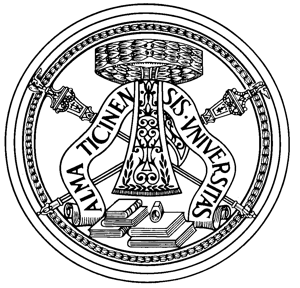
\includegraphics[width=2.5cm]{Figures/Unipv-logo}\\[.5cm] % Institution logo
\LARGE\institution\\ % Print institution name
\Large\emph{\department}\\[.1cm]

\large\course\\[.2cm] % Print department name
\normalsize % Degree or other information
\par
\hrulefill
\vfill}
\renewcommand{\maketitlehookb}{\vfill}

\renewcommand{\maketitlehookc}{
\vfill

\begin{flushleft}
Supervisore:\\
\textbf{Dott. Claudio Dappiaggi}\\[.3cm] % Advisor's/supervisor's name
Co-supervisore:\\
\textbf{Dott. Nicol\'o Drago}\\[.3cm] % Advisor's/supervisor's name
\end{flushleft}
\vfill}
\preauthor{%\LARGE $\Box u=\delta$\\
	\vfill\normalsize\begin{flushright} Relazione per la laurea di:\\\bfseries} % Text prior to the author name - right aligned and bold
\postauthor{\end{flushright}
} % After the author name, stop right alignment

%----------------------------------------------------------------------------------------

\makeindex % Write an index file

\begin{document}

\begin{titlingpage}
\maketitle % Print the title page
\end{titlingpage}

\thispagestyle{empty}

\bigskip\begin{quotation}\begin{center}\begin{em}
			
			\hfill A mamma e pap\`{a}
			
		\par\end{em}\end{center}\end{quotation}

\cleartoverso % Force a break to an even page


\thispagestyle{empty}
\begin{abstract}
	\noindent La tesi si propone di analizzare la risolubilit\'a di equazioni differenziali alle derivate parziali di tipo ondulatorio e le loro propriet\'a tramite la costruzione di soluzioni fondamentali distribuzionali. Dapprima si affronter\'a il caso nello spazio di Minkowski $n$-dimensionale e poi si trasporteranno, per quanto possibile, le principali propriet\'a delle soluzioni su particolari variet\'a curve di interesse per le loro applicazioni fisiche.\\

	\hfill
	
	\noindent The aim of the thesis is to analyse the solvability of wave-like partial differential equations and their properties via the construction of distributional fundamental solutions. Initially will be explored the $n$-dimensional Minkowski case and then the main properties of the solutions will be translated, when possible, on particular manifolds, interesting for their physical applications.
\end{abstract}

\cleartoverso % Force a break to an even page

\frontmatter % Use roman page numbering style (i, ii, iii, iv...) for the pre-content pages
%----------------------------------------------------------------------------------------
%	PREFACE
%----------------------------------------------------------------------------------------

%\section*{Introduzione}
%\textbf{To do}
%\begin{flushright}
%\textsc{\theauthor}\\
%Pavia\\
%July 2017
%\end{flushright}

%\cleartoverso % Force a break to an even page

%----------------------------------------------------------------------------------------
%	ABSTRACT
%----------------------------------------------------------------------------------------



%----------------------------------------------------------------------------------------
%	TABLE OF CONTENTS
%----------------------------------------------------------------------------------------

\tableofcontents* % Print the table of contents

\cleartoverso % Force a break to an even page


%----------------------------------------------------------------------------------------
%	CONTENT CHAPTERS
%----------------------------------------------------------------------------------------

\mainmatter % Begin numeric (1,2,3...) page numbering

\pagestyle{Ruled} % Include the chapter/section in the header along with a horizontal rule underneath

\chapterstyle{thesis2}
\chapter{Introduction}
\label{introduction}

\textit{Backflow} is an exotic quantum-mechanical phenomenon which can be heuristically depicted as a probability current associated to the quantum mechanical description of a particle moving on a line, flowing in the opposite direction with respect to the underlying momentum\footnote{see [\citealp[Abstract]{gand}]}.\\
In detail, we consider non-relativistic particles moving on a straight line. In \textit{quantum mechanics}, we describe the state of this particles at a given instant of time with a \textit{wave-function} $\psi\in L^2(\mR;\mC)$ where $|\psi(x)|^2$ represents the probability density of finding the particle in any open subset $I\subseteq\mR$. The time-evolution of such wave-functions $\psi(t)$ is ruled by the \textit{Schr\"{o}dinger equation}
\begin{equation}
	i\partial_t\psi(t)=H\psi(t)\, ,
\end{equation}
where $H$ is the \textit{Hamiltonian} which codifies the dynamics of the system. Here, for simplicity, we set all parameters and physical constants to $1$. Furthermore, we restrict ourselves to considering particles "travelling to the right". This statement can be formulated by requiring that the Fourier transform of this wave-function in \textit{momentum space} is supported only on $(0,+\infty)$. These wave-functions will be called \textit{right-movers}.\\
In this scenario, one might think that the probability density must flow to the right for all $t\in(0,+\infty)$ and everywhere in space. Hence the probability of finding the particle on the right of a given reference point might seem to be increasing with time. Counterintuitively, instead the probability can decrease in time. this phenomenon is referred to as \textit{quantum backflow}.\\
The scope of this work is to report and to discuss the main results regarding the fundamental properties as well as the magnitude of backflow in two different scenarios: the \textit{non-interacting} and the \textit{interacting} one.\\
For \textit{free particles}, we will prove that the amount of probability which can 
"flow back" through a reference point in a given interval of time is ruled by a suitable bounded and self-adjoint  $B$, called \textit{backflow operator}. Then, we will prove that the maximum amount of backflow $\lambda$ is equal to the supremum of the spectrum of $B$. We refer to $\lambda$ as \textit{backflow constant}. Using numerical methods, we will estimate $\lambda\approx0.038452$. We will also study the spatial extension of backflow using the density current $j_\psi(x)=i/2(\psi(x)\partial_x\psi^*(x)-\psi^*(x)\partial_x\psi(x))$. In detail, we will prove that there exists a constant $\beta_0(f)$ such that
\begin{equation}
	\int_{-\infty}^{\infty}\nspace f(x)j_\psi(x)\, \dd x \ge \beta_0(f)>-\infty
	\label{eq:first}
\end{equation}
for all normalized right-moving wave functions and for all positive averaging functions $f\ge0$.\\
In the \textit{interacting scenario}, we will investigate the presence of backflow for particles scattering against a potential wall $V$. Herein, complications arise since the presence of a potential $V$ implies the splitting of the incident wave-function into a transmitted and a reflected component which travel in opposite direction. This makes the concept of "right-moving" particle less clear. Hence we will introduce \textit{asymptotic} right-movers as those wave-functions that far away in the past, and far away from the potential wall $V$, behave like free and right-moving wave-functions. If we consider a non-interacting right-mover $\phi$, it might be seen as the incoming asymptotic form of an interacting state $\psi$. The link between the two wave-functions is given by the \textit{M\o{}ller operator} $\Omega_V$ of the Hamiltonian with the potential $V$, $\psi=\Omega_V\phi$. In this scattering scenario, our scope is to generalize the result (\ref{eq:first}). Stated differently, we shall study the existence of lower bounds for the average
\begin{equation}
	\int_{-\infty}^{\infty}\nspace\!f(x)j_{\Omega_V\psi}(x)\,\dd x
\end{equation}
for a generic normalized right-mover $\psi$ and for a positive function $f\ge0$. Although the reflection component can interfere, we will prove that there exists, for all short range potentials $V$ and for all positive smearing functions $f\ge0$, a constant $\beta_V(f)>-\infty$ such that
\begin{equation}
	\int_{-\infty}^{\infty}\nspace\!f(x)j_{\Omega_V\psi}(x)\,\dd x\ge\beta_V(f)
	\label{eq:second}
\end{equation}
for all normalized right-mover $\psi$.\\
 \\ 

The thesis is organized as follows.\\
In the first chapter, it will be presented an overview of the main mathematical
notions needed in order to set the discussion on quantum mechanics and backflow. The main
topics will be \textit{Hilbert spaces}, \textit{operators} and their \textit{spectrum}, \textit{Schwartz test-functions}, \textit{Fourier transform} as well as the basic concepts of quantum mechanics with particular attention both to the \textit{interacting picture} in scattering scenarios and to \textit{M\o{}ller operators}. \\
In the second chapter, it will be discussed the backflow effect in a non-interacting scenario. First of all, we will begin with an historical overview of the results obtained in the past concerning quantum backflow, from the first theoretical formulations, until the most recent analytical and numerical results. Then we introduce the problem of backflow for a free-particle. We will define rigorously the concept of \textit{right-mover} and give some examples of wave-functions in which backflow occurs. Then, we will search a lower bound for the flux of probability across a reference point in a given time interval. To do this, we must reformulate the problem as the search for an supremum of the spectrum of an operator called \textit{backflow operator}. We will prove that such a lower bound exists and hence that the flux of probability across the reference point is always greater than $-\lambda$, where $\lambda\in(0,1)$ is the \textit{backflow constant}. At the end of the chapter, numerical methods will be presented in order to estimate $\lambda$. In particular, using the \textit{power method} we will evaluate the backflow constant $\lambda\approx0.038452$.\\
The third chapter is divided in two main sections. In the first one, we will discuss the spatial extension of backflow for normalized right-movers at a given instant of time. It will be proved that the average of the density current for a right-moving state, as in (\ref{eq:first}), is bounded from below by a constant $\beta_0(f)\in(-\infty,0)$. The second section will be devoted to the analysis of backflow in scattering theory. First, the problem of backflow will be reformulated introducing the concept of \textit{asymptotic} right-moving wave-functions. Then, we will study the existence of a negative lower bound for the average current, as in (\ref{eq:second}). To do so, the infimum of the spectrum of an unbounded operator, called \textit{asymptotic current operator} will be investigated. At the end, we will prove that backflow can occur also in scattering scenarios and that the average current is always bigger than a suitable constant $\beta_V(f)$ determined by the potential $V$ and the positive smearing functions $f\ge0$. 
 % Include the introduction chapter

\chapterstyle{thesis} % Change the style of the Chapter header to that defined in structure.tex




\chapter{Mathematical Tools}
\label{chapter1}

\section{An overview of Differential Geometry}
We begin by recalling of very well known definitions in order to introduce the basic geometrical objects which are used in the text. In this section we will follow [\citealp{jost}] and [\citealp[Ch. A.3]{bar1}]\\
\noindent A \textbf{manifold} is, heuristically speaking, a space that is locally similar to $\mR^n$. To define it we use the concepts of \textbf{topological space} and of \textbf{homeomorphism}.
\begin{definition}[\textbf{Topological Space}]
	A set $\mathrm{X}$ together with a family $\mathcal{T}$ (\textbf{topology}) of subsets of $\mathrm{X}$ is called a \textbf{topological space} if the following conditions are met:
	\begin{enumerate}[label=\alph*. ]
		\item $\emptyset,\mathrm{X}\in\mathcal{T}$,
		\item for all $U$ and $V\in\mathcal{T}$, $U\cap V\in\mathcal{T}$,
		\item for any index set $A$, if $U_i\in\mathcal{T}$ for all $i\in A$, $\ds \bigcup_{i\in A} U_i\in\mathcal{T}$.
	\end{enumerate}
	An element of $\mathcal{T}$ is called \textbf{open set}. If a point $p$ is in an open set $U$, we call $U$ a \textbf{neighborhood} of $p$.
\end{definition}

\begin{definition}[\textbf{Continuity and homomorphism}]
	Let $\mathrm{X}$ and $\mathrm{Y}$ be two topological spaces. A function $f:\mathrm{X}\to\mathrm{Y}$ is \textbf{continuous} if for any open set $U$ of $\mathrm{Y}$, the preimage $f^{-1}(U)$ is an open set of $\mathrm{X}$.\\
	A continuous and bijective map $\varphi:\mathrm{X}\to\mathrm{Y}$ is an \textbf{homomorphism} if $\varphi^{-1}:\mathrm{Y}\to\mathrm{X}$ is also continuous.
\end{definition}
\noindent As for vector spaces, we can talk of a \textbf{basis} for topological space. A subset $\mathcal{B}\subset\mathcal{T}$ is a basis if any open set can be expressed as union of elements of $\mathcal{B}$.\\
A topology is \textbf{Hausdorff} if, for any two distinct points $p,q\in\mathrm{X}$, there exist two open neighborhoods $U$ of $p$ and $V$ of $q$ such that $U\cap V=\emptyset$.\\


\noindent A topological space $\mathrm{X}$ is called \textbf{compact} if each of its open covers has a finite subcover, i.e. for any collection $\{U_i\}_{i\in A}$, (where $A$ is a set of indexes) such that $$\mathrm{X}\subseteq\bigcup_{i\in A}U_i,$$ there is a finite subset $A'$ of $A$ such that $$ \mathrm{X}\subseteq\bigcup_{i\in A'}U_i.$$
The closure $\overline{\Omega}$ of a subset $\Omega\subset\mathrm{X}$ is the smallest closed set that contains $\Omega$. We say $\Omega$ is \textbf{relatively compact} if its closure $\overline{\Omega}$ is a compact subset.\\

\noindent We are now ready to introduce the concept of \textbf{manifold}.
\begin{definition}
	An $n$-dimensional topological \textbf{manifold} $\mathrm{M}$ is a topological Hausdorff space (with a countable basis) that is locally homeomorphic to $\mR^n$, i.e. for every $p\in\mM$ there exists an open neighbourhood $U$ of $p$ and a homeomorphism $$\varphi:U\to\varphi(U),$$ such that $\varphi(U)$ is an open subset of $\mR^n$.
\end{definition}
	
	\noindent Such homeomorphism is called a \textbf{(local) chart} of $\mM$. An \textbf{atlas} of $\mM$ is a family $\{U_i,\varphi_i\}_{i\in A}$ of local charts together with an open covering of $\mM$, i.e. $ \bigcup_{i\in A}U_i=\mM$.

	
\begin{figure}[h]
	\centering
	\begin{tikzpicture}[scale=1]
	\tikzstyle{every node}=[font=\scriptsize]
	\draw (0,0)  -- (10,0);
	\draw (0,0) -- (2,2);
	\node at (0.8,0.3) {$\mR^n$};
	
	\begin{scope}
	\clip (3,1.2) ellipse (1cm and 0.5cm);
	\draw [draw=black, fill=blue, opacity=0.4] (4,1.2) ellipse (1cm and 0.5cm);
	\end{scope}
	
	\begin{scope}
	\clip (8,1.2) ellipse (1cm and 0.5cm);
	\draw [draw=black, fill=blue, opacity=0.4] (7,1.2) ellipse (1cm and 0.5cm);
	\end{scope}
	
	\draw (3,1.2) ellipse (1cm and 0.5cm);
	\node at (3,0.4) {$\varphi_i(U_i) $};
	
	
	\draw [-latex] (5,3.5) to[out=-155,in=60] (3.2,1.9) node at (4,2.5) {$\varphi_i$};
	
	
	\draw (8,1.2) ellipse (1cm and 0.5cm);
	\node at (8,0.4) {$\varphi_j(U_j) $};
	
	\draw [-latex] (7,3.7) to[out=-40,in=100] (8,1.9) node at (8.2,2.5) {$\varphi_j$};
	
	
	\draw [ultra thin,-latex, color=blue] (4.2, 1.2) -- (6.8,1.2) node [pos=0.5,above] {$\varphi_i\circ\varphi_j^{-1}$};
	\draw (3,2.8) to[out=40,in=170] (9.5,5) node[below left] {$\mathrm{M}$} to[out=-100,in=50]  (7.5,2.8) to[out=170,in=20] (3,2.8);
	
	\node at (5.1,3.7) {$U_i$};
	\node at (7.1,4.5) {$U_j$};
	
	
	\begin{scope}
	\clip (6,4) ellipse (0.7cm and 0.5cm);
	\fill[blue, opacity=0.4, rotate around={-40:(6.2,4)}] (6.4,4) ellipse (0.6cm and 0.7cm);
	\end{scope}
	\draw [thin] (6,4) ellipse (0.7cm and 0.5cm);
	\draw [thin, rotate around={-40:(6.2,4)}] (6.4,4) ellipse (0.6cm and 0.7cm);
	
	\end{tikzpicture}
	\label{fig:atlas}
	\caption{A differentiable atlas on a manifold $\mM$.}
\end{figure}

\begin{definition}
	A \textbf{differentiable atlas} of a manifold $\mM$ is an atlas $\{U_i,\varphi_i\}_{i\in A}$ such that the functions
	$$\varphi_{ij}:=\textcolor{blue}{\varphi_i\circ\varphi_j^{-1}}:\varphi_j(U_i\cap U_j)\to\varphi_j(U_i\cap U_j),$$
	are differentiable (of class $C^\infty$) for any $i,j\in A$ such that $U_i\cap U_j\neq \emptyset$. Each $\varphi_{ij}$ is called \textbf{transition function}.
\end{definition}


	\noindent With this definition, each $\varphi_{ij}$ is a \textbf{diffeomorphism} because one can always interchange the indexes $i$ and $j$.\\



	\noindent We are only interested in \textbf{differentiable} (or \textbf{smooth}) \textbf{manifolds}, endowed with a maximal differentiable atlas. Here maximality of the atlas means that, if $\varphi$ is a chart of $\mM$ and $\{U_i,\varphi_i\}_{i\in A}$ is a differentiable atlas, then $\varphi$ belongs to $\{U_i,\varphi_i\}_{i\in A}$. We call a differentiable manifold with an atlas for which all chart transitions have positive Jacobian determinant an \textbf{orientable manifold}.
\begin{rem}
	For now on, the word \textbf{manifold} will always mean \textbf{differentiable manifold} and to indicate them it will be used the letters $\mM$ or $\mathrm{N}$.
\end{rem}


\begin{definition}[\textbf{Submanifold}]
	Let $n\leq m$. An $n$-dimensional \textbf{submanifold} $\mathrm{N}$ of $\mM$ is a nonempty subset $\mathrm{N}$ of $\mM$ such that, for every point $q\in\mathrm{N}$, there exists a local chart $\{U,\varphi\}$ of $\mM$ about $q$ such that
	$$\varphi(U\cap \mathrm{N})=\varphi(U)\cap(\mR^n\times\{0\})\subset\mR^m.$$ If $n=m-1$ we call $\mathrm{N}$ an \textbf{hypersurface} of $\mM$.
\end{definition}

\begin{example}
	If $\mM$ and $\mathrm{N}$ are manifolds, the Cartesian product $\mM\times\mathrm{N}$ is endowable with canonical structure of a manifold. If $\{U_i,\varphi_i\}_{i\in A}$ is an differentiable atlas for $\mM$ and $\{V_j,\psi_j\}_{j\in B}$ ia an atlas for $\mathrm{N}$, then $\big\{U_i\times V_j,(\varphi_i,\psi_j)\big\}_{(i,j)\in A\times B}$ is a differentiable atlas for $\mM\times\mathrm{N}$.
\end{example}

	\noindent As in the Euclidean case, one can introduce the notion of \textbf{differentiable} map between manifolds:
\begin{figure}[h]
	\centering
	\begin{tikzpicture}[scale=0.9]
	\tikzstyle{every node}=[font=\scriptsize]
	\draw (0,0)  -- (5,0);
	\draw (0,0) -- (2,2);
	\node at (0.8,0.3) {$\mR^n$};
	\draw (6,0)  -- (12,0);
	\draw (6,0) -- (8,2);
	\node at (6.8,0.3) {$\mR^m$};
	
	
	
	
	\draw [thin] (3,1.2) ellipse (1cm and 0.5cm);
	\node at (3,0.4) {$\varphi(U) $};
	
	
	\draw [-latex] (3.5,3.5) to[out=-110,in=90] (3.2,1.9) node at (3,2.5) {$\varphi$};
	
	
	\draw [thin] (10,1.2) ellipse (1cm and 0.5cm);
	\node at (10,0.4) {$\psi(V) $};
	
	\draw [-latex] (10,2.9) to[out=-70,in=80] (10,1.9) node at (10.3,2.3) {$\psi$};
	
	\draw [-latex] (4.8,4.2) to[out=10,in=150] (8.9,3.6);
	\node at (6.5,4.1) {$f$};
	
	
	\draw [ultra thin,-latex, color=red] (4.2, 1.2) -- (8.8,1.2) node [pos=0.5,above] {$\psi\circ f\circ\varphi^{-1}$};
	
	
	\draw (1,2.8) to[out=40,in=170] (7.5,5) node at (7,4.8) {$\mathrm{M}$} to[out=-100,in=50]  (5.5,2.8) to[out=170,in=20] (1,2.8);
	
	\node at (3.1,3.7) {$U$};
	
	\draw [thin] (4,4) ellipse (0.7cm and 0.5cm);
	\fill [black] (4,4) circle (0.05cm) node [right] {$p$};
	
	\node at (9.7,4.9) {$\mathrm{N}$};
	
	\begin{scope}[shift={(10.3,4.2)},scale=0.6]
	
	
	
	\draw (-3.5,0) .. controls (-3.5,2) and (-1.5,2.5) .. (0,2.5);
	\draw[xscale=-1] (-3.5,0) .. controls (-3.5,2) and (-1.5,2.5) .. (0,2.5);
	\draw[rotate=180] (-3.5,0) .. controls (-3.5,2) and (-1.5,2.5) .. (0,2.5);
	\draw[yscale=-1] (-3.5,0) .. controls (-3.5,2) and (-1.5,2.5) .. (0,2.5);
	
	\draw (-2,.2) .. controls (-1.5,-0.3) and (-1,-0.5) .. (0,-.5) .. controls (1,-0.5) and (1.5,-0.3) .. (2,0.2);
	
	\draw (-1.75,0) .. controls (-1.5,0.3) and (-1,0.5) .. (0,.5) .. controls (1,0.5) and (1.5,0.3) .. (1.75,0);
	\draw [thin, rotate around={-30:(-1.2,-1.3)}] (-1.2,-1.3) ellipse (1cm and 0.8cm);
	\fill [black] (-1.2,-1.3) circle (0.07cm) node at (-1.2,-0.93) {$f(p)$};
	\node at (0.1,-1.3) {$V$};
	\end{scope}
	
	
	
	
	\end{tikzpicture}
	\label{fig:diffmap}
	\caption{The notion of differentiable map $f$ between manifolds $\mM$ and $\mathrm{N}$.}
\end{figure}

\begin{definition}
	A continuous map $f:\mM\to\mathrm{N}$ between two manifolds $\mM$ and $\mathrm{N}$ is \textbf{differentiable} at $p\in\mM$ if there exist local charts $\{U,\varphi\}$ and $\{V,\psi\}$ about $p$ in $\mM$ and about $f(p)$ in $\mathrm{N}$ respectively, such that $f(U)\subset V$ and
	$$ \textcolor{red}{\psi\circ f\circ \varphi^{-1}}:\varphi(U)\to\psi(V),$$
	is differentiable (of class $C^\infty$) at $\varphi(p)$. The function $f$ is said to be differentiable on $\mM$ if it is differentiable at every point of $\mM$.
\end{definition}

	\noindent The space of differentiable functions between two manifolds is denoted by $C^\infty(\mM,\mathrm{N})$, and if $\mathrm{N}=\mC$ simply by $C^\infty(\mM)$. If $\psi\circ f\circ \varphi^{-1}$ is of class $C^k$, we say $f\in C^k(\mM,\mathrm{N})$.\\

	\noindent We introduce the \textbf{tangent space} of a point of a manifold. %It may be thought as a local approximation of the $\mR^n$ structure that lies on the manifold.
It will be constructed using the derivatives of curves which pass through the point. A tangent vector at a point $p$ is thought of as the velocity of a curve passing through the point. We can therefore define a tangent vector as an equivalence class of curves passing through $p$ while being tangent to each other at $p$.
.\begin{definition}[\textbf{Tangent space}]
	Let $p\in\mM$ and let $I$ be an interval containing $0$. We indicate $\mathcal{C}_p=\{c\in C^\infty(I,\mM)|\ c(0)=p\}$ the set of differentiable curves passing through $p$.\\
	We consider the equivalence relation ($\sim$), according to which two curves $c_1,c_2\in\mathcal{C}_p$ are equivalent if there exists a local chart $\varphi$ about $p$ such that $(\varphi\circ c_1)'(0)=(\varphi\circ c_2)'(0)$.\\
	The \textbf{tangent space} of $\mM$ at $p$ is the set
	$\mT_p\mM:=\mathcal{C}_p/\sim.$
\end{definition}

\noindent We will refer at the equivalence class of curves with $\dot{c}$, as they are uniquely determined by the velocity $(\varphi\circ c)'(0)$ at which they pass through the point $p$.


	\noindent One can check that the definition of the equivalence relation does not depend on the choice of local chart. In fact, if $\{U,\varphi\}$ and $\{V,\psi\}$ are local charts at $p$,
\[ (\varphi\circ c)'(0)=(\varphi\circ\psi^{-1}\circ\psi\circ c)'(0)=D(\varphi\circ\psi^{-1})(\psi(p))\cdot(\psi\circ c)'(0),\]
where $D(\varphi\circ\psi^{-1})(\psi(p))$ stands for the Jacobian of the transition function calculated at $\psi(p)$. It holds that $(\varphi\circ c_1)'(0)$ and $(\varphi\circ c_2)'(0)$ coincide if and only if $(\psi\circ c_1)'(0)$ and $(\psi\circ c_2)'(0)$ coincide.\\

\begin{figure}[h]
	\centering
	\begin{tikzpicture}[scale=1.2]
	\tikzstyle{every node}=[font=\scriptsize]
	
	\draw (1,2.8) to[out=40,in=170] (7.5,5) node at (7,4.8) {$\mathrm{M}$} to[out=-100,in=50]  (5.5,2.8) to[out=170,in=20] (1,2.8);
	
	\begin{scope}[shift={(0,0)},scale=1]
	\clip (2.2,3.5)-- (4.7,3.5) -- (5.7,4.5) -- (3.2,4.5) -- cycle;
	\draw [draw=black, fill=white] (2.2,3.5)-- (4.7,3.5) -- (5.7,4.5) -- (3.2,4.5) -- cycle;
	\draw [ultra thin, dashed] (1,2.8) to[out=40,in=170] (7.5,5) node at (7,4.8) {$\mathrm{M}$} to[out=-100,in=50]  (5.5,2.8) to[out=170,in=20] (1,2.8);
	
	\end{scope}
	\fill [black] (4,4) circle (0.05cm) node [left] {$p$};
	\node at (5.7,4) {$\mathrm{T}_p\mathrm{M}$};
	
	\draw [thin, dashed, color=red] (3.5,3.5) to[out=50,in=-140] (4,4) to[out=40,in=-165] (5.2,4.5);
	\begin{scope}[shift={(4,4)},scale=1]
	\draw [-latex, color=red] (0,0)-- (40:0.7cm);
	\end{scope}
	\node at (3.4,3.65) {$c_1$};
	
	\draw [thin, dashed, color=blue] (4.2,3.5) to[out=90,in=-50] (4,4) to[out=130,in=-20] (3.4,4.3);
	\begin{scope}[shift={(4,4)},scale=1]
	\draw [-latex, color=blue] (0,0)-- (130:0.5cm);
	\end{scope}
	\node at (4.45,3.65) {$c_2$};
	
	
	
	
	
	
	
	
	\end{tikzpicture}
	\label{fig:tangent}
	\caption{Tangent space $\mT_p\mM$ where $c_1\nsim c_2$.}
\end{figure}


	\noindent It can be proven that (for a fixed atlas $\varphi$ about $p$) the following map is a linear isomorphism between $\mT_p\mM$ and $\mR^n$:
$$\begin{aligned} \Theta_\varphi:\ \mT_p&\mM &\to\ &\mR^n,\\
							&\dot{c}&\mapsto \ & (\varphi\circ c)'(0).
   \end{aligned} $$
Hence we can think of $\mT_p\mM$ as being a copy of $\mR^n$ attached to the point $p$ on the manifold.\\
For reasons that we will make clear later, we denote the basis of $\mT_p\mM$ as
\[\left\{  \parz{ }{x^1}\Big|_p,\dots,\parz{ }{x^n}\Big|_p    \right\}.\]

	\noindent Collecting all tangent spaces, one builds the \textbf{tangent bundle} of a manifold $\mM$, defined as:
\[ \mT\mM=\bigsqcup_{p\in\mM} \mT_p\mM=\bigcup_{p\in\mM} \{p\}\times \mT_p\mM. \]



\begin{definition}
	Let $f:\mM\to\mathrm{N}$ be a differentiable map and let $p\in \mM$. The \textbf{differential} of $f$ at $p$ is the linear map
	\[\dd_p f:\mT_p\mM\to\mT_{f(p)}\mathrm{N},\quad \dot{c}\mapsto [f\circ c]\cong (f\circ c)'(0).   \]
	The \textbf{differential} of $f$ is the map $\dd f:\mT\mM\to\mT\mathrm{N}$ such that $\dd f|_{\mT_p\mM}=\dd_p f$.
\end{definition}


\begin{figure}[h]
	\centering
	\begin{tikzpicture}[scale=1]
	\tikzstyle{every node}=[font=\scriptsize]
	
	\draw (1,2.8) to[out=40,in=170] (7.5,5) node at (7,4.8) {$\mathrm{M}$} to[out=-100,in=50]  (5.5,2.8) to[out=170,in=20] (1,2.8);
	
	\begin{scope}[shift={(0,0)},scale=1]
	\clip (2.15,3.45)-- (4.75,3.45) -- (5.75,4.55) -- (3.15,4.55) -- cycle;
	\draw [draw=black, fill=white] (2.2,3.5)-- (4.7,3.5) -- (5.7,4.5) -- (3.2,4.5) -- cycle;
	\draw [ultra thin, dashed] (1,2.8) to[out=40,in=170] (7.5,5) node at (7,4.8) {$\mathrm{M}$} to[out=-100,in=50]  (5.5,2.8) to[out=170,in=20] (1,2.8);
	
	\end{scope}
	
	\fill [black] (4,4) circle (0.05cm) node [left] {$p$};
	\node at (5.4,3.6) {$\mathrm{T}_p\mathrm{M}$};
	
	\draw [thin, dashed, color=red] (3.5,3.5) to[out=50,in=-140] (4,4) to[out=40,in=-165] (5.2,4.5);
	\begin{scope}[shift={(4,4)},scale=1]
	\draw [-latex, color=red] (0,0)-- (40:0.7cm);
	\end{scope}
	\node at (3.4,3.65) {$c$};
	
	\begin{scope}[shift={(6.5,0)},scale=1]
	\draw (1,2.8) to[out=80,in=190] (7.5,5) node at (7,4.5) {$\mathrm{N}$} to[out=-100,in=60]  (6.5,2.8) to[out=200,in=-20] (1,2.8);
	\end{scope}
	
	\begin{scope}[shift={(6.5,-0.4)},scale=1, rotate around={10:(4,4)}]
	\node at (5.9,4) {$\mathrm{T}_{f(p)}\mathrm{N}$};
	\clip (2.15,3.45)-- (4.75,3.45) -- (5.75,4.55) -- (3.15,4.55) -- cycle;
	\draw [draw=black, fill=white] (2.2,3.5)-- (4.7,3.5) -- (5.7,4.5) -- (3.2,4.5) -- cycle;
	%\draw [ultra thin, dashed] (1,2.8) to[out=40,in=170] (7.5,5) node at (7,4.8) {$\mathrm{M}$} to[out=-100,in=50]  (5.5,2.8) to[out=170,in=20] (1,2.8);
	
	\draw [thin, dashed, color=blue] (4.2,3.5) to[out=90,in=-50] (4,4) to[out=130,in=-20] (3.4,4.3);
	
	
	\begin{scope}[shift={(4,4)},scale=1]
	\draw [-latex, color=blue] (0,0)-- (130:0.5cm);
	\end{scope}
	\node at (4.5,3.7) {$f\circ c$};
	
	\fill [black] (4,4) circle (0.05cm) node [below left] {$f(p)$};
	
	\end{scope}
	
	\draw [-latex] (5,2.9) to[out=-40,in=-150] (8.5,2.5);
	\node at (6.8,2.3) {$f$};
	\draw [-latex] (5.5,4.2) to[out=20,in=150] (9.3,3.6);
	\node at (7.9,4.5) {$d_p f$};
	
	
	
	
	\end{tikzpicture}
	\label{fig:differential}
	\caption{A scheme of a differential map.}
	
\end{figure}

	\noindent Given $\mM$ and a chart $\{U, \varphi\}$ near $p$, fix $X=\dot{c}\in\mT_p\mM$. If we identify $\mT_p\mR\cong\mR$, we can interpret the differential $\dd_p f(X)$ of a function $f\in C^\infty(\mM)$ at a point $p$ as the \textbf{derivative} in the direction of $X$:
\[	\partial_X f(p):=\dd_p f(X).	\]
A functional which is linear and follows Leibniz rule, such as $\partial_X:C^\infty(\mM)\to\mR$, is called a \textbf{derivation}. The set of all derivations at $p$ is denoted as $\operatorname{Der}_p$ and it is a vector space. The map $X\in\mT_p\mM\mapsto\partial_X$ is an isomorphism between $\mT_p\mM$ and $\operatorname{Der}_p$.\\
Define:
\[	\parz{ }{x^i}\Big|_p:C^\infty(\mM)\to\mR,\quad f\mapsto\parz{f}{x^i}\Big|_p=\partial_X f(p),	\]
where $X=\dot{c}$ and $c(t)=\varphi^{-1}(\varphi(p)+te_i)$ ($e_i$ is the $i$-th canonical basis vector).\\
Note that, from the definition of the differential, it holds
\[ \partial_X f(p)=(f\circ c)'(0)=\parz{(f\circ \varphi^{-1})}{x^i}\Big|_{\varphi(p)},\]
which shows that the object we defined can be seen as a partial derivative in the usual sense.\\
It can be shown that the set of derivations $\{\parz{ }{x^1},\dots,\parz{ }{x^n}\}$ forms a basis for $\operatorname{Der}_p$ and, due to the isomorphism, for $\mT_p\mM$, $X$ can be expressed as
\[	X=X^i\parz{ }{x^i},	\]
where Einstein summation has been employed.\\
Observe that linearity entails that
\[	\partial_X f(p)=\dd_p f(X)=X^i\dd_p f\left(\parz{}{x^i}\Big|_p\right)=X^i\parz{f}{x^i}\Big|_p.		\]

\begin{figure}
	\centering
	\[
	\begin{tikzcd}[column sep=1.5em]
	& \mT_p\mM \arrow{dr}{\Theta_\varphi} \\
	\operatorname{Der}_p \arrow[<-]{ur}{X\mapsto \partial_X} && \mR^n
	\end{tikzcd}
	\]
	\caption{Isomorphism relations for the tangent space.}
\end{figure}






\begin{definition}
	Let $\mM$ be a manifold, we define a projection map $\pi:\mT\mM\to\mM$ such that $\pi(\mT_p\mM)=p$, and we call a \textbf{section} in the tangent bundle a map $s:\mM\to\mT\mM$ such that
	$\pi\circ s=\operatorname{id}_\mM.$
\end{definition}
	\noindent The dual space of the tangent space $\mT_p\mM$ is called the \textbf{cotangent space}, denoted with $\mT^*_p\mM$, which has a canonical basis denoted with $\{\dd x^1|_p,\dots,\dd x^n|_p\}$.\\
	The elements of such basis act on any element of the tangent space basis at $p$ as follows:
	\[	\dd x^i|_p\left(\parz{}{x^j}\Big|_p\right)=\delta_{ij}.		\]
	Similarly is defined the \textbf{cotangent bundle} $\mT^*\mM$ as the disjoint union of cotangent spaces.
	\begin{definition}
	Sections in the tangent bundle, denoted by $C^\infty(\mM,\mT\mM)$, are called \textbf{vector fields}, whereby sections in the cotangent bundle are called \textbf{$1$-forms}.
	\end{definition}

	Vector fields are locally expressed in terms of linear combinations of \[\left\{  \parz{ }{x^1},\dots,\parz{ }{x^n}    \right\}=:\left\{\partial_1,\dots,\partial_n\right\},\] where $\partial_i=\partial_i|_p$ at any point $p$, whereas $1$-forms are expressed as linear combinations of $$\{\dd x^1,\dots,\dd x^n\},$$
	where $\dd x^i$ is the $1$-form that acts at $p$ as $\dd x^i|_p$.




\begin{definition}
We define the derivative in the direction of $X$ as an operator $\partial_X:C^\infty(\mM)\to C^\infty(\mM)$ such that
	\[ \partial_X f=\dd f(X), \]
for any vector field $X\in C^\infty(\mM,\mT\mM)$.
\end{definition}
\noindent It follows immediately that Leibniz's rule holds: $\ds \partial_X (f\cdot g)=g\,\partial_Xf +f\,\partial_X g$, and again holds the useful formula
\[	\partial_X f=\dd f(X)=X^i\dd f(\partial_i)=X^i\parz{f}{x^i}.	\]

\begin{oss}
	Given two vector fields $X,Y\in C^\infty(\mM,\mT\mM)$, there is a unique vector field $[X,Y]\in C^\infty(\mM,\mT\mM)$ such that
	\[		\partial_{[X,Y]}f=\partial_X\partial_Y-\partial_Y\partial_X f \]
	for all $f\in C^\infty(\mM)$. The map $[\cdot,\cdot ]:C^\infty(\mM,\mT\mM)\times C^\infty(\mM,\mT\mM)\to C^\infty(\mM,\mT\mM)$ is called the \textbf{Lie bracket}, it is bilinear, skew-symmetric and satisfies the \emph{Jacobi identity}: for any $X,Y,Z\in C^\infty(\mM,\mT\mM)$ holds
	\[	\left[[X,Y],Z\right]+\left[[Y,Z],X\right]+\left[[Z,X],Y\right]=0.		\]
\end{oss}

\begin{definition}
	An \textbf{affine connection} or \textbf{covariant derivative} on a manifold $\mM$ is a bilinear map
	
	\[\begin{split}
	\nabla: C^\infty(\mM,\mT\mM)\times C^\infty(\mM,\mT\mM) & \rightarrow C^\infty(\mM,\mT\mM)\\
	(X,Y) & \mapsto \nabla_X Y\,,
	\end{split} \]
	such that for all smooth functions $f\in C^\infty(\mM)$ and all vector fields $X,Y\in C^\infty(\mM,\mT\mM)$:
	\begin{itemize}
		\item 	$\nabla_{fX}Y= f\nabla_X Y$, i.e., $\nabla$ is $C^\infty(\mM)-$linear in the first variable;
		\item $\nabla_Xf=\partial_X f$;
		\item $\nabla_X (fY) = Y\partial_X f+ f\nabla_X Y$, i.e., $\nabla$ satisfies the \emph{Leibniz rule} in the second variable.
	\end{itemize}
\label{defn:connection}
\end{definition}

\noindent The covariant derivative on the direction of the basis vector fields $\left\{\partial_1,\dots,\partial_n\right\}$ is indicated
\[	\nabla_{j}:=\nabla_{\partial_j}.	\]



\noindent We are now ready to introduce metric structures on manifolds.

\section{Lorentzian Manifolds}

In this section we will follow the approach delineated in [\citealp{pfaffle}] and in [\citealp[Ch. 1]{bar2}]. We start in the simple case of \textbf{Minkowski spacetime}.

\begin{definition}
	Let $V$ be an $n$-dimensional vector space. A \textbf{Lorentzian scalar product} is a nondegenerate symmetric bilinear form $\left\langle\cdot,\cdot\right\rangle$ with signature $(-+\dots +)$, i.e. such that one can find a basis $\{e_1,\dots, e_n\}$ such that
	\[	\left\langle e_1,e_1 \right\rangle=-1,\quad \left\langle e_i,e_j \right\rangle=\delta_{ij}\ \text{  if } i,j>1.	\]
	\end{definition}
\noindent The \textbf{Minkowski product} $\scalar{x}{y}_0$, defined by the formula
\[	\scalar{x}{y}_0=\eta_{ik}x^iy^k=-x_1\,y_1+x_2\,y_2+\cdots+x_n\,y_n,	\] with $\eta:=\operatorname{diag}(-1,1,\dots,1,1)$ is the simplest example of Lorentzian scalar product on $\mR^n$. The $n$-dimensional Minkowski space, denoted by $\mathbb{M}^n$ is simply $\mR^n$ equipped with Minkowski product.
	\begin{figure}[h]
		\centering
		\begin{tikzpicture}[scale=1.2]
		\tikzstyle{every node}=[font=\scriptsize]
		\draw [white,postaction={decorate,decoration={text along path,text align=center,text={|\scriptsize|lightlike}}}] (-1,1.3) to [bend right=60]  (1,1.3);
		
		\begin{scope}
		\clip (-2,2.5)-- (2,2.5) -- (-2,-2.5) -- (2,-2.5) -- cycle;
		\draw [dashed] (-1,1.2) to [bend right=60]  (1,1.2);
		\draw [dashed] (-1,-0.55) to [bend right=60]  (1,-0.55);
		\end{scope}
		
		
		
		\draw [white,postaction={decorate,decoration={text along path,text align=center,text={|\scriptsize|lightlike} }}] (-1,-0.5) to [bend right=50]  (1,-0.5);
		
		
		\draw [ultra thin, -latex] (-3,-2.5) -- (-3,2.5) node [below right]{$t$};
		\draw (2,2.5)-- (-2,-2.5);
		\draw (-2,2.5)-- (2,-2.5);
		\draw (0,2.5) ellipse (2 and 0.3);
		
		\draw (2,-2.5) arc[x radius=2, y radius=0.3, start angle=0, end angle=-180];
		\draw [dashed] (2,-2.5) arc[x radius=2, y radius=0.3, start angle=0, end angle=180];
		
		
		\fill [black] (0,0) circle (0.05cm) node at (-0.1,0) [left] {$0$};
		\node at (2,1.9) {$I_+(0)$};
		\node at (2,-1.9) {$I_-(0)$};
		\node at (0,1.8) {timelike};
		\node at (0,-1.8) {timelike};
		\node at (-1.5,0) {spacelike};
		\node at (1.5,0) {spacelike};
		
		
		
		\end{tikzpicture}
		
		\label{fig:mink}
		\caption{Minkowski time orientation.}
	\end{figure}
	
\begin{definition} We call the \textbf{negative squared length} of a vector $X\in V$
	\[\gamma(X)=-\norm{X}^2:=-\scalar{X}{X}. \]
	A vector $X\in V\setminus\{0\}$ is called
\begin{itemize}
	\item  \textbf{timelike} if $\gamma(X)>0$,
	\item \textbf{lightlike} if $\gamma(X)=0$,
	\item \textbf{spacelike} if $\gamma(X)<0$ or $X=0$,
	\item \textbf{causal} if it is either timelike or lightlike.
	\end{itemize}
\label{defn:gamma}
	\end{definition}
\noindent 	This definition will mostly be used for tangent vectors, in case $V$ is the tangent space of a Lorentzian manifold at a point.\\
	For $n\geq 2$ the set of timelike vectors $I(0)$ consists of two connected components. A \textbf{time orientation} is the choice of one of these two components, that we call $I_+(0)$.

	\begin{definition}	We call
	\begin{itemize}
		\item $J_+(0):=\overline{I_+(0)}$ (elements are called \textbf{future-directed}),
		\item $C_+(0):=\partial I_+(0)$ (upper \textbf{light cone}),
		\item $I_-(0):=-I_+(0)$, $J_-(0):=-J_+(0)$ (elements are called \textbf{past-directed}),
		\item $C_-(0):=-C_+(0)$ (lower \textbf{light cone}).
	\end{itemize}
	\end{definition}

	


\begin{definition}
	A \textbf{metric} $g$ on a manifold $\mM$ is the assignment of a scalar product at each tangent space $$g:\mT_p\mM\times\mT_p\mM\to\mR$$ which depends smoothly on the base point $p$. We call it a \textbf{Riemannian metric} if the scalar product is pointwise positive definite, and a \textbf{Lorentzian metric} if it is a Lorentzian scalar product.\\
	A pair $(\mM,g)$, where $\mM$ is a manifold and $g$ is a Lorentzian (Riemannian) metric is called a \textbf{Lorentzian (Riemannian) manifold}.
\end{definition}
\noindent The request of smooth dependence on $p$ may be specified as follows: given any chart $\{U,\varphi=(x^1,\dots,x^n)\}$ about $p$, the functions $g_{ij}:\varphi(U)\to\mR$ defined by $g_{ij}=g(\parz{ }{x^i},\parz{ }{x^j})$, for any $i,j=1,\dots,n$ should be differentiable. With respect to these coordinates one writes
\[ g=\sum_{i,j} g_{ij}\,\dd x_i\otimes \dd x_j\equiv\sum_{i,j}g_{ij}\,\dd x_i\, \dd x_j. \]

The scalar product of two tangent vectors $v,w\in\mT_p\mM$, with coordinate chart $\varphi=(x^1,\dots x^n)$, such that $v=v^i\parz{ }{x^i}$, $w=w^j\parz{ }{x^j}$ is
\[ \langle v,w\rangle=g_{ij}(\varphi(p))v^iw^j.   \]
When the choice of the chart is clear we will often write, with abuse of notation $g_{ij}(p):=g_{ij}(\varphi(p))$. We will indicate $(g^{ij})_{i,j=1,\dots, n}=(g_{ij})^{-1}$.\\

\noindent The \textbf{negative squared length} of a tangent vector $X$ at $p\in\mM$ generalizes naturally as follows:
\begin{equation}
	\gamma(X)=-\langle X,X\rangle.
	\label{eq:gamma}
\end{equation}

\noindent From now on $\mM$ will always indicate a \textbf{Lorentzian manifold}.

\begin{definition}
		A vector field $X\in C^\infty (\mM,\mT\mM)$ is called timelike, spacelike, lightlike or causal, if $X (p)$ is timelike, spacelike, lightlike or causal, respectively, at every point $p\in\mM$.\\
		
		\noindent A differentiable curve $c : I\to\mM$ is called timelike, lightlike,
		spacelike, causal, future-directed or past-directed if $\dot{c}(t)\in\mT_{c(t)}\mM$ is, for all $t\in I$, timelike, lightlike, spacelike, causal,
		future-directed or past-directed, respectively.\\
		
		\noindent A Lorentzian manifold $\mM$ is called \textbf{time-oriented} if there exists a nowhere vanishing timelike vector field on $\mM$. If a manifold is time-oriented, we refer to it as \textbf{spacetime}.
\end{definition}


\begin{figure}[h]
\centering
	\begin{subfigure}{.5\textwidth}

	\begin{tikzpicture}[scale=0.9]
	\tikzstyle{every node}=[font=\scriptsize]
	
	\draw (1,2.8) to[out=40,in=170] (7.5,5) node at (7,4.8) {$\mathrm{M}$} to[out=-100,in=50]  (5.5,2.8) to[out=170,in=20] (1,2.8);
	
	\begin{scope}[shift={(0,0)},scale=1]
	\clip (2.2,3.4)-- (4.7,3.4) -- (5.7,4.6) -- (3.2,4.6) -- cycle;
	\draw [draw=black, thin, fill=white] (2.4,3.5)-- (4.4,3.5) -- (5.4,4.5) -- (3.4,4.5) -- cycle;
	\draw [ultra thin, dashed] (1,2.8) to[out=40,in=170] (7.5,5) node at (7,4.8) {$\mathrm{M}$} to[out=-100,in=50]  (5.5,2.8) to[out=170,in=20] (1,2.8);
	
	\draw [thin, color=blue, fill=blue, fill opacity=0.2] (3,3.5) -- (4,4) -- (4.2,3.5) ;
	
	\draw [thin, color=blue, fill=blue, fill opacity=0.2] (3.8,4.5) -- (4,4) -- (5,4.5);
	
	%\draw [thin, color=blue, fill=blue, fill opacity=0.2] (3,3.5) -- (5,4.5)-- (3.8,4.5) -- (4.2,3.5) -- (3.8,4.5);
	
	
	\end{scope}
	\fill [black] (4,4) circle (0.05cm) node [left] {$x$};
	\node at (5.3,4) {$\mathrm{T}_x\mathrm{M}$};
	
	\end{tikzpicture}
	\caption{A time-oriented tangent space.}
	\end{subfigure}

	\begin{subfigure}{.5\textwidth}

			\begin{tikzpicture}[scale=0.9]
		\tikzstyle{every node}=[font=\scriptsize]
		
		\draw (1,2.8) to[out=40,in=170] (7.5,5) node at (7,4.8) {$\mathrm{M}$} to[out=-100,in=50]  (5.5,2.8) to[out=170,in=20] (1,2.8);
		
	
	\begin{scope}[shift={(-0.5,0.25)},scale=1]
	
	
	\begin{scope}[shift={(1.5,1.5)},scale=0.5]
	\clip (2.2,3.4)-- (4.7,3.4) -- (5.7,4.6) -- (3.2,4.6) -- cycle;
	\draw [thin, color=blue, fill=blue, fill opacity=0.2] (3,3.5) -- (4,4) -- (4.2,3.5) ;
	\draw [thin, color=blue, fill=blue, fill opacity=0.2] (3.8,4.5) -- (4,4) -- (5,4.5);
	\begin{scope}[shift={(4,4)},scale=1]
	\draw [-latex, color=red] (-0.4,-0.4)-- (0.4,0.4);
	\end{scope}
	
	\end{scope}
	
	\begin{scope}[shift={(2.5,2)},scale=0.5, rotate around={-25:(4,4)}]
	\clip (2.2,3.4)-- (4.7,3.4) -- (5.7,4.6) -- (3.2,4.6) -- cycle;
	\draw [thin, color=blue, fill=blue, fill opacity=0.2] (3,3.5) -- (4,4) -- (4.2,3.5) ;
	\draw [thin, color=blue, fill=blue, fill opacity=0.2] (3.8,4.5) -- (4,4) -- (5,4.5);
	\begin{scope}[shift={(4,4)},scale=1]
	\draw [-latex, color=red] (-0.4,-0.4)-- (0.4,0.4);
	\end{scope}
	\end{scope}
	
	\begin{scope}[shift={(3.5,2.3)},scale=0.5, rotate around={-25:(4,4)}]
	\clip (2.2,3.4)-- (4.7,3.4) -- (5.7,4.6) -- (3.2,4.6) -- cycle;
	\draw [thin, color=blue, fill=blue, fill opacity=0.2] (3,3.5) -- (4,4) -- (4.2,3.5) ;
	\draw [thin, color=blue, fill=blue, fill opacity=0.2] (3.8,4.5) -- (4,4) -- (5,4.5);
	\begin{scope}[shift={(4,4)},scale=1]
	\draw [-latex, color=red] (-0.4,-0.4)-- (0.4,0.4);
	\end{scope}
	\end{scope}
	
	\draw [ dashed, color=black] (3.5,3.5) to[out=40,in=-150] (6,4.5);
	\end{scope}
	
	\begin{scope}[shift={(1,0)},scale=1]
	
	
	\begin{scope}[shift={(1.5,1.5)},scale=0.5]
	\clip (2.2,3.4)-- (4.7,3.4) -- (5.7,4.6) -- (3.2,4.6) -- cycle;
	\draw [thin, color=blue, fill=blue, fill opacity=0.2] (3,3.5) -- (4,4) -- (4.2,3.5) ;
	\draw [thin, color=blue, fill=blue, fill opacity=0.2] (3.8,4.5) -- (4,4) -- (5,4.5);
	\begin{scope}[shift={(4,4)},scale=1]
	\draw [-latex, color=red] (-0.4,-0.4)-- (0.4,0.4);
	\end{scope}
	
	\end{scope}
	
	\begin{scope}[shift={(2.5,2)},scale=0.5, rotate around={-25:(4,4)}]
	\clip (2.2,3.4)-- (4.7,3.4) -- (5.7,4.6) -- (3.2,4.6) -- cycle;
	\draw [thin, color=blue, fill=blue, fill opacity=0.2] (3,3.5) -- (4,4) -- (4.2,3.5) ;
	\draw [thin, color=blue, fill=blue, fill opacity=0.2] (3.8,4.5) -- (4,4) -- (5,4.5);
	\begin{scope}[shift={(4,4)},scale=1]
	\draw [-latex, color=red] (-0.4,-0.4)-- (0.4,0.4);
	\end{scope}
	\end{scope}
	
	\begin{scope}[shift={(3.5,2.3)},scale=0.5, rotate around={-25:(4,4)}]
	\clip (2.2,3.4)-- (4.7,3.4) -- (5.7,4.6) -- (3.2,4.6) -- cycle;
	\draw [thin, color=blue, fill=blue, fill opacity=0.2] (3,3.5) -- (4,4) -- (4.2,3.5) ;
	\draw [thin, color=blue, fill=blue, fill opacity=0.2] (3.8,4.5) -- (4,4) -- (5,4.5);
	\begin{scope}[shift={(4,4)},scale=1]
	\draw [-latex, color=red] (-0.4,-0.4)-- (0.4,0.4);
	\end{scope}
	\end{scope}
	
	\draw [ dashed, color=black] (3.5,3.5) to[out=40,in=-150] (6,4.5);
	\end{scope}
	\draw [ dashed, color=black] (3.5,3.5) to[out=40,in=-150] (6,4.5);
	\node at (3.3,3.3) {$X$};
		
		\end{tikzpicture}
	\caption{A time-oriented manifold together with field lines of a timelike vector field $X$.}
	\end{subfigure}
	\label{fig:timemanif}
	\caption{Time orientations.}
\end{figure}

The \textbf{causality relations} on $\mM$ are defined as follows. Let $p,q\in\mM$,
\begin{itemize}
	\item $p\ll q$ iff there exists a future-directed timelike curve from $p$ to $q$,
	\item $p< q$ iff there is a future-directed causal curve from $p$ to $q$,
	\item $p\le q$ iff $p<q$ or $p=q$.
\end{itemize}
\noindent The causality relation "$<$" is a strict weak ordering and the relation "$\le$" makes the manifold a partially ordered set.\\

\begin{definition}
	The \textbf{chronological future} of a point $x\in\mM$ is the set $I_+^M(x)$ of points that can be reached by future-directed \textsl{timelike} curves, i.e.
	\[		I_+^M(x)=\{y\in\mM\ |\ x<y\}.	\]
	The \textbf{causal future} $J_+^M(x)$ of a point $x\in\mM$ is the set of points that can be reached by future-directed \textsl{causal} curves from $x$, i.e.,
	\[	J_+^M(x)=\{y\in\mM\ |\ x\le y\}.	\]
	Given a subset $A\subset \mM$ the \textbf{chronological future} and the \textbf{causal future} of $A$ are respectively
	\[	I_+^M(A)=\bigcup_{x\in A}I_+^M(x),\qquad J_+^M(A)=\bigcup_{x\in A}J_+^M(x).	\]
	In a similar way, one defines the \textbf{chronological} and \textbf{causal pasts} of a point $x$ of a subset $A \subset \mM$ by replacing \textsl{future-directed curves} with \textsl{past directed curves}. They are denoted by $I_-^M (x), I_-^M (A), J_-^M (x)$, and $J_-^M (A)$, respectively. We will also use the notation $J^M (A) := J_-^M (A) \cup J_+^M (A)$.
\end{definition}
\noindent Any subset $\Omega$ of a spacetime $\mM$ is a spacetime itself, if one restricts the metric to $\Omega$. So $I_{\pm}^{\Omega}(x)$ and $J_{\pm}^{\Omega}(x)$ are well defined.
\begin{definition}
	A subset $\Omega\subset\mM$ of a spacetime is called \textbf{causally compatible} if for any point $x\in\Omega$ holds
	\[	J_{\pm}^{\Omega}(x)=J_{\pm}^{\mM}(x)\cap\Omega,		\]
	where it can be noted that the inclusion "$\subset$" always holds.
\end{definition}

\noindent The condition we defined means that taken two points in $\Omega$ that can be joined by a causal curve in $\mM$, there also exists a causal curve connecting them inside $\Omega$.\\

\begin{figure}[h]
	\centering\begin{tikzpicture}
	\tikzstyle{every node}=[font=\scriptsize]
	\draw [black] plot [smooth cycle] coordinates { (0,0) (1,1) (3,0) (1.5,-1)};
	\node at (1.5,0) {$A$};
	\begin{scope}[shift={(2.7,-0.42)},scale=1]
	\draw [color=red] (0,0) -- (45:3cm);
	\end{scope}
	
	\begin{scope}[shift={(2.9,0.13)},scale=1]
	\draw [color=blue] (0,0) -- (-45:2.5cm);
	\end{scope}
	
	\begin{scope}[shift={(0.25,-0.33)},scale=1]
	\draw [color=red] (0,0) -- (135:3cm);
	\end{scope}
	
	
	\begin{scope}[shift={(0.3,0.58)},scale=1]
	\draw [color=blue] (0,0) -- (-135:3cm);
	\end{scope}
	
	\node at (1.5,1.7) {$J_+^M(A)$};
	\node at (1.5,-1.7) {$J_-^M(A)$};
	%\draw [ultra thin, -latex] (-2.5,-2.5) -- (-2.5,2.5) node [below right]{$t$};
	\end{tikzpicture}
	\label{fig:causalfuturepast}
	\caption{Causal future $J_+^M$ and causal past $J_-^M$ of a subset $A\subset\mM$. }
\end{figure}


\noindent We now can introduce the concept of \textbf{geodesics} and \textbf{exponential map}.

\begin{definition}
	Let $c : [a,b]\to \mM$ be a curve on a Lorentzian manifold $\mM$. The
	length $L\dot{c}$ is defined by (with Einstein summation convention )
	\[ L\dot{c}=\int_{a}^{b} \sqrt{|g(\dot{c}(t),\dot{c}(t))|}\,d t=\int_{a}^{b} \sqrt{\left|g_{ik}(c(t)) \deri{x^i}{t}\deri{x^k}{t}\right|}\,d t,\]
	where $x^i(t):=(\varphi\circ c)^i(t)$ are the coordinates of the point $c(t)$ in a chart $\varphi$.\\
	Given $p,q\in\mM$, if $p\leq q$ we define the \textbf{time-separation} between $p$ and $q$ as
	\[\tau(p,q)=\sup\{L[c]\ |\ c \text{ is a future directed causal curve from }p\text{ to } q\}, \]
	and $0$ otherwise.\\
	A \textbf{geodesic} between two points $p,q\in\mM$ such that $p\leq q$, if it exists, is a curve $c$ such that $L[c]=\tau(p,q)$, i.e. the curve of maximum time-separation.
\end{definition}
\noindent The request on the geodesics implies that (in variational sense) $\delta L\dot{c}=0$. It can be demonstrated that the stationary problem for the functional $L\dot{c}$ is equivalent to $\delta E\dot{c}=0$ for the functional, called \textbf{energy}, defined by
\[		E\dot{c}=\frac{1}{2}\int_{a}^{b} {|g(\dot{c}(t),\dot{c}(t))|}\,d t.	\]
Since the Euler-Lagrange equations for a functional $I[c]=\int_{a}^{b} f(t,c(t),\dot{c}(t))\, dt$ read
\[		\deri{ }{t}\left(\parz{f}{\dot{x}^i}\right)-\parz{f}{x^i}=0,	\]
being $c=(x^1,\dots,x^n)$, then, in our case, setting $f(t,c,\dot{c})=g(\dot{c},\dot{c})$:
\[  \frac{\dd^2 x^i}{\dd t^2}-\Gamma_{jk}^i\deri{x^j}{t}\deri{x^k}{t}=0.	\]
Here $\Gamma_{jk}^i\in C^\infty (U\subset\mM)$ are the \textbf{Christoffel symbols}, defined in the chart $\varphi=(\xi^1,\dots,\xi^n)$ as
\[	\Gamma_{jk}^i=\frac12 \sum_l g^{il} \left(
\frac{\partial g_{lj}}{\partial \xi^k} 
+\frac{\partial g_{lk}}{\partial \xi^j}
-\frac{\partial g_{jk}}{\partial \xi^l}
\right).	\]

\begin{definition}
	A connection $\nabla$ on a manifold $\mM$ with a metric $g$ is said to be a \textbf{metric connection} if for all $X,Y,Z\in C^\infty (\mM,\mT\mM)$ holds the following \emph{Leibniz rule}:
	\[		\partial_X\,g(Y,Z)=g(\nabla_X Y, Z)+g(Y,\nabla_X Z).	\]
	The unique metric connection which is also torsion-free, i.e.,
	\[		T:=\nabla_X Y-\nabla_Y X-[X,Y]=0,	\]
	is called the \textbf{Levi-Civita connection}. 
\end{definition}

\noindent Another way to define \textbf{geodesics} is to say a geodesic between two points $p,q$ on a manifold $\mM$ with the Levi-Civita connection $\nabla$ is the curve $c$ which links $p$ and $q$ such that parallel transport along it preserves the tangent vector to the curve, i.e.
\begin{equation}
	\nabla_{\dot{c}(t)}\dot{c}(t)=0\quad \text{for all } t\in [a,b].
	\label{eq:LCgeodesic}
\end{equation}
More precisely, in order to define the covariant derivative of $\displaystyle \dot{c}$ it is necessary first to extend $\displaystyle \dot{c}$ to a smooth vector field in an open set containing the image of the curve, but it can be shown that the derivative is independent of the choice of the extension.\\

\begin{oss}
	We can express the Christoffel symbols in terms of the Levi-Civita connection:
	\begin{equation}
			\nabla_{j}\partial_k=\Gamma_{jk}^i \partial_i
			\label{eq:LCchrist}
	\end{equation}
in a local chart $\varphi=(x^1,\dots,x^n)$.
\end{oss}

\begin{prop}
	Let $\nabla$ be a connection over a manifold $\mM$ and $X,Y\in C^\infty(\mM,\mT\mM)$ be vector fields. It holds
	\[	\nabla_X Y=\left(X^j\partial_jY^k+X^jY^i\Gamma_{ij}^k\right)\partial_k,		\]
	in particular
	\[	(\nabla_j Y)^i=\partial_jY^i+Y^i\Gamma_{ij}^k.		\]
\end{prop}
\Proof From Definition \ref{defn:connection} holds:
\[	\nabla_X Y=\nabla_{X^je_j}Y^i e_i=X^j\partial_j Y^i e_i=X^jY^i\nabla_j e_i+X^j e_i\partial_j Y^i=		\]
\[	=X^jY^i\Gamma_{ij}^k e_k+(X^j\partial_jY^k) e_k	.	\]


\begin{prop}
	Let us consider $p\in\mM$ and a tangent vector $\xi\in \mT_p\mM$. Then there exists $\epsilon>0$ and precisely one geodesic $$c_\xi:[0,\epsilon]\to\mM,$$ such that $c_\xi(0)=p$ and $\dot c_\xi(0)=\xi$.
\end{prop}

\begin{definition}
	In the conditions of the proposition above, if we put
	\[		\mathcal{D}_p=\{	\xi\in\mT_p\mM\ |\ c_\xi \text{ is defined on } [0,1]	\}\subset \mT_p\mM,	\]
	the \textbf{exponential map} at point $p$ is defined as $\exp_p:\mathcal{D}_p\to\mM$ such that $\exp_p(\xi)=c_\xi(1)$.\\
	The local coordinates defined by the chart $\{U:=\exp_p(\mathcal{D}_p),\exp_p^{-1} \}$ are called \textbf{normal coordinates} centered at $p$.
\end{definition}

\begin{figure}[h]
	\centering
		\begin{tikzpicture}[scale=1.3]
	\tikzstyle{every node}=[font=\scriptsize]
	
	\draw (1,2.8) to[out=40,in=170] (7.5,5) node at (7,4.8) {$\mathrm{M}$} to[out=-100,in=50]  (5.5,2.8) to[out=170,in=20] (1,2.8);
	
	\begin{scope}[shift={(0,2.5)},scale=1]
		\node at (5.4,3.6) {$\mathrm{T}_p\mathrm{M}$};
	%\clip (2.2,3.6)-- (4.7,3.5) -- (5.7,4.5) -- (3.2,4.5) -- cycle;
	\draw [draw=black, fill=white] (2.2,3.5)-- (4.7,3.5) -- (5.7,4.5) -- (3.2,4.5) -- cycle;
	\fill [black] (4,4) circle (0.03cm) node [left] {$0$};
	\draw [draw=blue, rotate around={0:(4,4)}] (4,4) ellipse (0.75cm and 0.45cm);
	
	\end{scope}
	
	\begin{scope}[shift={(4,6.5)},scale=1]
	\clip (0,0) ellipse (0.75cm and 0.45cm);
	\foreach \x in {0,...,9}
	\draw [thin, color=red] (0,0)-- ({5+40*\x}:2cm);
	\end{scope}
	
	
	\draw [ dashed] (4,6.5) -- (4,6);
	\draw [ -latex] (4,6) -- (4,4) node [pos=0.4, right] {$\exp_p$};
	
	
	\begin{scope}[shift={(0,0)},scale=1]
	%\clip (2.2,3.6)-- (4.7,3.5) -- (5.7,4.5) -- (3.2,4.5) -- cycle;
	\fill [black] (4,4) circle (0.03cm) node [left] {$p$};
	\draw [draw=blue, rotate around={0:(4,4)}] (4.15,4) ellipse (0.75cm and 0.45cm);
	
	\end{scope}
	
	\begin{scope}[shift={(4,4)},scale=1]
	\clip (0.15,0) ellipse (0.75cm and 0.45cm);
	\foreach \x in {0,...,4}
	\draw [thin, color=red] (0,0) to [bend right=60] ({5+40*\x}:2cm);
	\foreach \x in {4,...,6}
	\draw [thin, color=red] (0,0) to [bend left=40] ({5+40*\x}:2cm);
	\end{scope}
	
	
	\end{tikzpicture}
	\label{fig:exp}
	\caption{The exponential maps from the tangent space to the manifold.}
\end{figure}

\begin{prop}
	Given normal coordinates centered at $p\in\mM$, it holds
	\[	g_{ij}(p):=g_{ij}(\exp_p(0))=\eta_{ij},\] \[ \Gamma_{jk}^i=0,	\]
	for all indexes $i,j,k$.
\end{prop}

\noindent We are now ready to talk about \textbf{geodesically starshaped} sets.


\begin{definition}
	An open subset $\Omega\subset\mM$ is called \textbf{geodesically starshaped} with respect to a point $p\in\mM$ if there exists an open subset $\Omega'\subset\mT_p\mM$, starshaped with respect to 0, such that the exponential map
	\[	\exp_p|_{\Omega'}:\Omega'\to\Omega,		\]
	is a diffeomorphism. If $\Omega$ is geodesically starshaped with respect to all of its points, one calls it \textbf{convex}.
\end{definition}

\begin{prop}
	Under the conditions of the last definition, let $\Omega\subset\mM$ be geodesically starshaped with respect to point $p\in\mM$. Then one has
	\[	I_{\pm}^\Omega(p)=\exp_p(I_{\pm}(0)\cap\Omega'),		\]
	\[	J_{\pm}^\Omega(p)=\exp_p(J_{\pm}(0)\cap\Omega').		\]
\end{prop}

\noindent We continue our preparations with another function that we are going to need in Chapter (3).

\begin{definition}
	Let $\Omega\subset\mM$ be open and geodesically starshaped with respect to $x\in\Omega$. We define 
	\[	\Gamma_x:=\gamma\circ\exp_x^{-1}:\Omega\to\mR,		\]
	where $\gamma:\mT_x\mM\to\mR$ is defined in equation (\ref{eq:gamma}).
	\label{defn:Gamma}
\end{definition}


\subsection{Causality and Global Hyperbolicity}



Now we introduce causal domains, because they will appear in the theory of wave equations. The local construction of fundamental solutions is always possible on causal domains, provided they are small enough.


\begin{definition}
	A domain $\Omega\subset\mM$ is called \textbf{causal} if its closure $\overline{\Omega}$ is contained in a convex domain $\Omega'$ and for any $p,q\in\overline{\Omega}$ $J_{+}^{\Omega'}(p)\cap J_{-}^{\Omega'}(q)$ is compact and contained in $\overline{\Omega}$.\\
	A subset $A\subset\mM$ is called \textbf{past-compact} (respectively \textbf{future-compact}) if, for all $p\in\mM$, $A\cap J_-^{\mM}(p)$ (respectively $A\cap J_+^{\mM}(p)$) is compact.
	\label{defn:pastcompact}
\end{definition}

\begin{figure}[h]
	\centering
	\begin{tikzpicture}
	\draw[thin] (0,0) ellipse (2.5 and 2);
	\draw[thick] (0,0) ellipse (1 and 1.7);
	\fill [black] (0,1.25) circle (0.05cm) node [above] {$q$};
	\fill [black] (0,-1.25) circle (0.05cm) node [below] {$p$};
	\begin{scope}[shift={(0,-1.25)},scale=1]
	\draw (0,0) -- (1.5,1.5);
	\draw (0,0) -- (-1.5,1.5);
	\clip (0,0) -- (1.25,1.25) -- (0,2.5) -- (-1.25,1.25) -- cycle;
	\draw [thin, color=blue, fill=blue, fill opacity=0.2] (0,0) -- (1.25,1.25) -- (0,2.5) -- (-1.25,1.25) -- cycle;
	\end{scope}
	\begin{scope}[shift={(0,1.25)},scale=1]
	\draw (0,0) -- (1.5,-1.5);
	\draw (0,0) -- (-1.5,-1.5);
	\end{scope}
	\node at (1,1.25) {$\Omega$};
	\node at (-1.5,1.25) {$\Omega'$};
	\end{tikzpicture}
	\caption{Convex, but non causal, domain}
\end{figure}

\noindent We can notice that, if we look at compact spacetimes, something physically unsound occurs: 

\begin{prop}
	If a spacetime $\mM$ is compact, there exists a closed timelike curve in $\mM$.
	\label{prop:paradoxes}
\end{prop}
\noindent In a few words, there are manifolds, such as compact spacetimes, where there are timelike loops that can produce science fictional paradoxes. To avoid such unphysical and unrealistic things we require suitable causality conditions:
\begin{definition}
	A spacetime satisfies the \textbf{causality condition} if it does not contain any closed causal curve. A spacetime $\mM$ satisfies the \textbf{strong causality condition} if there are no almost closed causal curves, i.e. if for any $p\in\mM$ there exists a neighborhood $U$ of $p$ such that there exists no timelike curve that passes through $U$ more than once.
\end{definition}
\noindent It is clear that the strong causality condition implies the causality condition.
\begin{figure}
	\centering
	\begin{tikzpicture}
	\draw[thin] (0,0) ellipse (2.5 and 2);
	\draw[thick] (0,0) ellipse (1.7 and 1.43);
	\fill [black] (0,1) circle (0.05cm) node [above] {$q$};
	\fill [black] (0,-1) circle (0.05cm) node [below] {$p$};
	\begin{scope}[shift={(0,-1)},scale=1]
	\draw (0,0) -- (1.1,1.1);
	\draw (0,0) -- (-1.1,1.1);
	\clip (0,0) -- (1,1) -- (0,2) -- (-1,1) -- cycle;
	\draw [thin, color=blue, fill=blue, fill opacity=0.2] (0,0) -- (1,1) -- (0,2) -- (-1,1) -- cycle;
	\end{scope}
	\begin{scope}[shift={(0,1)},scale=1]
	\draw (0,0) -- (1.1,-1.1);
	\draw (0,0) -- (-1.1,-1.1);
	\end{scope}
	\node at (0.75,1) {$\Omega$};
	\node at (-2.5,1.25) {$\Omega'$};
	\end{tikzpicture}
	\caption{Causal domain}
\end{figure}
\begin{definition}
	A spacetime $\mM$ that satisfies the strong causality condition and such that for all $p,q\in\mM$ $J_+^{\mM}(p)\cap J_-^{\mM}(q)$ is compact is called \textbf{globally hyperbolic}.
	\label{defn:globalhyp}
\end{definition}

\noindent It can be demonstrated that in globally hyperbolic manifolds for any $p\in\mM$ and any compact set $K\subset\mM$ the sets $J_{\pm}^{\mM}(p)$ and $J_{\pm}^{\mM}(K)$ are closed.

\begin{definition}
	A subset $S$ of a connected time-oriented Lorentzian manifold $\mM$ is a \textbf{Cauchy hypersurface} if each inextensible timelike curve (i.e. no reparametrisation of the curve can be continuously extended) in $\mM$ meets $S$ at exactly one point.
	\label{defn:Cauchyhyper}
\end{definition}


\begin{figure}
	\begin{subfigure}{.5\textwidth}
	\begin{tikzpicture}
	\draw[thick] (-2,2) to[out=-30,in=105] (0,0) to[out=-75,in=190] (2,-0.5);
	\draw (0,0) -- (1.1,1.1);
	\draw (0,0) -- (-1.1,1.1);
	\draw (0,1.1) ellipse (1.1 and 0.18);
	\draw[fill=black] (0,0) circle (0.03cm);
	\node at (-1.7,0.6) {$S$};
	\end{tikzpicture}
	\caption{A non-Cauchy hypersurface}
\end{subfigure}
\begin{subfigure}{.5\textwidth}
	\begin{tikzpicture}
	\draw[thick] (-2,1) to[out=-20,in=140] (0,0) to[out=-40,in=190] (2,-0.5);
	\draw (0,0) -- (1.1,1.1);
	\draw (0,0) -- (-1.1,1.1);
	\draw (0,1.1) ellipse (1.1 and 0.18);
	\draw[fill=black] (0,0) circle (0.03cm);
	\node at (-1.7,0.6) {$S$};
	\end{tikzpicture}
	\caption{A Cauchy hypersurface}
\end{subfigure}
\caption{Hypersurfaces.}
\end{figure}


\noindent In other words, no point of a Cauchy hypersurface is in the light cone of another point of the surface.
\begin{theorem}
	Let $\mM$ be a connected time-oriented Lorentzian manifold. Then the following are equivalent:
	\begin{itemize}
		\item $\mM$ is globally hyperbolic.
		\item There exists a Cauchy hypersurface in $\mM$.
		\item $\mM$ is isometric to $\mR\times S$ with metric $g=-\beta\dd t^2+b_t$, where $\beta$ is a smooth positive function, $b_t$ is a Riemannian metric on $S$ depending smoothly on $t$ and each $\{t\}\times S$ is a smooth Cauchy hypersurface in $\mM$.
	\end{itemize}
	In such case there exists a smooth function $h:\mM\to\mR$ whose gradient is past-directed timelike at every point and all of whose level sets are Cauchy hypersurfaces.
	\label{th:Bernal}
\end{theorem}
\noindent We briefly give some examples of globally hyperbolic spacetimes.
\begin{example}
	The Minkowski spacetime $\mathbb{M}^n$ is globally hyperbolic. Every
	spacelike hyperplane is a Cauchy hypersurface. We have $\mathbb{M}^n=\mR\times S$ with $S = \mR^{n-1}$ , endowed	with the time-independent Euclidean metric.\\
	
\noindent	Let $S$ be a Riemannian manifold with time independent metric $b_t$ and $I\subset\mR$ an interval. Let $f: I\to\mR$
	be a smooth positive function. The manifold $\mM=I \times S$ with the metric $g = -\dd t^2 + f^2(t)\, b_t$, called \textbf{cosmological spacetime},
	is globally hyperbolic if and only if $S$ is a complete space, see [\citealp[Lem A.5.14]{bar1}]. This applies in particular if $S$ is compact.\\
	
	\noindent The interior and exterior \textbf{Schwartzschild spacetimes}, that represent non-rotating black holes of mass $m>0$ are globally hyperbolic.\\
	Denoting $S^2$ the $2$-dimensional sphere embedded in $\mR^3$, we set
	\[	\mM_{\text{ext}}:=\mR\times(2m,+\infty)	\times S^2,	\] 
	
	\[	\mM_{\text{int}}:=\mR\times(0,2m)	\times S^2.	\] 
	The metric is given by
	\[	g=-h(r)\dd t^2+\frac{1}{h(r)}\dd r^2	+r^2\,g_{S^2},	\]
	where $h(r)=1-\frac{2m}{r}$, while $g_{S^2}=r^2\,\dd\theta^2+r^2\sin^2\theta\dd\varphi^2$ is the polar coordinates metric on the sphere. For the exterior Schwartzschild spacetime we have $\mM_{\text{ext}}=\mR\times S$ with $S=(2m,+\infty)\times S^2$, $\beta=h$ and $b_t=\frac{1}{h(r)}\dd r^2	+r^2\,g_{S^2}$.
	\label{ex:spacetimes}
\end{example}




\section{Operators and integration on manifolds}
\label{sec:operators}
We call $C_0^\infty(\mM)$ the set of $C^\infty$ functions on a manifold with compact support. The integral map\footnote{see [\citealp[Ch. A.3]{bar1}]} is defined as the unique map
\[	\int_{\mM}\cdot\ \dd\mu:C_0^\infty(\mM)\to \mC,	\]
such that it is linear and for any local chart $\{U,\varphi\}$ and for any $f\in C_0^\infty(U)$ holds
\[	\int_{\mM}f\,\dd\mu=\int_{\varphi(U)}(f\circ\varphi^{-1})(x)\,\mu_x\,\dd x,		\]
where we define \begin{equation}
	\mu_x:=|\det g(x)|^{1/2}.
	\label{eq:mu}
\end{equation}

\noindent In this section we introduce the \textbf{generalized d'Alembert} operators, whose general form in local coordinates is given by
\begin{equation}
	P=-g^{ij}(x)\frac{\partial^2}{\partial x^i\partial x^j}+a_j(x)\parz{}{x^j}+b(x).
%	\label{eq:generalizedAlembert}
\end{equation}
The d'Alembert wave operator $\Box$ is defined for smooth functions $f$ as
\[	\Box f=-\operatorname{div}\grad f,	\]
where $\grad f$ is a vector field defined by the requirement that the formula $$\scalar{\grad f}{X}=\partial_X f$$ holds for any vector field $X$. At the same time $\operatorname{div}$ is defined as follows
\begin{definition}
	The \textbf{divergence} of a vector field $Z=Z^i\partial_i$ is defined as
	\[	\operatorname{div}Z=\sum_{j}(\nabla_j Z)_j=\partial_jZ^j+\Gamma_{ij}^iZ^j.	\]
\end{definition}

\begin{prop}
	The following formula holds:
	\begin{equation}
		\operatorname{div}Z=\mu_x^{-1}\parz{}{x^j}\left(\mu_xZ^j\right),
		\label{eq:divergence}
	\end{equation}
		
\noindent 	and the definition of divergence is consistent with that of integral.
\end{prop}
\Proof Let $h\in C_0^\infty(\mM)$; using integration by parts
\[	\int_{\mM} h\cdot\operatorname{div}(Z)\dd\mu=-\int_\mM Z^j \partial_j h\,\dd\mu = -\int_\mM Z^j \partial_j h\, \mu_x\,\dd x.	\]
Now integrating by parts again in the chart it holds:
\[	-\int_\mM \partial_j h\  Z^j \mu_x\, \dd x= \int_\mM h\ \partial_j (\mu_x\, Z^j)\, \dd x = \int_\mM h\ \mu_x^{-1}\partial_j(\mu_x\ Z^j)\, \dd\mu.		\]
Since this is true for any function $h$, the formula is proven.\endproof\\

\noindent From the definition of gradient one can show
\[g_{ij}(\grad f)^iX^j=\partial_X f=X^j\parz{f}{x^j},\quad \grad f=g^{ij}\parz{f}{x^i}\partial_j.\]
Hence it holds
\[	\Box f=-\mu_x^{-1}\parz{}{x^j}\left(\mu_x\, g^{ij}\parz{f}{x^i}\right).	\]
In Minkowski spacetime, where $g=\eta$,
\[	\Box f=-\parz{}{x^j}\left(\eta^{jj}\parz{f}{x^j}\right)=\frac{\partial^2f}{\partial t^2}-\sum_{i=1}^{n-1}\frac{\partial^2f}{\partial x_i^2}=-\partial^i\partial_if.		\]


 % Include the first content chapter
\chapter{Quantum Backflow - Basic Concepts}
%[\citealp[Ch. 2]{bar2}]
\label{chapter2}

In this chapter we start our discussion on the backflow effect. First of all, we will give an historical introduction on the first observations and subsequently we dwell into a deeper analysis. Then, we will give a rigorous definition of backflow reporting a few illustrative and relevant examples. In the central part of this chapter we will focus on outlining the basic properties of backflow in free field theories. For this purpose, we shall retrace the first work of Braken and Melloy [\citealp{bracken}], outlining its most important results and discussing in detail and rigorously their results.\\
As we remarked in Section \ref{sec:quantum_mechanincs}, considering particles of mass $m>0$, it will be convenient to work with dimensionless variables for position $x$, momentum $p$, etc., and dimensionless functions (such as the wave function $\psi$ and the current $j_\psi$) by using a length scale $\ell$ as the unit of length, $\hbar/\ell$ as the unit of momentum, $m\ell^2/\hbar$ as the unit of time, and $\hbar^2/m\ell^2$ as the unit of energy, effectively setting $m=\hbar=1$.



 %The most outstanding property that we will prove is the temporal boundedness of backflow through some point during a certain interval of time and the independence of this bound from the external parameter such as the mass of the particle and the length of the time interval. Considering particles of mass $m>0$, it will be convenient to work with dimensionless variables $x$, $p$, etc., and dimensionless functions (such as the wave function $\psi$ and the current $j_\psi$) by using a length scale $\ell$ as the unit of length, $\hbar/\ell$ as the unit of momentum, $m\ell^2/\hbar$ as the unit of time, and $\hbar^2/m\ell^2$ as the unit of energy, effectively setting $m=\hbar=1$.

\section{Historical Introduction}
Let us start by contextualizing the problem from which quantum backflow arises. Consider a particle bounded to travel freely on a straight line. According to Section \ref{sec:quantum_mechanincs}, all particles are described by a wave function $\psi(x,t)$ whose square of absolute value $|\psi(x,t)|^2$ gives the probability density of finding the particle at some point of space $x$ and at some time $t$. At the same time, if we take the Fourier transform, $\hat{\psi}(p,t)$, its square of absolute value $|\hat{\psi}(p,t)|^2$ gives the density probability of finding the particle with a given momentum $p$.\\
Suppose to shoot such a quantum particle with a given positive velocity along the straight line. Hence $\hat{\psi}(p)\neq 0$ only if $p>0$. Now consider the probability $P(t)$ of finding the particle behind a certain point, say for definiteness the origin $x=0$, at a given time $t$:
\begin{equation}
	P(t):=\int_{-\infty}^{0}\nspace\!|\psi(x,t)|^2\, \dd x
\end{equation}
Consider the following question:
\begin{verse}
	\centering
	\emph{For each wave function with strictly positive momentum, is the quantity $P(t)$ always decreasing over time?}
	\end{verse}
Classically, the answer is obvious. If you consider a particle with positive velocity, its position certainly increases with time. Instead in Quantum Mechanics, the outcome is more exotic and wave functions with positive velocity, but increasing $P(t)$ exist. This is \textit{quantum backflow}.\\
First analysis of this phenomenon date back to 1969 in a work written by Allcock [\citealp{allcock}] on the problem of time arrival as a physical observable in quantum mechanics. After that, backflow has been neglected until 1994, when Bracken and Melloy made an exhaustive investigation outlining the fundamental properties and quantitative bounds in free theory. Subsequently, Eveson, Fewster and Verch [\citealp{verch}] described backflow as a fundamental quantum inequality and in 2013 Palmero [\citealp{palmero}] gave suggestion for an experimental observation using Bose-Einstein condensate. The analysis of the results obtained by Bracken and Melloy will be discussed in this chapter while the next one will discuss mainly the study of backflow in scattering theory (particles subjected to a potential) treated in the recent work of Bostelmann, Cadamuro and Lechner [\citealp{gand}].


\section{Definition of Backflow and Illustrative Examples}
\label{sec:examples1}

The first goal of this section is to give a complete set of definitions in order to clarify the nature of backflow and the mathematics the lies behind it. We start by clarifying our notion of particles with only positive momentum by introducing the concept of \textit{right-movers}.

\begin{definition}[\textbf{Right-mover}]
	\label{def:right-mover}
	Let $\psi\in L^2(\mR)$ be a wave-function associated to a physical quantum particle and let $|\psi(x)|^2$ be the density probability. We call $\psi$ a \textit{right-mover} if $\mathrm{supp}\ \hat{\psi}\in[0,+\infty)$.
\end{definition}

\begin{oss}
	It could be seen that the set of all right-movers is a closed subspace of the Hilbert space $L^2(\mR)$. Hence, we define a projector operator which transforms each wave-function into a right-mover.
\end{oss}

\begin{definition}
	\label{def:projector_E+}
	We call $E_\pm:L^2(\mR)\to L^2(\mR)$ the operator such that:
	\begin{equation}
		\mathcal{F}[E_\pm\psi](p)=\theta(\pm p)\hat{\psi}(p)\ \forall \psi\in L^2(\mR),
	\end{equation}
	where $\theta$ is the \textit{Heaviside} function defined as:
	\begin{equation}
		\theta(p)=\begin{cases}
		0\ \ p\le 0\\
		1\ \ p>0
		\end{cases}.
	\end{equation}
\end{definition}

\begin{oss}
	This operator takes the representation of the wave-function in momentum space and removes all negative (positive in case of $E_-$) velocities. We can prove that $E_\pm$ is a real projector in the sense of the Definition \ref{def:projector}.
\end{oss}

\begin{prop}
	Let $E_+$ as in Definition \ref{def:projector_E+}. Then, $E_+$ is bounded, self-adjoint and $E_+^2=E_+$.
\end{prop}
\begin{proof}
	Boundedness is a consequence of Plancherel's Theorem. In fact, for all $\psi\in L^2(\mR)$ with $\|\psi\|=1$
	\begin{equation}
		\|E_+\psi\|=\|\mathcal{F}[E_+\psi]\|=\|\theta\hat{\psi}\|\le\|\hat{\psi}\|=\|\psi\|=1
	\end{equation}
	Self-adjointness is a by-product of the properties of the Fourier transform
	\begin{equation}
		(\psi|E_+\phi)=(\hat{\psi}|\hat{E_+\phi})=(\hat{\psi}|\theta\hat{\phi})
		=(\theta\hat{\psi}|\phi)=(E_+\psi|\phi)\ \forall \phi,\psi\in L^2(\mR),
	\end{equation}
	while $E_+^2=E_+$ holds per construction.
\end{proof}

Note that from this definition we can re-define equivalently every right-mover as those wave-functions $\psi$ such that $E_+\psi=\psi$. Henceforth, we will write the set of all right-movers with the symbol $E_+L^2(\mR)$.\\
 Once we have introduced these concepts, we are able to give an exhaustive definition of backflow:
\begin{verse}
	\centering
	\emph{Given a right-mover $\psi=E_+\psi$, backflow occurs whenever the density probability current function $j_\psi=-i/2[\psi^*\partial_x\psi-\psi\partial_x\psi^*]$ assumes negative values.}
\end{verse}
\begin{oss}
The fact that the density current assumes negative values in some point $x\in\mR$ is equivalent to the increasing of the probability of finding the particle in $(-\infty,x)$. In fact, if we set $x=0$
\begin{equation}
\begin{aligned}
\dot{P}(t)&=\frac{\dd}{\dd t}\int_{-\infty}^{0}\nspace\!|\psi(x,t)|^2\, \dd x\\
&=\int_{\infty}^{0}(\partial_t\psi(x,t)\psi^*(x,t)+\psi(x,t)\partial_t\psi^*(x,t))\, \dd x\\
&= \int_{-\infty}^{0}\nspace(-i\psi^*(x,t)H_0\psi(x,t)+i\psi(x,t)H_0\psi^*(x,t))\, \dd x\\
&=-j_\psi(0,t)\,,
\end{aligned}
\end{equation}
where we used integration by parts and the Schr\"{o}dinger equation with the Hamiltonian of free particle $H_0=P^2/2=-\partial_x^2/2$. Notice that this equation holds true also in interacting situations, where $H=H_0+V$.
\end{oss}

At this point, we are interested in showing clearly that backflow is a truly quantum effect predicted by the non-relativistic mono-dimensional Schr\"{o}dinger equation. to this avail, we will illustrate some examples in which backflow occurs.

\subsection{Superposition of Plane Waves}

The first instructive example is given by:
\begin{equation}
\begin{aligned}
&\psi(x,t)=Ae^{i\theta_1(x,t)}+Be^{i\theta_2(x,t)},\\
&\text{where}\ \theta_n(x,t)=\left[p_n\left(x-\frac{p_n t}{2}\right)+\gamma_n\right]\ n=1,2.
\end{aligned}
\label{ex1_plane_waves}
\end{equation}
Here we choose $A$, $B$, $p_1$ and $p_2$ positive constants, while $\gamma_1$ and $\gamma_2$ are arbitrary real numbers. Eq. (\ref{ex1_plane_waves}) is the sum of two plane waves, eigenfunctions of the free-particle Hamiltonian, with positive momentum $p_n$ and energy $p_n^2/2$ for $n=1,2$. This does not represent a real state because it is not normalizable. Nevertheless it could be interesting to study how backflow could emerge from such a simple case. In fact, we can evaluate the density probability current $j_\psi(x,t)$ at a certain point $x\in\mR$ and at the instant $t\in\mR$. Remembering Definition \ref{def:density_current} for $j_\psi(x,t)$ we obtain:
\begin{equation}
\begin{aligned}
& j_\psi(x,t)=A^2p_1+B^2p_2+AB(p_1+p_2)\cos(\theta_1(x,t)-\theta_2(x,t)).
\end{aligned}
\end{equation}
We can check that $\theta_1(x,t)-\theta_2(x,t)$ is linearly dependent with the time $t$. Hence the density current could vary from an upper value of $(p_1A+p_2B)(A+B)$ to a lower value of $(p_1A-p_2B)(A-B)$. If, for example $A>B$ and $p_1A<p_2B$, this lower value is negative and so backflow occurs.\\ %In fact if we set the parameters to be
%\begin{equation}
%p_1=0.3,\ p_2=1.4,\ \gamma_1=0,\ \gamma_2=0,\ A=1.8,\ B=1
%\end{equation}
%and plot the corresponding $j_\psi$ in Figure (), we see clearly that for some intervals the density current is negative.\\
%\begin{figure}[h]	
%	\centering
%	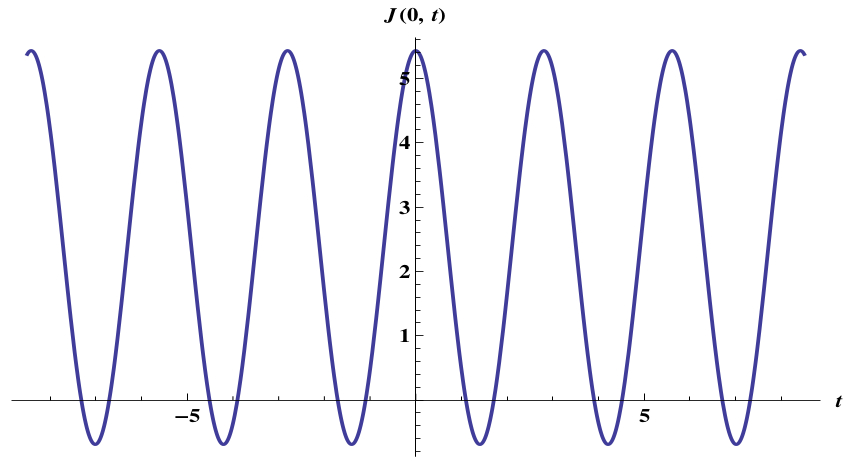
\includegraphics[scale=0.25]{images/plane_wave}
%	\caption{as}
%	\label{fig:plane_wave}
%\end{figure}
Although this example has no physical interpretation, because of the non-normalizability of plane waves, we can note that backflow is essentially an interference effect between some wave-packets with high positive momentum and others with low positive momentum. This aspect is not trivial and we will we re-use it for proving an important theorem regarding the intensity of backflow through a single point at a some instant of time. In particular, we will construct a normalized wave-packet in momentum space as a sum of a function $\tilde{\chi}(p)\in L^2(\mR_+)$ and its translation $\tilde{\chi}(p-n)$, with $n\in\mathbb{N}$. This coincides with taking the interference of two wave-packets with different positive momenta.

\subsection{Superposition of Gaussian Wave-packets}
\label{sec:gaussian}
Another example can be made by replacing the two plane waves with Gaussian functions tightly picked in momentum. This represents a more physically realistic state. We consider the sum of two initial Gaussian wave-packets with equal
spatial width $\sigma$, evolved for a time $t$. The corresponding normalized wave function is
\begin{multline}
	\psi(x,t)=\sum_{n=1,2}C_n\frac{1}{\sqrt{4\sigma^2+2it}}\exp\left(ip_n(x-p_nt)-\frac{(x-p_nt)^2}{4\sigma^2+2it}\right),\\ \ C_n\in\mR,\ p_1,p_2>0.
\end{multline}
This function was proposed by Yearsley in [\citealp{years}]. As in the previous example, this wave-function is given by the superposition of two waves with different momentum. Note that as $\sigma\to0$, we obtain once more a superposition of plane waves. To prove that for such a function backflow occurs, we set the parameters $p_1,p_2,C_1,C_2$ and $\sigma$ to be
\begin{equation}
\label{eq:parameters}
p_1 = 0.3, \ p_2 = 1.4,\ C_1 = 1.8,\ C_2 = 1,\ \sigma= 10.
\end{equation}
We plot the probability $P(t)$ of the particle being localized at a point $x < 0$ as a function of time, see Figure \ref{fig:back_2}. Observe that $P(t)$ is non monotonically decreasing, but in several disjoint time intervals it increases, proving the presence of backflow.

\begin{figure}[h]	
\centering
\begin{minipage}{0.45\textwidth}
		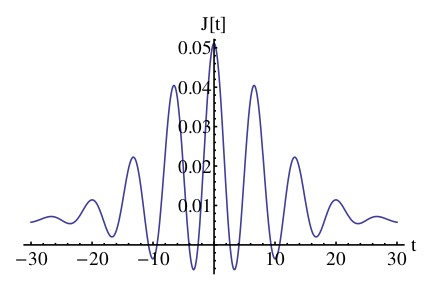
\includegraphics[scale=0.43]{images/gaussian_1}
		\caption{Plot of the current for a superposition of
			two gaussians, with the parameters given in Eq. [\ref{eq:parameters}].}
		\label{fig:back}
\end{minipage}
\hfil
\begin{minipage}{0.45\textwidth}
		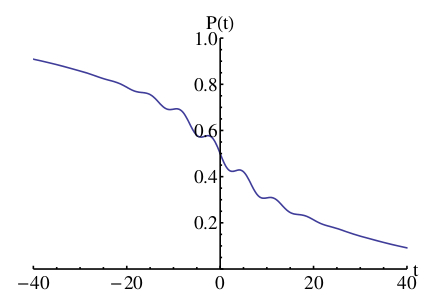
\includegraphics[scale=0.43]{images/gaussian_2}
		\caption{Plot of the probability for
			remaining in $x < 0$ for a superposition of two gaussians,
			with the parameters given in Eq. [\ref{eq:parameters}]. }
		\label{fig:back_2}
\end{minipage}
\end{figure}
One might wonder how to quantify the amount of backflow that this state displays. To answer this query, we need to evaluate
\begin{equation}
	P(t_1)-P(t_2)=\int_{t_1}^{t_2}\nspace\!j_\psi(0,t)\, \dd t,
	\label{eq:prob_flux}
\end{equation} 
where $P$ is the probability of finding the particle within the domain $x<0$ while $[t_1 , t_2 ]$ is the interval maximizing the amount of backflow for this wave-function. A direct evaluation shows that,
\begin{equation}
	F:=\mathrm{inf}\{P(t_1)-P(t_2)\ |\ t_2>t_1 \}\approx -0.0061
\end{equation}
We will see in the following discussion that this flux is approximately the 16\% of the maximum amount of backflow theoretically allowed. 
\subsection{Normalizable Wave}

The following example shows that backflow can also occur for normalizable wave-functions. Let us consider $\phi\in L^2(\mR)$ whose representation in the momentum space (which is nothing more than its Fourier transform $\hat{\phi}$) is given by the following equation:
\begin{equation}	
	\hat{\phi}(p)=\begin{cases}
	\frac{18}{\sqrt{35K}}p(e^{-p/K}-\frac{1}{6}e^{-p/2K}) & p>0\\
	0 & p\le 0
	\end{cases}
	\label{ex2:def}
\end{equation}
where $K$ is a positive constant. This represents a possible initial state for a physical particle. Now we can write the expression for the function $\phi$ defined in the position space:
\begin{equation}
\begin{aligned}
	&\phi(x)=18\sqrt{\frac{K}{70\pi}}\left[\frac{1}{(1-iKx)^2}-\frac{2}{3(1-2iKx)^2}\right].
\end{aligned}\label{ex2:position}
\end{equation}
At this point we can evaluate $\phi(0)$, $\phi'(0)$ and the density probability current $j_\phi(0)$ as:
\begin{equation}
\begin{aligned}
&\phi(0)=6\sqrt{\frac{K}{70\pi}} & \phi'(0)=-12i\sqrt{\frac{K}{70\pi}}\\
& j_\phi(0)=-\frac{36K^2}{35\pi }<0,
\end{aligned}
\end{equation}
which proves the presence of backflow. Evaluating the time evolution of this wave-function, the current is negative during the interval $[0,t_1]$ where $t_1 \approx 0.021/K^2$. The corresponding flux, from (\ref{eq:prob_flux}), is
\begin{equation}
	F\approx-0.0043
\end{equation}

\section{Backflow in Free Theory}
In this section we want to study the length and the strength of this effect in the case of free particles. In particular, The question we ask ourselves is:
\begin{verse}
	\centering
\emph{What is the maximum amount of probability which could flow back through a point $x_0$ during an interval of time $T$ for a right-moving free-particle?}
\end{verse}
We will show that this problem is equivalent to finding the smallest eigenvalue of a suitable integral operator, out of which one establish a bound for quantum backflow.\\
In the following discussion we will interpret the flux of probability defined in Eq. (\ref{eq:prob_flux}) in a time interval $[0,T]$ through a certain point, say the origin $x=0$, as a scalar product of the form $(\hat{\psi}|\theta B_T \theta \hat{\psi})$, where $\hat{\psi}$ is the Fourier transform of the wave-function (i.e. right-mover), $\theta$ is the Heaviside function and $B_T$ is the \textit{backflow operator} that will be proved to be bounded and self-adjoint. After that, we will link the upper bound for this operator to the evaluation of the maximum eigenvalue of an integral operator $K$ (defined by Bracken and Melloy in [\citealp{bracken}]). Furthermore, we will show that this maximum eigenvalue corresponds to the maximum amount of backflow allowed for any right-mover. In this part of our thesis will report the results obtained by Penz \textit{et al.} in [\citealp{penz}].\\
\subsection{Temporal Boundedness of Backflow}
Let us start by considering how the free Schr\"{o}dinger evolution operator acts in momentum space. We have shown in Section \ref{sec:quantum_mechanincs} that for a wave-function represented in the Fourier-transformed space $\hat{\psi}$, the evolution operator $U_t$ could be transformed into a phase multiplicative operator:
 \begin{equation}
 	\hat{\psi}_t(p)=\widehat{U_t\psi}=(\widehat{U}_t\hat{\psi})(p)=e^{-ip^2t/2}\hat{\psi}(p)\, ,
 	\label{eq:unitary_evolution}
 \end{equation}
 where we introduced the operator $\widehat{U}_t:=\mathcal{F}U_t\mathcal{F}^{-1}$.
 
 \begin{oss}
 	Notice that, if $\psi\in E_+L^2(\mR)$, then, by definition of $\widehat{U}_t$, $U_t\psi\in E_+ L^2(\mR)$ for all $t\in\mathbb{R}$. Stated differently, the evolution preserves the subspace $E_+L^2(\mR)$ of right-mover wave-functions. Furthermore, we observe that $U_t^*=U_{-t}$ and $\widehat{U}_t^*=\widehat{U}_{-t}$. 
 	\label{oss:widehat(U)}
 \end{oss}
  The representation of such wave-functions in the "position" space are given by the anti-Fourier transform:
\begin{equation}
\psi_t(x)=\frac{1}{\sqrt{2\pi}}\int_{-\infty}^{+\infty}\nspace\! e^{ipx}\hat{\psi}_t(p)\, \dd p.
\end{equation}
Let a particle be described in momentum space by a wave-function $\hat{\psi}(p)$ at time $0$. If $\|\hat{\psi}\|=\|\psi\|=1$, the probability that a position measurement at time $t$ yields a position $x > 0$ reads
\begin{equation}
	L(\psi_t):=\int_{0}^{+\infty}\nspace\!|\psi_t(x)|^2\, \dd x=(\hat{\psi}|\widehat{U}^*_t\mathcal{F}\theta\mathcal{F}^{-1} \widehat{U}_t\hat{\psi}).
\end{equation}
Now we restrict to consider right-moving wave-functions $\psi$ such that $E_+\psi=\psi$ or equivalently $\theta\hat{\psi}=\hat{\psi}$ and $\|\psi\|=1$. Note that for such functions the evolution $\psi_t$ is also a right-mover, $\psi_t=E_+\psi_t$.\\
 As shown in the previous examples, there exist right-moving wave-functions in which backflow occurs and the probability $L(\psi_t)$ does decrease in a time interval. So, it is convenient to define the maximum backflow for a fixed right-mover $\psi$ as
\begin{equation}
	\lambda(\psi)=\sup\{L(\psi_s)-L(\psi_t)\ |\ s,t\in\mR,\ t>s \}
	\label{eq:lambda_psi}
\end{equation}
Since we are interested in the maximum amount of probability backflow, we define the \textbf{backflow constant} $\lambda$ as
\begin{equation}
	\lambda:=\sup\{\lambda(\psi)\ |\ \psi=E_+\psi,\ \|\psi\|=1 \}.
	\label{eq:backflow_const}
\end{equation}
Introducing the orthogonal projector $\tilde{\theta}_t:=\widehat{U}^*_t\mathcal{F}\theta\mathcal{F}^{-1} \widehat{U}_t$ we obtain for any normalized wave-function $\psi\in L^2(\mR)$
\begin{equation}
	L(\psi_s)-L(\psi_t)=(\hat{\psi}|(\tilde{\theta}_s-\tilde{\theta}_t)\hat{\psi}).
\end{equation}
Since
\begin{equation}
	\tilde{\theta}_s-\tilde{\theta}_t=\widehat{U}^*_{\frac{t+s}{2}}(\tilde{\theta}_{\frac{s-t}{2}}-\tilde{\theta}_{\frac{t-s}{2}})\widehat{U}_{\frac{t+s}{2}},
\end{equation}
we can write
\begin{equation}
	\lambda=\sup\{  (   \hat{\psi}  |  \widehat{U}^*_{\tau}(\tilde{\theta}_{-T}-\tilde{\theta}_{T})\widehat{U}_{\tau}\hat{\psi}) \ |\ \psi=E_+\psi,\ \|\psi\|=1,\ \tau\in\mR,\ T>0\},
\end{equation}
\begin{definition}
	Given a fixed time $T>0$, we call \textbf{backflow operator} $B_T:L^2(\mR)\to L^2(\mR)$
	\begin{equation}
		B_T:=\tilde{\theta}_{-T}-\tilde{\theta}_T.
		\label{eq:backflow_operator}
	\end{equation}
\end{definition}
$B_T$ enjoys the following properties
\begin{prop}
	\label{prop:backflow_operator}
	The operator $\theta B_T\theta$ with $B_T$ defined in (\ref{eq:backflow_operator}) is bounded and self-adjoint.
\end{prop}
\begin{proof}
	The boundedness of $\theta B_T\theta$ follows from the boundedness of $\theta$ and $\widehat{U}_T$ forall $T\in\mR$. One can prove self-adjointness by considering the scalar product $(\psi|\theta B_T\theta \phi)$ for some $\psi,\phi\in L^2(\mR)$ and see that it is equal to $(\theta B_T\theta\psi|\phi)$ using self-adjointness of $\theta$ and the definition of adjoint for $\widehat{U}_T$.
\end{proof}

\begin{oss}
	Note that the operator $\theta$ here needs to cut the negative momenta of a wave-function transforming it into a right-mover.
\end{oss}

Focusing on the analysis of the backflow constant $\lambda$, since $\widehat{U}_\tau$ preserves the set of right-movers $E_+(L^2)$, see Observation \ref{oss:widehat(U)}, it holds
\begin{equation}
	\lambda=\sup\{(\phi|\theta B_T\theta \phi)\ |\ \phi\in L^2(\mR),\ \|\phi\|=1,\ T>0 \},
\end{equation} 
or equivalently 
\begin{equation}
	\lambda=\sup\bigcup_{T>0}\sigma(\theta B_T\theta).
	\label{eq:lambda_sum}
\end{equation}

\begin{oss}
	(\ref{eq:lambda_sum}) could be simplified by neglecting the set sum over $T>0$. In fact we see that $\theta B_T\theta$ is the operator which gives the flux of probability through the origin $x=0$ for a time interval $[0,T]$. Using scaling arguments, one shows that backflow is independent from the time $T$, in the sense that, for every right-mover with some amount of backflow during the interval $[0,T]$, there exists another right-mover with the same backflow, but for a time interval $[0,T']$ arbitrarily larger.
\end{oss}

\begin{prop}
	For any fixed time $T>0$, $\lambda=\sup \sigma(\theta B_T\theta)$.
	\label{prop:time_independence}
\end{prop}
\begin{proof}
	Consider the family of unitary operators $V_\mu:L^2(\mR)\to L^2(\mR) $ with $\mu>0$ defined as $(V_\mu\phi)(p):=\sqrt{\mu}\phi(\mu p)$. For any $\phi\in L^2(\mR)$
	\begin{equation}
		(\theta V_\mu \phi)(p)=\sqrt{\mu}\theta(p)\phi(\mu p)=\sqrt{\mu}\theta(\mu p)\phi(\mu p)=(V_\mu\theta\phi)(p),
	\end{equation}
	and
	\begin{equation}
		\mathcal{F}\theta\mathcal{F}^{-1}V_\mu\phi=\mathcal{F}\theta V_{1/\mu}\mathcal{F}^{-1}\phi=\mathcal{F} V_{1/\mu}\theta\mathcal{F}^{-1}\phi=V_\mu	\mathcal{F}\theta\mathcal{F}^{-1}\phi.
	\end{equation}
	Then $V_\mu$ commutes with both the operator $\theta$ and $	\mathcal{F}\theta\mathcal{F}^{-1}$. Note that $V_\mu^*=V_{1/\mu}$. A direct calculation shows that
	\begin{equation}
		V_\mu \widehat{U}_t V_\mu^*= \widehat{U}_{\mu^2t}
	\end{equation}
	It follows that
	\begin{equation}
		V_\mu\theta B_T \theta V_\mu^*=\theta B_{\mu^2T}\theta.
	\end{equation}
	Since the spectrum of an operator is invariant under a unitary transformation we have for any $T_1,T_2>0$
	\begin{equation}
	\sigma(\theta B_{T_1}\theta)=\sigma(V_{\mu'}\theta B_{T_1} \theta V_{\mu'}^*)=\sigma(\theta B_{T_2}\theta)\ \text{ where } \ \mu'=\sqrt{T_2 / T_1}.
	\end{equation}
    Hence we can write $\lambda=\sup\sigma(\theta B_{T_1}\theta)$ for any fixed $T>0.$
\end{proof}

Summing up all results we obtained for the backflow operator $B_T$ and for the backflow constant $\lambda$, it holds.

\begin{theorem}[\textbf{Temporal Boundedness of Backflow}]
	\label{th:temp_bound}
	Let $\lambda=\sup \sigma(\theta B\theta)$, where $B=B_{T=1}$ is the backflow operator. For any right-mover $\psi\in L^2(\mR)$ such that $\psi=E_+\psi$ and for any $T>0$ it holds 
	\begin{equation}
		\int_{0}^{T}\nspace\!j_\psi(0,t)\, \dd t\ge -\lambda>-\infty.
	\end{equation}
\end{theorem}
\begin{proof}
	Since $\lambda$ is the maximum amount of backflow, we must to prove that it is finite. Since the operator $\theta B\theta$ is bounded and self-adjoint (in view of Proposition \ref{prop:backflow_operator})
	\begin{equation}
		\sigma( \theta B\theta) \subseteq [-\|B\|,\|B\|].
	\end{equation}
	Hence the sought thesis descends.
\end{proof}

Once we proved temporal boundedness of backflow for free particles, we are interested about evaluating numerically the backflow constant $\lambda$ introducing the integral operator first founded by Bracken and Melloy in [\citealp{bracken}]. These authors heuristically introduce $\lambda$ via time integrals of currents at point $x = 0$ over arbitrary finite intervals, motivating their definition of $\lambda$ as the supremum of the spectrum of such integral operator.

\begin{prop}
	\label{prop:bracken_int}
	Let $K:L^2(\mR_+)\to L^2(\mR_+)$ be the integral operator:
	\begin{equation}
	\label{eq:bracken_int}
		(Kf)(u)=-\frac{1}{\pi}\int_{0}^{\infty}\frac{\sin(u^2-v^2)}{u-v}f(v)\, \dd v \ \ \forall f\in L^2(\mR_+).
	\end{equation}
	Then $\theta B\theta f  = Kf$ for all $f\in L^2(\mR_+)$. 
\end{prop}
\begin{proof}
	Since $\theta B \theta$ is bounded we only need to prove that $\theta B\theta  = K$ holds on a dense subspace of $L^2(\mR_+)$. Hence, we choose $\mathcal{S}(\mR_+):=\theta\mathcal{S}(\mR)$, i.e. the set of Schwartz functions projected with the Heaviside function.\\% the space of all smooth functions, rapidly decreasing and with support contained in $\mR_+$.\\
	First of all, we relate the orthogonal projection $\mathcal{F} \theta \mathcal{F}^{-1}$ to the Hilbert transform
	\begin{equation}
		\begin{aligned}
		& H:L^2(\mR)\to L^2(\mR), & (Hf)(p)=\frac{1}{\pi}PV\nspace\int_{-\infty}^{\infty}\frac{f(q)}{p-q}\, \dd q.
		\end{aligned}
	\end{equation} 
	Here $PV$ indicates the principal value. For $f\in\mathcal{S}(\mR)$ we obtain by means of Lebesgue's dominated convergence theorem and by means of Sochozki's formula ,see [\citealp[Example 3.3.1]{blanch}],
	\begin{equation}
		\begin{aligned}
		(\mathcal{F} \theta \mathcal{F}^{-1}f)(p) &= \frac{1}{2\pi}\int_{0}^{\infty}\nspace\!e^{-ipx}\left(\int_{-\infty}^{\infty}\nspace\!e^{ixq}f(q)\, \dd q\right)\, \dd x\\
		&= \frac{1}{2\pi}\lim_{\varepsilon\to 0^+}\int_{-\infty}^{\infty}\nspace\!f(q)\left(\int_{0}^{\infty}\nspace\!e^{i(q-p)x-\varepsilon x}\, \dd x\right)\, \dd q\\
		&= -\frac{1}{2\pi i}\lim_{\varepsilon\to 0^+}\int_{-\infty}^{\infty}\frac{f(q)}{q-p+i\varepsilon}\dd q\\
		&= -\frac{1}{2\pi i}\left\{ PV\nspace\int_{-\infty}^{\infty}\frac{f(q)}{q-p}\, \dd q-i\pi f(p)\right\}\\
		&= \frac{1}{2i}(Hf)(p)+\frac{f(p)}{2}.
		\end{aligned}
	\end{equation}
	Hence, we have 
	\begin{equation}
	\label{eq:backflow_hilbert}
		\mathcal{F} \theta \mathcal{F}^{-1}=\frac{1}{2}(-iH+\mathbb{I}).
	\end{equation}
	Now consider the backflow operator defined as $B=U\mathcal{F} \theta \mathcal{F}^{-1}U^*-U^*\mathcal{F} \theta \mathcal{F}^{-1}U$, where $U:=\widehat{U}_{T=1}$ is the unitary evolution operator in momentum space defined in (\ref{eq:unitary_evolution}). Substituting (\ref{eq:backflow_hilbert}) into the last equation, we obtain
	\begin{equation}
		B=\frac{1}{2i}(UHU^*-U^*HU).
	\end{equation}
	From this we have for $p>0$ and $\phi\in \mathcal{S}(\mR_+)$
	\begin{equation}
	\begin{aligned}
	(\theta B\theta \phi)(p)&=\frac{e^{-ip^2}}{2i}(HU^*\phi)(p)-\frac{e^{ip^2}}{2i}(HU\phi)(p)\\
	&= \frac{1}{2\pi i}\int_{0}^{\infty}\frac{e^{-i(p^2-q^2)}-e^{i(p^2-q^2)}}{p-q}\phi(q)\, \dd q\\
	&= -\frac{1}{\pi}\int_{0}^{\infty}\frac{\sin(p^2-q^2)}{p-q}\phi(q)\dd q=(K\phi)(p).
	\end{aligned}	
	\end{equation}
	Thus the restriction of $\theta B\theta \phi$ to $L^2(\mR_+)$ coincides with $K$.
\end{proof}
\begin{oss}
	With the last proposition we proved that searching the maximum amount of backflow for any right-movers is equivalent to finding the supremum of the spectrum of a suitable integral operator. Furthermore, we have that for a generic right-mover $\psi=E_+\psi$ with $\|\psi\|=1$
	\begin{equation}
	L(\psi_{t=0})-L(\psi_{t=1})=(\hat{\psi}|K\hat{\psi}),
	\end{equation}
	where $L(\psi_t)$ is the probability of finding the particle in $x>0$ at the time $t$, and $K$ the operator defined in Proposition \ref{prop:backflow_operator}.
\end{oss}

\subsection{Maximum Backflow Approximation}
	As we proved in Theorem \ref{th:temp_bound}, there exists a lower bound for backflow. To wit, for every time interval $[0,T)$ the maximum amount of probability which could flow back for a generic right-mover is always less than $|\lambda|$. We have no information concerning $\lambda$ and its eigenfunction $\phi_\lambda$. To solve this quandary, we need to study the integral operator $K$. Unfortunately, no analytical value for $\sup \sigma(K)$ is known, and numerical methods have been used to estimate $\lambda$. \\
	More precisely, we approximate $\mR_+\times\mR_+$ by $[0,N\tau]\times[0,N\tau]$ divided into a grid of $N^2$ squares of area $\tau^2$. In each square we approximate the kernel of the integral operator as a constant. At the same time we approximate the eigenfunction $\phi_{\lambda}$ as a vector $\varphi_\lambda^i$ in $\mC^n$ by considering the function constant in each interval $[i\tau,(i+1)\tau]$ with $i=1,...,n$.\footnote{see [\citealp[Sect. 5]{bracken}]} In this way we are converting our eigenvalue-problem to a linear equation:
	\begin{equation}
		-\frac{1}{\pi}\int_{0}^{\infty}\frac{\sin(u^2-v^2)}{u-v}\varphi(v)\, \dd v=\lambda\varphi(u) \stackrel{\approx}{\longmapsto} K_k^i\varphi_\lambda^k=\lambda\varphi_\lambda^i,
		\label{eq:eigenvalue_approx}
	\end{equation}
	where $K_k^i$ is the hermitian matrix obtained by approximating our integral kernel. The second equation admits a solution. In order to find a good estimate for $\lambda$ we need to take $N\to\infty$ and $\tau\to0$. Here we report some results obtained by Braken and Melloy in their work considering $\tau=0.05$. The estimates obtained are:
	\begin{center}
		\centering
		\footnotesize
		\begin{tabular}{|c|cccc|}
			\toprule
			$N$ & 100 & 200 & 275 & 500\\
			\midrule
			$\lambda$ & 0.0256 & 0.0297 & 0.0309 & 0.0323\\
			\bottomrule
		\end{tabular}
		%\caption{Estimation of maximum backflow via grid approximation}
	\end{center}
	which are apparently converging to $\lambda_{0.05}\approx0.034$. Taking smaller values of $\tau$ and letting $N\to\infty$ we obtain the estimates $\lambda_{0.04}\approx0.035$, $\lambda_{0.025}\approx0.036$ and $\lambda_{0.01}\approx0.038$.\\% Recent research had been calculated numerically with more accuracy over the years the eigenvalue $\lambda$ and estimates it to be $\approx-0.0384517$.
	
	A possible method to compute the maximum eigenvalue $\lambda$ is given by Penz in [\citealp{penz}]. It is based on an algorithm called \textit{power iteration} and it works as follows.\\
	Let $A\in\mC^{N\times N}$ be a symmetric matrix and let $a$ be the eigenvalue of $A$ with the largest absolute value. Then, consider a vector $v_0\in\mC^N$ such that $v_0\neq0$ and there is a non-zero component within the eigenspace of $A$ corresponding to $a$. Then the sequence $\{v_n\}_{n\in\mathbb{N}_0}$ recursively defined by
	\begin{equation}
		v_{n+1}=\frac{Av_n}{\|v_n\|}
	\end{equation}
	converges to a normalized eigenvector of $a$. In addition, it holds\footnote{see [\citealp[Sect. 7.3.1]{matrix}]}
	\begin{equation}
		a=\lim_{n\to\infty}v_{n+1}^\dagger\frac{v_n}{\|v_n\|}.
	\end{equation}
	
	Since $\sigma(\theta B \theta)=\sigma(K)\subset[-1,\lambda]$, the power method can be applied to the non negative, discretized operator $\theta B\theta+\mathbb{I}$. Its largest eigenvalue then approximates $\lambda +1$ while the sequence $v_n$ tends to the maximizing eigenvector.\\
	Penz started his calculations by covering a square $[0,q_0]^2$ with $N_0$ grid points and subsequently he repeated the computations for up to $N=N_0h$ grid points and a larger square $ [0,q]^2$ with $q=q_0\sqrt{h}$ for $h=1,2,$ etc.. With this method, we can at the same time make the square growing and the absolute step size getting smaller. This leads to a sequence of eigenvalues $\lambda_h$ as a function of the factor of accuracy $h$ which are used to extrapolate to $h\to\infty$ and getting an approximation $\lambda_\infty$ of the backflow constant. The results obtained by Penz are plotted in figure \ref{fig:backflow_approx_1} and \ref{fig:backflow_approx_2}.\\
	\begin{figure}[h]	
		\centering
		\begin{minipage}{0.45\textwidth}
			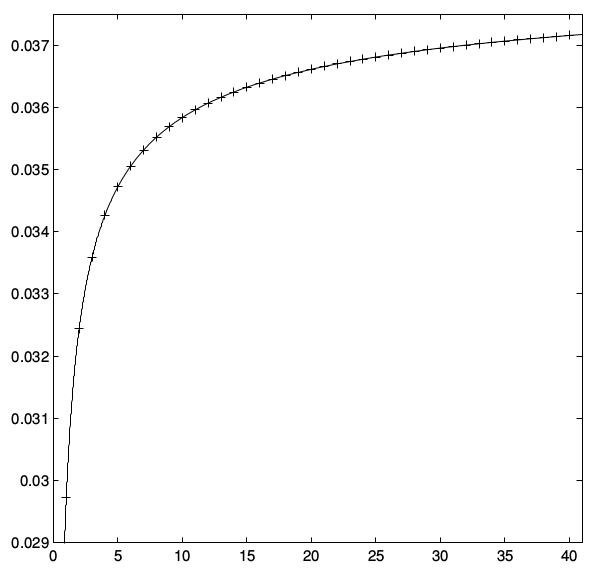
\includegraphics[scale=0.31]{images/backflow_approx_1}
			\caption{$\lambda$ plotted against $h$ and fit $\lambda_\infty+b/\sqrt h$.}
			\label{fig:backflow_approx_1}
		\end{minipage}
		\hfil
		\begin{minipage}{0.45\textwidth}
			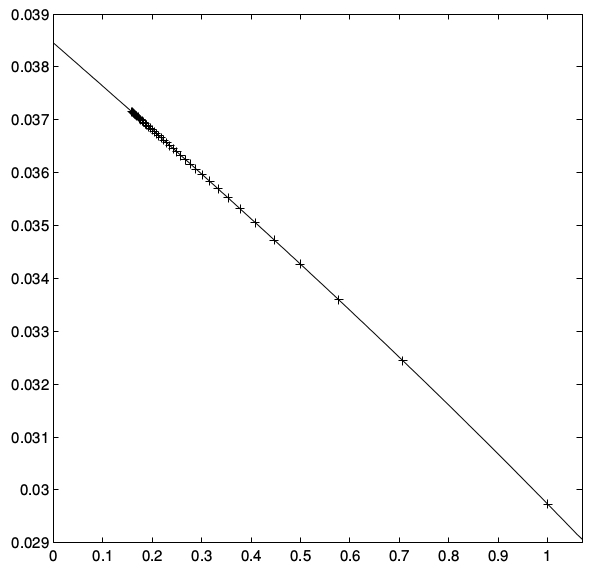
\includegraphics[scale=0.31]{images/backflow_approx_2}
			\caption{$\lambda$ plotted against $1/\sqrt h$ and polynomial fit of third order.}
			\label{fig:backflow_approx_2}
		\end{minipage}
	\end{figure}
	
	The approximation for the backflow constant can be read off from the intersection of the $y$-axis with the graph in (\ref{fig:backflow_approx_2}). This yields
	\begin{equation}
		\lambda\approx\lambda_\infty\approx 0.0384517.
	\end{equation}
	This is the final result computed by Penz \textit{et al.} in [\citealp{penz}]. Another analysis has been done by Eveson, Fewster and Verch in [\citealp{verch}] giving an approximation for the backflow constant by $\lambda\approx 0.038452$.\\
	
	
	
	

 % Include the second content chapter
\chapter{Interacting Quantum Backflow}
The final chapter will be dedicated to the analysis of backflow in scattering theory. First of all, we shall discuss the spatial extension of backflow showing that a negative probability current might occur on arbitrary large region of space but its average value is bounded from below. After that, we extend the analysis of backflow to interacting systems, given by fairly general Hamiltonians of the form $H = P^2/2 + V(X)$, see Section \ref{sec:quantum_mechanincs}.\\
There are two main issues concerning interacting situations:
\begin{itemize}
	\item[(a)] In the free case, a right-mover will preserve positive momentum for every time. In the interacting case, this is no longer true. Consider a potential which reflects the particle. The reflected wave-function entails the presence of a \textit{classic backflow}\footnote{Since the reflected wave goes in the opposite direction of the incident wave, this contributes negatively to the probability flux.} which sums up with its quantum counterpart. This is a conceptual problem since we want to study the strength of the only quantum backflow.
	\item[(b)] In free theory, backflow is based on right-moving wave-function. Since in the interacting case this property is no longer preserved, we need to reformulate the problem of backflow.
\end{itemize}
%After that we will focus on proving th existence of probability backflow also in the presence of a potential $V(X)$ with some little restricting properties. For this purpose we need to reformulate the concept of right-moving in scattering situation introducing the "interaction picture" of quantum mechanics mentioned in Chapter \ref{chapter1}.\\
%The importance of such analysis lies on the fact that the presence of scattering potentials are far more likely than totally free case. If we want to study a possible experimental set-up for observing backflow, we could never be able to cancel all possible potential. Furthermore, since backflow is a really weak phenomenon, also little potentials could interfere strongly with measurements. Hence, a study of backflow in scattering situations is necessary.\\ 
In the following discussion, we will focus mainly on [\citealp{gand}] and report their main results.
\section{Spatially Averaged Backflow}
In the last section we investigated some properties of backflow for free right-moving particles. We find out that, no matter for how long a wave function is let to evolve, the amount of probability flowing across a reference point, as per (\ref{eq:prob_flux}), is always larger than a dimensionless constant $-\lambda\approx-0.038$. This is a bound on the (averaged) temporal extent of backflow. Up to this, we studied backflow and the associated density probability current only at a reference point $x=0$. We focus now the corresponding (averaged) spatial extension. In particular we want to understand how negative values of $j_\phi$ could be distributed by considering spatial integrals of the kinematical current. In particular we will find out a lower bound similar to the one discovered in the previous section. More precisely, we will show that for all normalized right-movers $\phi$ and all positive averaging functions $f\ge0$, exists $c_f\in\mR$ such that:
\begin{equation}
\int_{\mR}\!\! f(x)j_\phi(x)\, \dd x\ge c_f>-\infty
\label{eq:spatial_bound}
\end{equation}
Here the function $f$ plays the role of an extended detector, generalizing the step function that we used in (\ref{eq:prob_flux}).\\
To start with, we report a result obtained in [\citealp{gand}] concerning the possible values of the density current $j_\phi$ for a normalized right-moving wave function $\phi$ evaluated in $x=0$.
\begin{prop}[\textbf{Unboundedness of $j_\phi$}]
	\label{prop:unboundedness}
	Let $x\in\mR$. Then there exist sequences $\phi_n^\pm\in E_+(L^2(\mR))$ of right-moving wave functions such that 
	\begin{equation}
	\lim_{n\to\infty}j_{\phi_n^\pm}(x)=\pm\infty,
	\end{equation}
	and the norms $\|\phi_n^\pm\|_{L^2}^2$ and $\|\hat{\phi}_n^\pm\|_{L^1}$ are independent of $n$.
\end{prop}
\begin{proof}
	Consider a right-moving wave function $\phi^+\in E_+L^2(\mR)$ and define $\hat{\phi}_n^+(p):=\hat{\phi}^+(p-n)$, with $n\in\mathbb{N}$. It holds $\|\hat{\phi}_n^+\|_{L^1}= \|\hat{\phi}^+\|_{L^1}$ and $\|\phi_n^+\|_{L^2}^2=\|\phi^+\|_{L^2}^2$ for all $n\in\mathbb{N}$. Furthermore, using the relation $\phi_n^+=e^{inx}\phi^+$, and (\ref{eq:density_current})
	\begin{equation}
	j_{\phi_n^+}(x)=j_{\phi^+}(x)+n|\phi^+(x)|^2,
	\end{equation}
	Hence, if we choose $\phi^+$ such that $\phi^+(x)\neq0$, $\lim_{n\to\infty}j_{\phi_n^+}(x)=+\infty$. To focus in the other option, we choose a wave function $\chi$ such that $\hat{\chi}$ has compact support on $x\in(0,\infty)$ and $\chi\neq0$. Such function is by construction a right-mover. Now we consider the linear combinations $\hat{\phi}_n^-(p):=\alpha_n\hat{\chi}(p)+\beta_n\hat{\chi}(p-n)$, where $n\in\mathbb{N}$, and $\{\alpha_n\},\{\beta_n\}\in\mC$ are sequences such that $|\alpha_n|=\alpha$ and $|\beta_n|=\beta$ are constant for all $n\in\mathbb{N}$. By construction, each $\phi_n^-$ is a right-mover and, for large $n$, $\|\phi_n^-\|_{L^2}^2=(|\alpha|^2+|\beta|^2)\|\chi\|_{L^2}^2$ while $\|\hat{\phi}_n^-\|_{L^1}=(|\alpha|+|\beta|)\|\chi\|_{L^1}$. At this point, it only remains to choose $\alpha$ and $\beta$ in order to have $\lim_{n\to\infty}j_{\phi_n^-}(x)=-\infty$. With this purpose, we can evaluate $j_{\phi_n^-}(x)$ obtaining:
	\begin{equation}
	j_{\phi_n^-}(x)=\begin{pmatrix}\alpha^*\\ \beta^* \end{pmatrix}^t[j_\chi(x)\mathbb{I}+nA_n]\begin{pmatrix}\alpha \\ \beta	\end{pmatrix},
	\end{equation}
	where
	\begin{equation}
	A_n:=\begin{bmatrix}
	0 & e^{inx}\left(\frac{j_\chi(x)}{n}+\frac{|\chi(x)|^2}{2}\right)\\
	e^{-inx}\left(\frac{j_\chi(x)}{n}+\frac{|\chi(x)|^2}{2}\right) & |\chi(x)|^2
	\end{bmatrix}\, .
	\end{equation}
	Here $A_n$ is a $2\times2$ Hermitian matrix, whose trace is $|\chi(x)|^2$, and $\lim_{n\to\infty}\det(A_n)=-|\chi(x)|^4/4<0$. The eigenvalues $\lambda_\pm(n)$ of $A_n$ converge to $\lambda_\pm(n)\to (1\pm\sqrt{2})|\chi|^2/2$ as $n\to\infty$. Finally, choosing $\alpha_n$ and $\beta_n$ as the coordinates of the eigenvector with the negative eigenvalue $(1-\sqrt{2})|\chi|^2/2$ (i.e. take $\alpha_n=1/(1-\sqrt{2})$ and $\beta_n=\exp(-inx)$) we can  check that $\lim_{n\to\infty}j_{\phi_n^-}(x)=-\infty$ because of the explicit factor $n$ in front of $A_n$.
\end{proof}
\begin{oss}
	Before turning back to the main goal of this section, we note that the density current function $j_\psi$ could be thought as a quadratic form defined as
	\begin{equation}
	(\psi|J(x)\psi):=j_\psi(x),
	\end{equation}
	Here $J(x)$ could be defined as an "improper" operator (see [\citealp{years2}]) via
	\begin{equation}
	J(x_0)=\frac{1}{2}[P\delta(X-x_0)+\delta(X-x_0)P],
	\end{equation}
	where $\delta(X)$ is the \textit{Dirac delta distribution}.
\end{oss}
We can rewrite the spatially averaged density current by means of $f\in\mathcal{S}(\mR)$ as:
\begin{equation}
(\phi|J(f)\phi):=\int_{\mR} f(x)j_\phi(x)\, \dd x,
\end{equation}
where $J(f)$ can be readily checked to be an (unbounded) operator, Hermitian for real $f$, and decomposable in terms of the position and momentum operator ($X$,$P$) as follows.
\begin{definition}
	Let $f\in\mathcal{S}(\mR)$. We define the \textbf{density current operator} $J(f)$ as:
	\begin{equation}
	J(f)=\frac{1}{2}[Pf(X)+f(X)P]\,.
	\label{eq:density_operator}
	\end{equation}
\end{definition}
\begin{rem}
	Note that the operator $E_+J(f)E_+$ represents the averaged current evaluated in right-moving states. The fact that backflow exists is reflected in  $E_+J(f)E_+$ being non positive. To formulate this concept more rigorously we can introduce the \textbf{bottom of the spectrum} of a Hermitian operator $A$ defined as
	\begin{equation}
	\inf(A):=\inf_{\|\phi\|=1}(\phi|A\phi)\in[-\infty,+\infty).
	\end{equation}
	The maximal amount of backflow, spatially averaged by $f$, is defined as
	\begin{equation}
	\beta_0(f):=\inf(E_+J(f)E_+)\, .
	\end{equation}
	Observe the similarities with the definition of the constant backflow $\lambda$ as the infimum of a bounded and self-adjoint operator $B$.
\end{rem}
 Next we summarize three fundamental properties of the operator $J(f)$. The first one is the \textit{existence} of backflow showing that $\beta_0(f)<0$ for each positive test function $f$, and more strongly \textit{for each} function $f\neq0$. The second property is the unboundedness of $E_+J(f)E_+$ from above that will be proved similarly to Proposition \ref{prop:unboundedness}. The final point regards the existence of a lower bound for our averaged current operator. In fact it will be proved that $\beta_0(f)>-\infty$, in contrast with the last Proposition where $j_\phi(x)$ has been shown to be unbounded.
 
\begin{theorem}[\textbf{Existence and boundedness of spatially averaged Backflow}]
	\label{th:ex_averaged_backflow}
	In the context of quantum backflow, the following proposition are true:
	\begin{itemize}
		\item[(a)] For any $f\in\mathcal{S}(\mR)$ with $f\neq0$, the smeared probability flow in any right-moving wave-function, $E_+J(f)E_+$, is non positive, that is $\beta_0(f)<0$.
		\item[(b)]Let $f>0$. Then $E_+J(f)E_+$ is not upper bounded.
		\item[(c)]Let $f>0$. Then $E_+J(f)E_+$, is lower bounded, i.e. $\beta_0(f)>-\infty$. Furthermore, for any test functions $f=g^2$, for $g\in\mathcal{S}(\mR)$, it holds\footnote{see [\citealp{verch}]}
		\begin{equation}
		\beta_0(g^2)\ge-\frac{1}{8\pi}\int_{\mR}\!\! |g'(x)|^2\, \dd x>-\infty.
		\label{eq:ineq_gsquare}
		\end{equation}
	\end{itemize}
\end{theorem}
\begin{proof}
	(a) First of all, we consider the operator $E_+J(f)E_+$ and $\phi\in L^2(\mR)$. It holds
	\begin{equation}
	\begin{aligned}
	& \mathcal{F}E_+J(f)E_+\phi=\mathcal{F}E_+J(f)\mathcal{F}^{-1}\mathcal{F}E_+\phi=\theta(q)\mathcal{F}J(f)\mathcal{F}^{-1}\theta(p)\hat{\phi}(p)= \\
	& = \frac{1}{2}\mathcal{F}f(x)\mathcal{F}^{-1}(p+q)\theta(q)\theta(p)\hat{\phi}(p)=\int_{-\infty}^{\infty}\nspace\!\dd p\, \frac{p+q}{2\sqrt{2\pi}}\hat{f}(q-p)\theta(p)\theta(q)\hat{\phi}(p).
	\end{aligned}
	\end{equation}
	Hence we have identified the integral kernel
	\begin{equation}
	K_f(q,p)=\frac{p+q}{2\sqrt{2\pi}}\hat{f}(q-p)\theta(p)\theta(q),
	\end{equation}
	Taking the restriction of $K_f$ to $L^2(\mR_+,\dd p)$, we can neglect the Heaviside functions.\\
	We shall prove non-positivity of $E_+J(f)E_+$ by contradiction. Hence, suppose $E_+J(f)E_+$ were positive. Then,
	\begin{equation}
	\int_{0}^{+\infty}\nspace\nspace\dd q\,\int_{0}^{+\infty}\nspace\nspace \dd p\, \varphi^*(q)K_f(q,p)\varphi(p)>0\ \forall\varphi\in L^2(\mR_+,\dd p)\, .
	\end{equation}
	Consider a sequence $\{g_n\}\in L^2_0(\mR)$ of functions converging to the Dirac delta distribution $\delta_0$, and $\alpha,\beta\in\mC$. It holds 
	\begin{multline}
	\int_{0}^{+\infty}\nspace \nspace \dd q'\,\int_{0}^{+\infty}\nspace\nspace \dd p'\, [\alpha^*g_n^*(q'-q)+\beta^*g_n^*(q'-p)]K_f(q',p')\times\\ \times[\alpha g_n(q'-q)+\beta g_n(q'-p)]>0,
	\end{multline}
	for all $n\in\mathbb{N}$, $\alpha,\beta\in\mC$, and $p,q>0$. So, taking the limit $n\to\infty$,
	\begin{equation}
	\begin{pmatrix}
	\alpha \\\beta
	\end{pmatrix}^\dagger
	\begin{bmatrix}
	K_f(q,q) & K_f(q,p)\\
	K_f(q,p) & K_f(p,p)
	\end{bmatrix}
	\begin{pmatrix}
	\alpha\\ \beta
	\end{pmatrix}>0\  \forall \alpha,\beta\in\mC,\ \forall p,q>0.
	\label{eq:matrix_average_backflow}
	\end{equation}
	In this paragraph we have proved $E_+J(f)E_+$ is positive if so is the Hermitian $2\times2$ matrix (\ref{eq:matrix_average_backflow}) for each choice of $p,q>0$. This amounts to the matrix must having only non-negative eigenvalues, which in turn is implemented by a non-negative determinant and trace. The former reads
	\begin{equation}
	0\le K_f(q,q)K_f(p,p)-|K_f(q,p)|^2=\frac{pq}{2\pi}|\hat{f}(0)|^2-\frac{(p+q)^2}{8\pi}|\hat{f}(q-p)|^2\, \
	\end{equation}
	i.e. 
	\begin{equation}
	|\hat{f}(q-p)|\le\frac{2\sqrt{pq}}{p+q}|\hat{f}(0)|.
	\end{equation}
	Now we can show that, taking $q\to0$ at fixed $p>0$, $|\hat{f}(-p)|=0$ for all $p>0$. Yet, since $f$ is real, $\hat{f}(-p)=\hat{f}^*(p)$, so that $\hat{f}(p)=0$ for each $p\neq0$. As the test function $f$ is continuous, this implies that $f$ vanishes altogether. So we conclude that for any real $f\neq0$ the operator $E_+J(f)E_+$ is not positive.\\
	(b) The proof of this point is pretty similar to the one of Proposition \ref{prop:unboundedness}. In fact, consider a normalized right-moving function $\phi=E_+\phi \in L^2(\mR)$, and define a sequence of shifted-momentum wave functions $\hat{\phi}_n(p)=\hat{\phi}(p-n)$ with $n\in\mathbb{N}$. It holds that $\|\phi_n\|_{L^2}=1$ and $E_+\phi_n=\phi_n$. Furthermore, the expectation value of $E_+J(f)E_+$ is
	\begin{equation}
	(\phi_n|E_+J(f)E_+\phi_n)=(\phi|E_+J(f)E_+\phi)+n\int_{-\infty}^{+\infty}\nspace\!\! f(x)|\phi(x)|^2\, \dd x.
	\end{equation} 
	For $f>0$, it is clear that there exists $\phi$ such that the last integral is positive and in this case we have $\lim_{n\to\infty}(\phi_n|E_+J(f)E_+\phi_n)=+\infty$, showing that the operator $E_+J(f)E_+$ has no finite upper bound.\\
	(c) In order to prove the final statement of this theorem, we consider a general normalized right-moving function $\phi=E_+\phi\in L^2(\mR)$ and $g\in\mathcal{S}(\mR)$. The averaged spaced density current reads
	\begin{equation}
	\begin{aligned}
	(\phi|E_+J(g^2)E_+\phi)& = Re(\phi|g^2(X)P\phi)\\
	& = Re[(\phi|g(X)Pg(X)\phi)+(\phi|g(X)[g(X),P]\phi)]\\
	& = Re[(\phi|g(X)Pg(X)\phi)+i(\phi|g(X)g'(X)\phi)]\\
	& = Re(\phi|g(X)Pg(X)\phi)=(g(X)\phi|Pg(X)\phi)\\
	& = \int_{-\infty}^{+\infty}\nspace\!p|\mathcal{F}[g(X)\phi](p)|^2\, \dd p.
	\end{aligned}
	\end{equation}
	Here $[g(X),P]$ is equal to $ig'(X)$. Considering the integral only on $(-\infty,0)$, we obtain:
	\begin{equation}
	(\phi|E_+J(g^2)E_+\phi)\ge\int_{-\infty}^{0}\nspace\! p|\mathcal{F}[g(X)\phi](p)|^2\, \dd p=-\int_{0}^{\infty}\nspace\!p|\mathcal{F}[g(X)\phi](-p)|^2\, \dd p.
	\label{eq:gsquare}
	\end{equation}
	By the Convolution Theorem \ref{th:conv_theorem} we can rewrite $\mathcal{F}[g(X)\phi]$ as
	\begin{equation}
	\mathcal{F}[g(X)\phi](p)=\frac{1}{\sqrt{2\pi}}\int_{0}^{\infty}\nspace\! \dd p'\, \hat{\phi}(p')\hat{g}(p-p'),
	\end{equation}
	where the restriction to $p'>0$ is a consequence $E_+\phi=\phi$. Now, applying the Cauchy-Schwarz theorem, we obtain:
	
	\begin{equation}
	\begin{aligned}
	|\mathcal{F}[g(X)\phi](-p)|^2&=\left|\frac{1}{\sqrt{2\pi}}\int_{0}^{\infty}\nspace\nspace \dd p'\, \hat{\phi}(p')\hat{g}(-p-p')\right|^2\\ &\le\frac{\|\phi\|^2}{2\pi}\int_{0}^{\infty}\nspace\! \dd p'\, |\hat{g}(-p-p')|^2=
	\frac{1}{2\pi}\int_{0}^{\infty}\nspace\! \dd p'\, |\hat{g}(p+p')|^2,
	\end{aligned}
	\end{equation}
	where we have also used $|\hat{g}(-p)|^2=|\hat{g}(p)|^2$ (being $g$ real valued) and $\|\phi\|=1$. Substituting into (\ref{eq:gsquare}),
	\begin{equation}
	\begin{aligned}
	(\phi|E_+J(g^2)E_+\phi)& \ge -\frac{1}{2\pi}\int_{0}^{\infty}\nspace\nspace \dd p\,\int_{0}^{\infty}\nspace\nspace \dd p'\, p|\hat{g}(p+p')|^2\\
	& = -\frac{1}{2\pi}\int_{0}^{\infty}\nspace\nspace \dd u\, |\hat{g}(u)|^2\int_{0}^{u}\nspace \dd p\, p\\
	& = -\frac{1}{4\pi}\int_{0}^{\infty}\nspace\nspace \dd u\, u^2|\hat{g}(u)|^2\\
	& = -\frac{1}{8\pi}\int_{-\infty}^{\infty}\nspace\nspace \dd u\, u^2|\hat{g}(u)|^2\\
	& = -\frac{1}{8\pi}\int_{-\infty}^{\infty}\nspace\nspace \dd x\, |g'(x)|^2 \ \forall \phi\in L^2(\mR),
	\end{aligned}
	\end{equation}
	where we have changed the variables $(p,p')$ to $(u,p)$ with $u=p+p'$. We enjoyed that  $|\hat{g}(u)|^2$ is even as well as and Parseval's theorem . This last equation complete the proof of the inequality (\ref{eq:ineq_gsquare}). This also proves the boundedness of $E_+J(f)E_+$ for all Schwarz functions $f>0$ since there always exists $g\in\mathcal{S}(\mR)$ such that $g^2=f$. 
\end{proof}

Until now, we considered right-moving functions at a fixed time and no assumption on any potentials has been made so far. In the following section we start the analysis of backflow in scattering theory by introducing the concept of \textit{interacting state} and \textit{asymptotic solutions} of Schr\"{o}dinger equation.

\section{Backflow and Scattering}

Let us consider a physical system described by an Hamiltonian $H=\frac{1}{2}P^2+V(X)$, where $V(X)$ is a general time-independent potential described as a function of the position $X$. We wonder whether backflow could occur and if there exists a lower bound for the averaged spatial density current. The first conceptual problem that we encounter is that in non-zero potential situation, the space of right-movers $E_+(L^2(\mR))$ is no longer invariant under time evolution. Hence, it is more difficult to define when a particle "travels to the right"\footnote{see [\citealp[Sect. III]{gand}]}. To overcome this, we can substitute the concept of right-moving solutions with the "asymptotic momentum" distributions in the sense of scattering theory. Heuristically, we consider solutions such that for $t\to-\infty$ the associated wave-function is a right-mover in the usual sense. This space has the property to be invariant under time evolution and describes particles scattering "from the left" into the potential wall. The link between an asymptotic, free state $\psi$ and the interacting counterpart is ruled by the \textit{M\o{}ller operator}:
\begin{equation}
\Omega_V:=\lim_{t\to-\infty}e^{iHt}e^{-iH_0t},
\end{equation}
where $H_0$ is the free Hamiltonian $P^2/2$. As mentioned in Chapter \ref{chapter1} the last equation has to be read in this way\footnote{see [\citealp[Chapt. 0, Sect. 4]{scattering}]}: Consider a particle which scatters against a potential wall $V$ at the time $t=0$. Its dynamics is described by Schr\"{o}dinger equation
\begin{equation}
	i\partial_t\psi(t)=H\psi(t),\ \ \psi(0)=\psi_0\, ,
\end{equation}
Until the particle is sufficiently distant from the potential wall, it behaves like a free particle. Stated differently, we state that $\psi(t)$ has "free" asymptotics as $t\to-\infty$ if there exists $u_0\in L^2(\mR)$ such that
\begin{equation}
	\lim_{t\to-\infty}\|\psi(t)-u(t)\|=0,\ \ u(t):=\exp(-iH_0t)u_0\, .
	\label{eq:free_asymptotics}
\end{equation}
Relation (\ref{eq:free_asymptotics}) leads to a connection between the corresponding initial data $\psi_0$ and $u_0$,
\begin{equation}
	\psi_0=\lim_{t\to-\infty}e^{iHt}e^{-iH_0t}u_0=\Omega_Vu_0.
\end{equation}
\begin{oss}
	Observe that, although $\Omega_V$ is not unitary in the presence of bound states, we still have $\|\Omega_V\| = 1$.\\
\end{oss} 

We focus on the averaged probability current $J(f)$ in an asymptotically right-moving state.

\begin{definition}
	Let $J(f)$ be the density current operator defined in (\ref{eq:density_operator}), and let $E_+$  be the orthogonal projector on the space of right-movers. Let $\Omega_V$  be the M\o{}ller operator. We call $E_+\Omega_V^*J(f)\Omega_VE_+.$  the \textbf{asymptotic current operator}
\end{definition}
\begin{rem}
	The goal of this section is to investigate the spectral properties of this operator, and how to estimate the \textit{backflow constant}:
	\begin{equation}
	\beta_V(f):=\inf(E_+\Omega_V^*J(f)\Omega_VE_+).
	\end{equation}
\end{rem}
For scattering theory to be well defined, we need to impose our potentials $V(x)$ to be sufficiently rapidly decreasing as $x\to\pm\infty$.
\begin{definition}
	We define $L^{1+}(\mR)$ the set of all real functions $V$ such that the norm
	\begin{equation}
		\|V\|_{1+}:=\int_{-\infty}^{\infty}\nspace\! (1+|x|)|V(x)|\, \dd x < \infty
	\end{equation}
	exists finite.
\end{definition}
\begin{oss}
Let  $V\in L^{1+}$, the time-independent Schr\"{o}dinger equation for scattering states reads:
	\begin{equation}
	[-\partial_x^2+2V(x)-k^2]\psi(x)=0\ k\in\mR.
	\label{eq:stationary_eq}
	\end{equation}
	In the stationary picture of scattering theory, we seek solutions $\varphi_k$, $k>0$, of (\ref{eq:stationary_eq}) with the following asymptotics:
	\begin{equation}
	\label{eq:asymptotics}
	\varphi_k(x)=\begin{cases}
	T_V(k)e^{ikx}+o(1) & \text{for }  x\to+\infty\\
	e^{ikx}+R_V(k)e^{-ikx}+o(1) & \text{for } x\to-\infty
	\end{cases}
	\end{equation}
	where $R_V(k)$ and $T_V(k)$ denote the reflection and transmission coefficients of the potential $V$, respectively, and are uniquely determined by $V$. In other words we choose all those solutions behaving like plane waves which scatter against a potential wall, resulting into a transmitted plane wave $e^{ikx}T_V(k)$ and into a reflected one $R_V(k)e^{-ikx}$ (See Fig. (\ref{fig:asymptotics})).
\end{oss}
\begin{figure}[h]
	\centering
	\begin{tikzpicture}
	\usetikzlibrary{fadings}
	
	\draw [->, very thick] (4.3,0.5) -- (5.3,0.5) ;
	\draw [->, very thick, blue] (6.2,0) -- (5.5,0) ;
	\draw [->, very thick, blue] (10.8,0.2) -- (11.6,0.2) ;
	\node at (5,1) {$e^{ikx}$};
	\node [blue] at (6.8,0.7) {$R_Ve^{-ikx}$};
	\node [blue] at (10.5,0.9) {$T_Ve^{ikx}$};
	\node [red] at (9.2,1) {$V(x)$};
	\draw [black] plot [smooth] coordinates {(3.5,0)  (3.625,1) (3.75,-1) (4,1) (4.2,-1) (4.4,1) (4.6,-1) (4.75,0)};
	
	\draw [blue] plot [smooth] coordinates {(6,0)  (6.125,0.4) (6.25,-0.4) (6.5,0.4) (6.7,-0.4) (6.9,0.4) (7,0)};
	\shade[top color=red!30,bottom color=white, draw=red] plot [smooth] coordinates {(7,-0.75) (7.8,-0.4) (8.5,0.9) (8.75,0.9) (9.4,-0.4) (10.2,-0.75)};
	
	\draw [blue] plot [smooth] coordinates {(10,0)  (10.125,0.6) (10.25,-0.6) (10.5,0.6) (10.7,-0.6) (10.9,0.6) (11,0)};
	\end{tikzpicture}
	\label{fig:asymptotics}
	\caption{Sketch of a scattering process of a plane wave with momentum $k$ into a potential $V(x)$ resulting into reflected and transmitted waves as Eq. (\ref{eq:asymptotics})}
\end{figure}
 At this point, we shall recall a few results of scattering theory. A deeper and more exhaustive analysis of the mathematical aspects of scattering theory could be found in [\citealp{scattering}].
\begin{lem}
	\label{lem:ex_of_sol}
	Let $V\in L^{1+}(\mR)$. Then the M\o{}ller operator $\Omega_V$ exists. Furthermore, the solution $x\mapsto\varphi_k(x)$ ($k>0$) of (\ref{eq:stationary_eq}) with the asymptotic conditions (\ref{eq:asymptotics}) exists and it is unique. In addition, for any $\hat{\psi}\in C_0^\infty(\mR)$,
	\begin{equation}
		(\Omega_VE_+\psi)(x)=\frac{1}{\sqrt{2\pi}}\int_{0}^{\infty}\nspace\!\varphi_k(x)\hat{\psi}(k)\, \dd k.
		\label{eq:asymptotic_sol}
	\end{equation}
\end{lem}

We will stick to report the references where finding an exhaustive proof of this lemma. Existence and uniqueness of solution $\varphi_k$ are a consequence of [\citealp[Chap. 5, Lemma 1.1]{scattering}]. Existence of $\Omega_V$, under milder assumptions on $V$, can be found in [\citealp[Chap. 5, Theorem 1.12]{scattering}].\\
\begin{oss}
	Let us dwell further on the meaning of Eq. (\ref{eq:asymptotic_sol}). We are considering a smooth wave-function $\psi$ with momentum representation $\hat{\psi}\in C^\infty_0(\mR)$, though we are interested only in "right-moving" solutions. Then, we will not consider the function $\hat{\psi}(k)$ for $k<0$. Considering only the "right-moving" components of $\psi$ we can think of it as the sum of plane wave-functions $e^{ikx}\hat{\psi}(k)$ (parametrized in $k>0$) which scatter into the potential $V$ giving the solutions $\varphi_k$. The integral of all this scattered components will give the solution $\Omega_VE_+\psi$.%them as independent plane wave-functions $e^{ikx}\hat{\psi}(k)$ (parametrized in $k>0$) which scatter into the potential $V$ giving the solutions $\varphi_k$. In the end, we just sum up all the interacting components in order to find out the solution $\Omega_VE_+\psi$.
\end{oss}
\begin{rem}
	From here on, we will consider only wave-functions $\psi$ such that $\hat{\psi}\in C^\infty_0(\mR)$ as in Lemma \ref{lem:ex_of_sol} in order to have a well defined asymptotic current operator $E_+\Omega_V^*J(f)\Omega_VE_+$.
\end{rem}

\begin{oss}
	Using (\ref{eq:asymptotic_sol}), we are able to estimate the expectation values of the asymptotic current operator as follows
	\begin{equation}
	(\psi|E_+\Omega^*_VJ(f)\Omega_VE_+\psi)=\int_{-\infty}^{\infty}\nspace\!\dd x\,f(x)\int_{0}^{\infty}\nspace\!\dd p\,\int_{0}^{\infty}\nspace\!\dd q\, \hat{\psi}^*(p)K_V(p,q,x)\hat{\psi}(q),
	\label{eq:density_product}
	\end{equation}
	where $K_V$ is
	\begin{equation}
	K_V(p,q,x)=\frac{i}{4\pi}[\partial_x\varphi_p^*(x)\varphi_q(x)-\varphi_p^*(x)\partial_x\varphi_q(x)].
	\label{eq:K_V}
	\end{equation}
\end{oss}

Following [\citealp{gand}], the next step in our analysis is to establish bounds on the solution $\varphi_k$ and $K_V$ relating them to their spatial asymptotics. As in the previous lemma, we will not give any proof, but only pointing to relevant references.
\begin{lem}
	\label{lem:bounds}
	Let $V\in L^{1+}(\mR)$ and let $\varphi_k$, with $k>0$, be the solution of (\ref{eq:stationary_eq}) with the asymptotics (\ref{eq:asymptotics}). Let $K_V$ be as in (\ref{eq:K_V}). Then, there exist constants $c_V,c_V',c_V'',c_V'''>0$ such that for all $x\in\mR$ and $p,q,k>0$
	\begin{align}
	%\begin{equation}
	|\varphi_k(x)|&\le c_V(1+|x|), \label{eq:bounds_1}\\
	%\end{equation} 
	%\begin{equation}
	 |\varphi_k(x)e^{ikx}|&\le c_V'\frac{1+|x|}{1+k}, \label{eq:bounds_2}\\
	%\end{equation} 
	%\begin{equation}
	 |\partial_x\varphi_k(x)-ik\varphi_k(x)|&\le c_V''\frac{1}{1+k}, \label{eq:bounds_3}\\
	%\end{equation} 
	%\begin{multline}
	 \left|K_V(p,q,x)-\frac{p+q}{4\pi}\varphi_p^*(x)\varphi_q(x)\right|&\le c_V'''(1+|x|). \label{eq:bounds_4}
	\end{align}
\end{lem}
The first two bounds in (\ref{eq:bounds_1}) and (\ref{eq:bounds_2}) can be deduced from [\citealp[Sec. 2, Lemma 1]{deift}], paying attention to the fact that the function $m(x,k)$ there corresponds to our $\varphi_k(x)e^{-ikx}/T_V(k)$, while $T_V(k)$ is such that $|T_V(k)|\le1$ and $T_V(k)=1+O(1/k)$ for large $k$ [\citealp[Sec. 2, Theorem 1]{deift}]. The last two bounds in (\ref{eq:bounds_3}) and (\ref{eq:bounds_4}), are consequence of (\ref{eq:bounds_1}) and (\ref{eq:bounds_2}). The constants $c_V,c_V',c_V'',$ and $c_V'''$ can be deduced from [\citealp{deift}] as functions of $V$, although they are not optimal and we will not use them during the following discussion.\\
With this information in mind, we have arrived to the first main result for backflow in scattering theory. We will prove the unboundedness of the asymptotic current operator $E_+\Omega_V^*J(f)\Omega_VE_+$ and the existence of backflow as well as the presence of negative parts of the spectrum, generalizing the results of the free situation, see Th. \ref{th:ex_averaged_backflow}.
\begin{theorem}[\textbf{Existence of backflow in scattering situations}]
	\label{th:ex_scat_back}
	Let $V\in L^{1+}(\mR)$. Then,
	\begin{itemize}
		\item[(a)] for every $f\in\mathcal{S}(\mR)$ with $f>0$, there is no finite upper bound on the asymptotic current operator $E_+\Omega_V^*J(f)\Omega_VE_+$,
		\item[(b)] for every $x\in\mR$, there is a sequence of normalized right-movers $\psi_n=E_+\psi_n$ such that $\lim_{n\to\infty}(\psi_n|\Omega_V^*J(x)\Omega_V\psi_n)=-\infty$.
	\end{itemize}
\end{theorem}
\begin{oss}
	Before proving Theorem \ref{th:ex_scat_back}, let us note that point (b) means that the backflow constant $\beta_V(f)$ could be negative for some positive $f$. Thus, averaged backflow exists in all scattering situations. The difference with the free case is that $\beta_0(f)$ ought to be negative for all positive Schwarz functions $f$, see Th. \ref{th:ex_scat_back} In scattering scenarios, we are not able to give an analogous statement for $\beta_V(f)$.
\end{oss}

\begin{proof}[Proof of Theorem \ref{th:ex_scat_back}]
	(a). To prove unboundedness of $E_+\Omega_V^*J(f)\Omega_VE_+$, we recall what done in Theorem \ref{th:ex_averaged_backflow} (b). Hence, we consider a right-mover $\psi=E_+\psi$ such that $\hat{\psi}\in C^\infty_0(\mR_+)$ and shift it to higher momenta defining the sequence $\hat{\psi}_n(p):=\hat{\psi}(p-n)$. In view of the unboundedness of $(\psi_n|E_+J(f)E_+\psi_n)$ from above [as in Theorem \ref{th:ex_averaged_backflow}(b)], we only need to show that the sequence $(\psi_n|(\Omega_V^*J(f)\Omega_V-J(f))\psi_n)$ is bounded as $n\to\infty$. In fact, from (\ref{eq:density_product}) it holds
	\begin{multline}
		(\psi_n|(\Omega_V^*J(f)\Omega_V-J(f))\psi_n)=\int_{-\infty}^{\infty}\nspace\! \dd x\, f(x)\int_{\mR_+^2}\dd p\,\dd q\,\times\\
		 \times\bigg\{\hat{\psi}^*_n(p)\hat{\psi}_n(q)\left[K_V(p,q,x)-\frac{p+q}{4\pi}\varphi_p^*(x)\varphi_q(x)\right]+\\
		 +\hat{\psi}^*(p)\hat{\psi}(q)\frac{p+q+2n}{4\pi}\left[\varphi_{p+n}^*(x)\varphi_{q+n}(x)-e^{i(q-p)x}\right]\bigg\},
	\end{multline}
	where $\varphi$ are the solutions taken from Lemma \ref{lem:ex_of_sol}. Since the norms $\|\hat{\psi}_n\|_{L^1}$ are independent from $n$, the first integrand is bounded in view of (\ref{eq:bounds_4}). (\ref{eq:bounds_1}) and (\ref{eq:bounds_2}) yield the same for the second integrand. This proves point (a).\\
	(b) Non-positivity of the asymptotic current operator $E_+\Omega_V^*J(f)\Omega_VE_+$ could be proved similarly. Here we take a sequence of right-movers $\psi_n^-$  as in Proposition \ref{prop:unboundedness}. Then, it suffices to show that $(\psi_n|(\Omega_V^*J(f)\Omega_V-J(x))\psi_n)$ is bounded in the same way as in point (a), using a suitable choice of $\chi$, such that $\hat{\chi}\in C^\infty_0(\mR_+)$) as in Proposition \ref{prop:unboundedness}.
\end{proof}

Now, we are ready for the main result of this chapter: the boundedness of the backflow constant $\beta_V(f)$ for every fixed non-negative $f\in\mathcal{S}(\mR)$, with potential $V\in L^{1+}(\mR)$. For this purpose, we need to take the asymptotic current operator $E_+\Omega_V^*J(f)\Omega_VE_+$ and split it into several terms (see in Observation (\ref{oss:split})).
\begin{oss}
	\label{oss:T_V}
	Consider the projector into the "left-movers" space $E_-$ from Definition \ref{def:projector_E+} and let the operator $T_V$ act by multiplication with the transmission coefficient $T_v(k)$ from (\ref{eq:asymptotics}) in momentum space. Hence, it holds true that
	\begin{itemize}
		\item[(i)]$T_V$ commutes with $E_\pm$ and $E_-T_VE_+=E_-E_+T_V=0$. The first statement descends from $E_\pm$ anf $T_V$ being defined as multiplicative operators in momentum space and the second from the identity $E_\pm E_\mp=0$.
		\item[(ii)]$E_-\Omega_VE_+=E_-(\Omega_V-T_V)E_+$ as consequence of point (i).
	\end{itemize}
\end{oss}

\begin{oss}[\textbf{Bounds of current operator}]
	\label{oss:split}
	Via the identities $E_-+E_+=\mathbb{I}$ and $(i+P)^{-1}(i+P)=\mathbb{I}$, it holds
	\begin{equation}
	\label{eq:split}
	\begin{aligned}
	E_+\Omega_V^*J(f)\Omega_VE_+&=E_+\Omega_V^*(E_-+E_+) J(f)(E_-+E_+)\Omega_VE_+\\
	& =E_+\Omega_V^*E_+ J(f)E_+\Omega_VE_+\\
	&+ E_+\Omega_V^*E_+J(f)(i+P)^{-1}E_-(i+P)(\Omega_V-T_V)E_+\\
	&+ E_+(\Omega_V^*-T_V^*)(-i+P)E_-(-i+P)^{-1}J(f)\Omega_VE_+.
	\end{aligned}
	\end{equation}
	Here we used the results from Observation \ref{oss:T_V}, the commutativity between $(i+P)$ and $E_\pm$ and $(i+P)^*=(-i+P)$. Note that the first term on the right side of (\ref{eq:split}) is bounded by the constant $\beta_0(f)$, as proved in Theorem \ref{th:ex_averaged_backflow}, and $\|E_+\|=\|\Omega_V\|=1$.\\
	We must evaluate the other terms on the right hand side of (\ref{eq:split}) in order to prove the existence of maximum backflow. In particular we want to show that
	\begin{equation}
	\begin{aligned}
	\inf(E_+\Omega_V^*J(f)\Omega_VE_+)&\ge \beta_0(f) -2\|J(f)(i+P)^{-1}\|\|(i+P)(\Omega_V-T_V)E_+\|\\ &\ge \beta_0(f)-2\|J(f)(i+P)^{-1}\|[2+\|P(\Omega_V-T_V)E_+\|],
	\end{aligned}
	\label{eq:split2}
	\end{equation}
	where the norms $\|J(f)(i+P)^{-1}\|$ and $\|P(\Omega_V-T_V)E_+\|$ ought to be finite.
\end{oss}

In order to estimate $\|J(f)(i+P)^{-1}\|$, it is useful to introduce the concept of Green's distribution. The Green distribution, or fundamental solution, of a linear differential operator $L$ is the distribution $G$ such that $LG=\delta$, where $\delta$ is the Dirac's delta distribution\footnote{see [\citealp[Chapt. 5, Sect. 3-4]{fried2}]}. In our case, we are interested in finding the Green's function of the time-independent Schr\"{o}dinger equation (\ref{eq:stationary_eq}).
\begin{prop}
	Consider the function $G_k(x)$ defined as 
	\begin{equation}
		G_k(x):=\frac{\sin(kx)}{k}\theta(x).
	\end{equation}
	Then, $G_k$ is the solution of equation $-G_k''(x)=k^2G_k(x)-\delta(x)$ in the sense of distributions, i.e. $G_k$ is the fundamental solution of the time-independent Schr\"{o}dinger equation (\ref{eq:stationary_eq}).
	\label{prop:green}
\end{prop}
The solution $\varphi_k$ of (\ref{eq:stationary_eq}) could be uniquely determined using $G_k$ via the following integral equation (Lippman-Schwinger equation) 
\begin{equation}
	\varphi_k(x)=T_V(k)e^{ikx}+\int_{-\infty}^{\infty}\nspace\! 2V(y)G_k(y-x)\varphi_k(y)\, \dd y,
	\label{eq:lippman}
\end{equation}
where (\ref{eq:lippman}) is the convolution between $G_k$ and $\varphi_k\cdot V$. With this information at hand,
\begin{prop}
	\label{prop:bound5}
	Let $V\in L^{1+}(\mR)$. Then
	\begin{equation}
		\|P(\Omega_V-T_V)E_+\|\le 2c_V\|V\|_{1+}\, ,
	\end{equation}
	with the constant $c_V$ being the one in Lemma \ref{lem:bounds}.
\end{prop}
\begin{proof}
	Consider $\xi,\psi$ such that $\hat{\xi},\hat{\psi}\in C_0^\infty(\mR)$ and $\psi=E_+\psi$. Lemma \ref{lem:ex_of_sol} yields
	\begin{equation}
	\begin{aligned}
	(\xi|P(\Omega_V-T_V)\psi)&=(P\xi|(\Omega_V-T_V)\psi)\\ &=\frac{i}{\sqrt{2\pi}}\int_{-\infty}^{\infty}\nspace\!\dd x\, {\xi'}^*(x)\int_{0}^{\infty}\nspace\! \dd k\, [\varphi_k(x)-T_V(k)e^{ikx}]\hat{\psi}(k).
	\end{aligned}
	\end{equation}
	The expression above may be rewritten in view of (\ref{eq:lippman}), using Fubini's theorem and integration by parts. Thus, we obtain
	\begin{equation}
	\label{eq:bound_5}
	\begin{aligned}
	(\xi|P(\Omega_V-T_V)\psi)&=\frac{i}{\sqrt{2\pi}}\int_{-\infty}^{\infty}\nspace \dd x\, {\xi'}^*(x)\int_{0}^{\infty}\nspace\!\dd k\,\int_{-\infty}^{\infty}\nspace\! \dd y\, 2V(y)G_k(y-x)\varphi_k(y).\\
	& = \frac{2i}{\sqrt{2\pi}}\int_{\mR^2}\nspace\!\dd x\,\dd y\int_{0}^{\infty}\nspace\!\dd k\, \xi(x)^*V(y)\cos[k(y-x)]\theta(y-x)\varphi_k(y)\hat{\psi}(k)
	\end{aligned}
	\end{equation}
	Consider the multiplicative operator $M_y$, with $y\in\mR$, defined as
	\begin{equation}
		(M_y\psi)(k):=\mathcal{F}^{-1}[\varphi_k(y)\hat{\psi}(k)]
	\end{equation}
	and the integral operator $I_y$
	\begin{equation}
		(I_y\hat{\psi})(x):=\theta(y-x)\int_{0}^{\infty}\nspace\!\cos[k(y-x)]\hat{\psi}(k)\, \dd k.
	\end{equation}
	As noted in [\citealp[Prop. 2]{gand}], %the last equation consists of a projection onto only the positive and even momentum part of $\psi$, a multiple of the Fourier transform, a multiplication by the Heaviside function, and a change of variables $x\mapsto y-x$. Thus,
	 $\|I_y\|\le\sqrt{2\pi}$ for all $y\in\mR$. Using Lemma \ref{lem:bounds} and (\ref{eq:bounds_1}), we establish the following bound for $M_y$:
	\begin{equation}
		\|M_y\psi\|\le (c_V(1+|y|))\|\psi\|\Rightarrow \|M_y\|\le c_V(1+|y|)\ \forall y\in\mR.
	\end{equation}
	Replacing the previous bounds in (\ref{eq:bound_5}), yields
	\begin{equation}
	\begin{aligned}
	|(\xi|P(\Omega_V-T_V)\psi)|&\le \frac{2\|\xi\|\|\psi\|}{\sqrt{2\pi}}\int_{-\infty}^{\infty}\nspace\!|V(y)|\|I_y\|\|M_y\|\,\dd y\\
	&\le 2c_V\|\xi\|\|\psi\|\int_{-\infty}^{\infty}\nspace\!|V(y)|(1+|y|)\,\dd y\\ &\le 2c_V\|V_y\|_{1+}\|\xi\|\|\psi\|.
	\end{aligned}
	\end{equation}
	Since $\xi$ and $\psi$ are taken respectively from a dense subspace of $L^2(\mR)$ and $E_+L^2(\mR)$, this concludes the proof.
\end{proof}

Summing up all results obtained in Observation \ref{oss:split}, (\ref{eq:split}), and Proposition \ref{prop:bound5}, it holds the following\footnote{see [\citealp[Th. 3]{gand}]}
\begin{theorem}[\textbf{Boundedness of backflow in scattering situations}]
	\label{th_backflow_scat}
	For any potential $V\in L^{1+}(\mR)$ and for any non-negative $f\in\mathcal{S}(\mR)$, there exists a lower bound on the spatially averaged backflow:
	\begin{equation}
		\beta_V(f)\ge\beta_0(f)-[2\|f\|_{\infty}+\|f'\|_{\infty}](2+2c_V\|V\|_{1+})>-\infty,
		\label{eq:backflow_scat}
	\end{equation}
	where $\|f\|_{\infty}:=\sup_{x\in\mR}|f(x)|$, $\beta_0(f)$ is the backflow constant in Th. \ref{th:ex_averaged_backflow}, and $c_V$ is the constant from Lemma \ref{lem:bounds}.
\end{theorem}
\begin{proof}
	To prove this bound we reconsider (\ref{eq:split2})
	\begin{equation}
		\inf(E_+\Omega_V^*J(f)\Omega_VE_+)\ge \beta_0(f)-2\|J(f)(i+P)^{-1}\|[2+\|P(\Omega_V-T_V)E_+\|].
		\label{eq:split3}
	\end{equation}
	Following Observation \ref{oss:split}, we must prove the existence of a bound for $\|P(\Omega_V-T_V)E_+\|$ and $\|J(f)(i+P)^{-1}\|$. The first one is given by Proposition \ref{prop:bound5}. To prove that for $\|J(f)(i+P)^{-1}\|$, we note from the definition of $J(f)$ in (\ref{eq:density_operator}) that
	\begin{equation}
		J(f)=\frac{1}{2}[Pf(X)+f(X)P]=\frac{1}{2}\bigg[[P,f(X)]+2f(X)P\bigg]=f(X)P-\frac{i}{2}f'(X).
	\end{equation}
	Hence we have $\|J(f)(i+P)^{-1}\|\le \|f\|_{\infty}+\frac{1}{2}\|f'\|_{\infty}$. Replacing everything in (\ref{eq:split3}), the thesis follows.
\end{proof} 

The last theorem concludes our investigation on the existence of backflow in an interacting scenario. We have shown that the asymptotic current operator $E_+\Omega_V^*J(f)\Omega_VE_+$ is bounded from below. Thus, in any scattering scenario backflow can occur, but its value spatially averaged under a non-negative test-function $f$ is always bigger than the constant $\beta_V(f)$. Note that \eqref{eq:backflow_scat} says very little about the actual value of this bound and a numerical analysis is needed for different types of potentials $V$. Some examples are given in [\citealp[Sect. IV]{gand}]. % Include the third content chapter
\chapterstyle{thesis2} % Change the style of the Chapter header to that defined in structure.tex
\chapter*{Conclusions}
\label{conclusions}
\addcontentsline{toc}{chapter}{Conclusions}
\thispagestyle{plain}
In this thesis we described the local and global well-posedness of wave-like equations propagating on a curved globally hyperbolic Lorentzian manifold, using the method of fundamental solutions.\\

\noindent In particular we outlined the construction of two fundamental solutions $G_+$ and $G_-$, the \emph{retarded} and the \emph{advanced} one, that propagate the source of the equation respectively in the causal future and in the causal past, in accordance with the causality principle.\\
In Chapter \ref{chapter2}, we addressed the problem of solving the wave operator on Minkowski spacetime via the theory of Fourier transform. This relies on the existence of a translation group, a feature which is indeed enjoyed by Minkowski spacetime. Therefore, they are not well-suited for a generic curved background, such as Schwarzschild or cosmological spacetimes, which lack in general of such symmetries.\\
We showed explicit formulas for the wave operator on Minkowsi spacetime with dimensions $2\leq n\leq 4$ with Fourier transform. Then to deduce general properties of solutions, we introduced the \emph{Riesz distributions}, a family of distributions $R_\pm(\alpha)$ with which we equivalently solved the problem, but that are more suitable for further generalizations.
We addressed the Cauchy problem on flat space, realizing that it is well posed if the initial data are set on a particular class of hypersurfaces: Cauchy hypersurfaces (see Definition \ref{defn:Cauchyhyper}).\\
\noindent In Chapter \ref{chapter3} we focus on the wave propagation problem on a suitably Lorentzian manifold. In particular, we extended the Riesz distributions locally on generic Lorentzian manifolds and combined them in order to obtain local fundamental solutions. Gluing together local solutions, we subsequently found that if the manifold respects the condition of \emph{global hyperbolicity}, which is equivalent to the request of the existence of a Cauchy hypersurface, we can construct a global and smooth solution to the Cauchy problem, maintaining the local support properties.\\
Globally hyperbolic Lorentzian manifolds turned out to form a good class for the solution theory of wave-like operators. On them we have unique advanced and retarded fundamental solutions and the global Cauchy problem is well-posed.\\[1.5cm]




% As we mentioned, the Fourier transform approach is unmanageable when dealing with wave-like differential equations on curved backgrounds, hence, to reach our target, we followed another path based on local extensions of Riesz distributions from tangent space to the manifold.\\
%In fact, initially we pulled back Riesz distribution from the tangent space of a fixed point $x\in\mM$ on a geodesically starshaped open subset centered on $x$. Then we made the following formal ansatz: to find local retarded and advanced fundamental solutions for a wave-like operator one must look for infinite formal combinations of selected Riesz distributions, with coefficients that are functions $V_x^k$ to be determined for any $k\in\mathbb{N}$. Implementing this condition formally, one finds recursive relations for the coefficients. It turned out that such relations are differential equations that can be always solved. The formal series had to be transformed into a true fundamental solution. We got rid of the difference between the asymptotic series and the fundamental solution and we found a true local fundamental solution with methods of functional analysis.\\
%At this point we were able to solve the local Cauchy problem: we deduced that if we fix smooth initial data on a Cauchy surface of a manifold, the local solution is unique, smooth and its support is included in the causal past and future of the union of the supports of the initial data. In other words, we proved that a wave-like signal cannot locally travel faster than light.\\
\thispagestyle{plain}
%\noindent Gluing together local solutions, we found that if the manifold respects the condition of \emph{global hyperbolicity} (Definition \ref{defn:globalhyp}), which is equivalent to the request of the existence of a Cauchy hypersurface, we can construct a global and smooth solution to the Cauchy problem, maintaining the local support properties that we mentioned earlier. Globally hyperbolic Lorentzian manifolds turned out to form a good class for the solution theory of wave-like operators. On them we have unique advanced and retarded fundamental solutions and Green's operators, i.e. operators that are the inverse of a differential operator $P$ (see Definition \ref{defn:green}). The Cauchy problem is well-posed.\\
%In conclusion, we made clear how retarded and advanced fundamental solutions are strictly related to Green's operator. In fact they can be seen as two aspects of mainly the same concept.\\[1.5cm]
\thispagestyle{empty}
\noindent The possible extensions and follow-ups of this work are many. Firstly, the results can be extended to differential operators that act on sections of vector bundles, in other words, to vector valued fields, such as the vector potential in electromagnetism. This opens the door of quantum fields theory on curved backgrounds, whose aim is to provide a partial unification of General Relativity with Quantum Physics where the gravitational field is left classical while the other fields are quantized\footnote{see [\citealp{hack}].}. In particular one can deal with other operators such as Dirac operator $D$, whose square is a wave-like operator, as well as with free electrodynamics, both starting from the vector potential or from the Faraday tensor..
Other extensions may go in the direction of addressing the global problem in non-globally hyperbolic manifolds, since most basic models in
General Relativity turn out to be globally hyperbolic, but there are exceptions such as
anti-deSitter spacetime.

\thispagestyle{plain}


\chapterstyle{thesis} % Change the style of the Chapter header to that defined in structure.tex
\appendix
\chapter{Distributions and Fourier Transform}

Firstly, we recall the main concepts of the theory of distributions on manifolds following the approach of [\citealp{fried2}].\\

\noindent For a manifold $\mM$ we define $\mD(\mM):=C_0^\infty(\mM)$ as the space of test-functions on $\mM$. We say a sequence $\{\varphi_k\}_{k\in\mathbb{N}}$ of $\mD(\mM)$ (with $j\in\mathbb{N}\cup+\infty$) converges to $\varphi\in \mD(\mM)$ if there exists a compact subset $K\subset\mM$ such that $\supp\,\varphi_k\subset K$ and, fixed any connection on $\mM$, all the derivatives of $\varphi_k$ up to the $j$-th order converge uniformly in $K$.\\
A linear map $u:\mD(\mM)\to\mC$ is continuous if for all sequences $\{\varphi_k\}_{k\in\mathbb{N}}$ of $\mD(\mM)$ that converge to $\varphi\in\mD(\mM)$, $(u,\varphi_k)\to(u,\varphi)$, where with $(u,\varphi)$ we denote the map $u$ tested against $\varphi$.


\begin{definition}
	The space of distributions over $\mM$ is defined as
	\[	\mD'(\mM)=\{u:\mD(\mM)\to\mC\text{ linear and continuous }   \}.				\]
	The support of a distribution is the set $\mM\setminus X$, where $X$ is the set of points $x\in\mM$ such that there exists a neighborhood $U$ of $x$ such that $u|_{\mD(U)}\neq0$. We say $u\in\mathcal{E}'(\mM)$ if $\supp\,u$ is a compact subset of $\mM$.
\end{definition}

\noindent We call $u\in\mD'(\mM)$ the \textbf{weak limit} of a sequence of distributions $\{u_i\}_{i\in\mathbb{N}}$ if for all $\varphi\in\mD(\mM)$ holds $\lim_{i\to\infty}(u_i,\varphi)=(u,\varphi)$.


\begin{rem}
	For any fixed $f\in C^\infty(\mM)$ the map $\varphi\mapsto\int_{\mM}f(x)\,\varphi(x)\,\dd\mu$ defines a distribution on $\mM$. We denote this distribution again by $f$, hence we identify $C^\infty(\mM)$ as a subset of $\mD'(\mM)$.
\end{rem}


\begin{definition}
	We define the translation operator $T_{x_0}:\mD'(\mR^n)\to\mD'(\mR^n)$ such that if $u\in\mD'(\mR^n)$,
	\[	(T_{x_0}u,\varphi(x))=\left(u,\varphi(x+x_0)\right),		\]
	for all $\varphi\in\mD(\mR^n)$. We write $u(x-x_0):=T_{x_0}u$.
	\label{defn:transl}
\end{definition}

\begin{example}
	Given $x\in\mM$ the \textbf{Dirac delta} $\delta_x$ is a distribution defined for $\varphi\in\mD'(\mM)$ by
	\[	(\delta_x,\varphi)=\varphi(x).		\]
	If $\mM$ is isomorphic to $\mR^n$, a particularly useful formula gives
	\begin{equation}
	\delta(x^2-a^2)=\frac{1}{2|a|}[\delta(x-a)+\delta(x+a)].
	\label{eq:delta1}
	\end{equation}
\end{example}


\begin{definition}
	We define the tensor product of two distributions $u\in\mD'(\mM)$ and $v\in\mD'(\mathrm{N})$ as the unique distribution $u\otimes v\in\mD'(\mM\times\mathrm{N})$ such that for any $f\otimes g\in\mD(\mM)\otimes\mD(\mathrm{N})$
	\[	(u\otimes v,f(x)\,g(y))=(u,f)(v,g).		\] 
\end{definition}
\noindent Given a differential operator $P:C^\infty(\mM)\to C^\infty(\mM)$ there is a unique $P^*:C^\infty(\mM)\to C^\infty(\mM)$, called the \textbf{formal adjoint} of $P$ such that for any $\varphi,\psi\in\mD(\mM)$ holds
\[	\int_{\mM}	\psi(P\varphi)\,\dd\mu=\int_{\mM}(P^*\psi)\varphi\,\dd\mu.	\]
Any linear differential operator $P$ extends canonically to $P:\mD'(\mM)\to\mD'(\mM)$ by
\[	(Pu,\varphi)=(u,P^*\varphi).		\]
In particular, we define the product of a distribution $u\in\mD'(\mM)$ with a function $f\in C^\infty(\mM)$ as the distribution $f\cdot u$ such that $(f\cdot u,\varphi)=(u,f\varphi)$ for any $\varphi\in\mD(\mM)$.
\begin{definition}
	Let $u\in\mathcal{E}'(\mR^n)$ and $v\in\mD'(\mR^n)$. We define the \textbf{convolution} of $u$ and $v$ as the unique distribution $u*v\in\mD'(\mR^n)$ such that
	\[	(u*v,\varphi)=\big(u\otimes v,\varphi(x+y)\big)=\big(v,(T_yu,\varphi)\big)=\big(u,(T_yv,\varphi)\big).		\]
	
\end{definition}

\begin{theorem}
	Let $u\in\mD'(\mR^n)$ and $\rho\in\mD(\mR^n)$. Then $\rho*u\in C^\infty(\mR^n)$.
	\label{th:convolutionregularity}
\end{theorem}

Now we recall the main concepts of Fourier theory on $\mR^n$.\\

\noindent We call Schwartz space $\mathcal{S}(\mR^n)$ the set of rapidly decreasing functions, i.e. the functions $f\in C^\infty(\mR^n)$ such that 
\[	\lim_{|x|\to\infty}x^\alpha\partial^\beta f(x)=0,		\]
for any multi-index $\alpha,\beta\in\mathbb{N}^n$. A sequence $\{f_j\}_{j\in\mathbb{N}}$ of rapidly decreasing functions converge to $f$ in $\mathcal{S}(\mR^n)$ if for any multi-index $\alpha,\beta\in\mathbb{N}^n$
\[	\sup_{x\in\mR^n}|x^\alpha\partial^\beta (f_j-f)(x)|\to 0,	\]
as $j\to\infty$.

\begin{definition}
	A linear functional $u:\mathcal{S}(\mM)\to\mC$ is called a \textbf{tempered distribution} if for all sequences $\{f_k\}_{k\in\mathbb{N}}$ of $\mathcal{S}(\mR^n)$ that converge to $f\in\mathcal{S}(\mR^n)$, $(u,f_k)\to(u,f)$. The set of tempered distribution is denoted with $\mathcal{S}'(\mR^n)$.
\end{definition}

\noindent Given a scalar product $\langle\cdot,\cdot\rangle$ on $\mR^n$, the Fourier transform $\hat{f}$ of a function $f\in L^1(\mR^n)$ is defined as
\begin{equation}
\hat{f}(k)=\int_{\mR^n}f(x)e^{-i\langle k,x\rangle}\,\dd x
\end{equation}


\noindent We naturally extend the Fourier transform to a unitary map $L^2(\mR^n)\to L^2(\mR^n)$ and to a map on tempered distributions in such a way that for $u\in\mathcal{S}'(\mR^n)$ holds

\[	(\widehat{u},\varphi)=(u,\widehat{\varphi}),	\]
for any $\varphi\in\mathcal{S}(\mR^n)$.
If $u\in\mathcal{E}'(\mR^n)$ holds
\[	\hat{u}(k)=\left(u,e^{-i\langle k,x\rangle}\right),	\]
and $\hat{u}$ results a smooth function which extends to an entire function $\hat{u}(z)$, $z\in\mathbb{C}$.\\

The inverse Fourier transform of $f\in L^1(\mR^n)$ is given as $\widecheck{f}(x):=(2\pi)^{-n}\hat{f}(-x)$ and it holds that $f=\widecheck{\hat{f}}$.\\

\noindent	The Fourier transform of the distribution $\delta\in\mathcal{E}'(\mathcal{U})$ is $\hat{\delta}(k)=1$. This is a straightforward computation:
\[\hat{\delta}(k)=(\delta(x),e^{-i\langle k,x\rangle})=e^0=1.\]

\noindent Other useful formulas that holds for $\varphi\in\mathcal{S}'(\mR^n)$ and for any multi-index $\alpha$ are
\begin{itemize}
	\item 	$\hat{\partial^\alpha\varphi }(k)=(ik)^\alpha \hat{\varphi}(k)$
	\item	$\hat{x^\alpha\varphi}(k)=(i\partial)^\alpha\hat{\varphi}(k)$.
\end{itemize}


 % Include the appendix


\backmatter

\chapterstyle{default} % Reset the chapter style back to the default used for non-content chapters


\cleartoverso % Force a break to an even page
%----------------------------------------------------------------------------------------
%	LIST OF FIGURES
%----------------------------------------------------------------------------------------

\listoffigures % Print the list of figures

\cleartoverso % Force a break to an even page

%----------------------------------------------------------------------------------------
%	LIST OF TABLES
%----------------------------------------------------------------------------------------

%\listoftables % Print the list of tables

%\cleartoverso % Force a break to an even page

%----------------------------------------------------------------------------------------
%	ACRONYMS
%----------------------------------------------------------------------------------------

%\chapter{List of Acronyms}
\begin{acronym}\addtolength{\itemsep}{-\baselineskip}
  \acro{AIC}{Akaike Information Criterion}
  \acro{ARMA}{Auto Regressive Moving Average}
  \acro{ARMAX}{Auto Regressive Moving Average eXogenous}
  \acro{ARX}{Auto Regressive eXogenous}
  \acro{AR}{Auto Regressive}
  \acro{ARR}{Alert Reduction Rate}
  \acro{ANSI}{American National Standard Institute}
  \acro{ASCII}{American Standard for Information Interxchange}
  \acro{BIC}{Bayesian Information Criterion}
  \acro{BMU}{Best Matching Unit}
  \acro{BSM}{Basic Security Module}
  \acro{CDF}{Cumulative Density Function}
  \acro{CDX}{Cyber Defense eXercise}
  \acro{CIA}{Confidentially Integrity Availability}
  \acro{CIDS}{Collaborative IDS}
  \acro{CPU}{Central Processing Unit}
  \acro{CSV}{Comma Separated Values}
  \acro{CTF}{Capture The Flag}
  \acro{DAG}{Direct Acyclic Graph}
  \acro{DARPA}{Defense Advanced Research Projects Agency}
  \acro{DB}{DataBase}
  \acro{DBMS}{DataBase Management System}
  \acro{DIDS}{Distributed IDS}
  \acro{DNS}{Domain Name System}
  \acro{DOM}{Document Object Model}
  \acro{DoS}{Denial of Service}
  \acro{DR}{Detection Rate}
  \acro{DTD}{Document Type Definition}
  \acro{ED}{Elementary Detector}
  \acro{ELF}{Executable Linux Format}
  \acro{FN}{False Negative}
  \acro{FNR}{False Negative Rate}
  \acro{FPR}{False Positive Rate}
  \acro{FP}{False Positive}
  \acro{FSA}{Finite State Automaton}
  \acro{FTP}{File Transfer Protocol}
  \acro{GCI}{Granger Causality Index}
  \acro{GCT}{Granger Causality Test}
  \acro{HIDS}{Host-based Intrusion Detection System}
  \acro{HMM}{Hidden Markov Model}
  \acro{HTML}{HyperText Markup Language}
  \acro{HTTP}{HyperText Transfer Protocol}
  \acro{ICD}{Idealized Character Distribution}
  \acro{IDEVAL}{Intrusion Detection eVALuation}
  \acro{IDMEF}{Intrusion Detection Message Exchange Format}
  \acro{IDS}{Intrusion Detection System}
  \acro{IDWG}{Intrusion Detection Working Group}
  \acro{ID}{Intrusion Detection}
  \acro{IETF}{Internet Engineering Task Force}
  \acro{IODEF}{Incident Object Description and Interchange Format}
  \acro{IPS}{Intrusion Protection System}
  \acro{ISP}{Internet Service Provider}
  \acro{IP}{Internet Protocol}
  \acro{IR}{Information Retrieval}
  \acro{IRC}{Internet Relay Chat}
  \acro{ISS}{Internet Security Systems}
  \acro{JSON}{JavaScript Object Notation}
  \acro{KBS}{Knowledge Base System}
  \acro{KS}{Kolmogorov-Smirnoff}
  \acro{LARIAT}{Lincoln Adaptable Real-time Information Assurance Testbed}
  \acro{LERAD}{Learning Rules for Anomaly Detection}
  \acro{LL}{Lincoln Laboratory}
  \acro{MDL}{Minimum Description Length}
  \acro{MIT}{Massachusetts Institute of Technology}
  \acro{ML}{Maximum Likelihood}
  \acro{MTU}{Maximum Transfer Unit}
  \acro{NIDES}{Next-generation Intrusion Detection Expert System}
  \acro{NIDS}{Network-based Intrusion Detection System}
  \acro{NNID}{Neural Network Intrusion Detection}
  \acro{NSTISSC}{National Security Telecomm. and Information Systems Sec. Committee}
  \acro{NTP}{Network Time Protocol}
  \acro{PC}{Program Counter}
  \acro{PDF}{Probability Density Function}
  \acro{PHAD}{Packet Header Anomaly Detection}
  \acro{PHP}{PHP Hypertext Preprocessor}
  \acro{PID}{Process IDentifier}
  \acro{ROC}{Receiving Operating Characteristic}
  \acro{SADE}{Syscall Sequence Arguments Anomaly Detection Engine}
  \acro{SDEE}{Security Device Event Exchange}
  \acro{SMTP}{Simple Message Transfer Protocol}
  \acro{SOM}{Self Organizing Map}
  \acro{SQL}{Structured Query Language}  
  \acro{SRI}{Stanford Research Institute}
  \acro{SSH}{Secure SHell}
  \acro{STATL}{State Transition Analysis Technique Language}
  \acro{SVN}{SubVersioN}
  \acro{SYN}{SYNchronize}
  \acro{TCP}{Trasmission Control Protocol}
  \acro{TF}{Truth File}
  \acro{TN}{True Negative}
  \acro{TNR}{True Negative Rate}
  \acro{TOS}{Type Of Service}
  \acro{TP}{True Positive}
  \acro{TTL}{Time To Live}
  \acro{UCSB}{University of California Santa Barbara}
  \acro{ULISSE}{Unsupervised Learning IDS with 2-Stages Engine}
  \acro{UDP}{User Datagram Protocol}
  \acro{UML}{Unified Modeling Language}
  \acro{URL}{Uniform Resource Locator}
  \acro{VPN}{Virtual Private Network}
  \acro{XML}{eXtensible Markup Language}
  \acro{XSD}{XML Schema Definition}
  \acro{XSS}{Cross-Site Scripting}
\end{acronym} % Include a List of Acronyms section using acronyms.tex where they are defined

%\cleartoverso % Force a break to an even page
%----------------------------------------------------------------------------------------
%	BIBLIOGRAPHY
%----------------------------------------------------------------------------------------

%\bibliographystyle{plainnat} % Use the plainnat bibliography style

\begin{thebibliography}{50}
	%\addcontentsline{toc}{chapter}{Bibliography}
\bibitem{jost}
Jost, J.
\textit{Riemannian Geometry and Geometric Analysis},
Springer,
2011.	

\bibitem{bar1}
B\"{a}r, C., Ginoux, N., Pf\"{a}ffle, F.
\textit{Wave equations on Lorentzian Manifolds and quantization},
EMS Publishing House,
Zurich,
2007.

\bibitem{bar2}
B\"{a}r,
\textit{Geometric wave equations},
Potsdam,
2017.

\bibitem{pfaffle}
Pf\"{a}ffle,F.
\textit{Lorentzian Manifolds},
Lect. Notes Phys. \textbf{786},
2009.

\bibitem{ginoux}
Ginoux, N.
\textit{Linear Wave equations},
Lect. Notes Phys. \textbf{786},
2009.

\bibitem{pullback}
Alesker, S., Fu, J.H.G.,
\textit{Integral Geometry and Valuations}
Springer, 2014 

\bibitem{gunther}
G\"unther, Paul,
\textit{Huygens' principle and hyperbolic equations}
Academic Press, Boston, 1988

\bibitem{fried1}
Friedlander, F., \textit{The wave equation on a curved space-time}, Cambridge University Press, Cambridge, 1975

\bibitem{fried2}
Friedlander, F., Joshi, M., \textit{ Introduction to the theory of distributions (second
	edition)}, Cambridge University Press, Cambridge, 1998

\bibitem{jonsson}
Jonsson, T., Yngvason, J., \textit{Waves and distributions}
World Scientific, 1995

\bibitem{hack}
Hack, T.P., \textit{Cosmological Applications of Algebraic Quantum Field Theory in CurvedSpacetimes}, SpringerBriefs in Mathematical Physics 6, 2015

	
\end{thebibliography}

%\chapterstyle{thesis2} % Change the style of the Chapter header to that defined in structure.tex
\chapter*{Acknowledgements}
\label{acknowledgements}
\addcontentsline{toc}{chapter}{Acknowledgements}
\thispagestyle{plain}

Ebbene s\`i, sono riuscito a scrivere correttamente la parola \emph{acknowledgements}, ma questo non implica che io abbia la voglia di scriverli in inglese. Infatti non lo far\`o.\\
Solitamente, giunti alla fine del corso di laurea, si ringraziano parenti, amici, professori. Ricordarli e ringraziarli tutti sarebbe impossibile, anche perch\`e in questi tre anni credo di averne passate talmente tante insieme a tante persone, che la mia povera testolina ha dovuto rimuoverne la maggior parte per fare spazio alle ben meno importanti formule matematiche.\\

\noindent Cerchiamo di mettere ordine. Rubens Longhi approda a Pavia nel lontano 2015, dopo un'estate di delusioni da test d'ingresso falliti. Maledetto sia Edipo. A sostenermi in questo momento difficile c'\`e la decennale amica Michela, con la quale divido un appartamento per il primo anno di universit\`a. Durante quell'anno molti sono i nuovi amici, sebbene il tornare a casa ogni finesettimana mi permette di mantenere vive le amicizie di sempre.\\
L'inizio non \`e facile. Ricordo i primi giorni a fisica: io, Pozzo e Mondini emarginati in un angolo, che tentavamo di seguire il Gila senza troppo interagire con il restante centinaio di persone, tra le quali si potevano individuare quegli 8 disagiati del Ghislieri. Mamma mia quanto se la tiravano. Soprattutto un terroncello di nome Angelo e quell'altro torrone di Magoni che, dopo aver affrontato con me i test d'ingresso, mi aveva abbandonato come si fa coi cani in tangenziale. A proposito di Cane, il mio primo ricordo di Amodio Carleo si colloca in una lezione di Algebra lineare durante la quale Carleo Amodio (ma qual'\`e il nome?) sviene platealmente a seguito di bravate della notte precedente che gli hanno lasciato escoriazioni sulle ginocchia; anche se detto cos\`i suona male. (By the way, Pirola and\`o nel pallone e chiese ad un'aula gremita di fisici e matematici se ci fosse un dottore). Inizio quindi a chiedermi cosa mai faranno in quel collegio per giungere al punto di svenire a lezione. Trovai solo molto pi\`u tardi la risposta.\\
Dopo pochi giorni entro in contatto con le persone che sarebbero stati al centro del mio primo anno qui: Ale Triple, Monte, Nicole, Bonfo, Vix, Piazza e poi Bressi. I mercoled\`i sera con loro erano diventati una tappa obbligata della settimana pavese. Benedetto fu l'ingresso gratis al Camillo.\\
L'amicizia con Ale Triacca si rivela importante: accomunati dal fatto di essere dei morti di figa, durante il primo anno facciamo strage di ragazzine al Camillo. Cio\`e, lui fa strage e io finisce che bevo e ballo in maniera ridicola (s\`i, avete presente come ballo).\\
Il marted\`i, invece, diventa il giorno del vino di dubbia qualit\`a che Berti portava nel nostro appartamento nell'evidente tentativo di far ubriacare la Michela e poi sedurla. Ma la Michela, almeno ai tempi, non beveva. Inoltre il gruppo di Amaldini fuori sede a Pavia, tra cui Roby, Nicole, Losa e Pozzo si organizza con serate a tema \emph{panterona} (gli interessati sanno di chi sto parlando) nelle quali io e Pozzo diamo del nostro peggio. \\
Gli esami del primo anno (a parte Chimica, che fa cagare) vanno abbastanza bene da indurmi a fare la follia: spinto anche dai consigli della Marveggio (con la quale solevo andare a bere una birra dopo ogni esame nell'evidente tentativo di sedurla; ma anche lei, ai tempi, non beveva), decido di rifare il test d'ingresso per il Ghislieri.\\
Stavolta l'esito \`e positivo: sia benedetto Rotondi che ricicl\`o gli esercizi dell'esame di Meccanica per la prova Iuss. In quel momento tante cose cambiano. Il legame con i miei compagni d'anno collegiali diventa molto forte, anche grazie al kulo, e mi fa quasi dimenticare di essere un anno in ritardo. La mia vita viene completamente assorbita dal collegio, tanto che i periodi che passo a casa iniziano a ridursi davvero al minimo sindacale. Delle amicizie bergamasche si salvano solo quella immortale con mio cugino Daniel e quelle con i miei compagni del liceo, specialmente Pizzo, Giordano, Giulia, Giovanni, Menni e, quando c'\`e da far serata ignorante, anche Lanceni. Le cene con Berti, non essendo pi\`u in appartamento, deficitano della presenza della Michela e quindi lui \`e costretto a tentare di sedurre me.\\
La mia vita diventa un tuttuno con quella del mio vicino di stanza Djerme, giovane padawan nell'arte dell'analisi. Il fortissimo legame che si \`e creato tra di noi mi ha permesso di superare molte delle difficolt\`a del secondo anno: specialmente il maledetto Elettro 2. Il caff\`e di Allegria diventa il covo di fisici e matematici come Martina, Zio Sam, Vitto, Mago, Cane, Nino e anche di altri futuri disoccupati come Maria Ganja, Francesca (quella di Nino),  Cazzato e Virginia.\\
L\`i scopro che quel terroncello cazzone di Angelo possiede, inspiegabilmente, un cervello e che esso lavora e impara le cose esattamente come lo fa il mio: ovvero completamente a caso, senza una particolare tecnica mnemonica e senza uno studio sistematico. Questo disordine mentale comune ci porta ad affrontare molti esami insieme e a condividere mille momenti anche sui social, fino al punto da diventare decisamente rompicoglioni (questa cosa mi mancher\`a parecchio).\\
I corsi del secondo anno sono decisamente stimolanti, anche e soprattutto perch\`e non li frequento, dato che chi \`e in collegio sa bene che nei primi mesi svegliarsi in tempo al mattino non \`e sempre facile. Per fortuna (o per sfortuna) le esercitazioni di Meccanica Razionale, tenute da tale Claudio Dappiaggi, sono al pomeriggio. Di quelle lezioni mi \`e rimasta la frase \emph{Non crediate che i vostri professori bevano meno di voi}, la quale mi ha fatto capire di essermi ben instradato nel ruolo del fisico teorico. Al secondo anno incontriamo il Dappia in ben due esami e gi\`a l\`i iniziamo a pensare che ci perseguiti.\\
Il viaggio al \emph{Cern}, per quanto stimolante, non mi fa recedere dai miei insani propositi teorici, anche se la coppia di prof sperimentaloni Negri+Rebuzzi ci fa vivere emozioni incredibili, come quando la Rebu ha detto a Nino di buttarsi dal trampolino nel lago di Ginevra, e lui ha eseguito.\\
Pian piano si giunge al terzo anno, che inizia con il prevedibile fervore di noi fagioli per l'arrivo delle nuove matricole. Principalmente il mio interesse \`e rivolto a torturare le matricole con quesiti impossibili di analisi matematica, ma la situazione cambia decisamente quando, in preda ad un attacco di socializzazione acuta conosco Francesca (non quella di Nino). Le circostanze del nostro primo vero incontro sono decisamente imbarazzanti. La sua cecit\`a la spinge alla cleptomania nei confronti dei miei occhiali, alla quale io reagisco insultando la sua terribile facolt\`a. Dopo nove mesi insieme, lei ancora mi ruba gli occhiali e io ancora la insulto perch\`e fa Chimica.\\
Reincontriamo di nuovo il Dappia, che tiene per la prima volta a noi un corso al terzo anno. Come se non bastasse, ce lo ritroviamo in un corso Iuss e persino in birreria al sabato sera. A questo punto pensiamo al complotto.\\
Procede tutto bene fino al momento in cui scopro che Nino mi ha battuto sul tempo: ha gi\`a chiesto lui la tesi al Dappia. Maledetto. Di reazione, la chiedo anche io al Dappia, che mi affida ad uno dei suoi scagnozzi Nicol\`o. Al ch\`e, Nino decide di svendersi agli sperimentali, prima rimanendo invischiato in una tesi sperimentale sull'inutile massa del bosone chicchessia e poi spostandosi sulla fenomenologia della forza debole. Perch\`e Nino \`e un debole. Fattosta che a fine maggio mi rimangono ancora cinque esami da dare (eh si, quello con la Rimoldi per me \`e valso doppio) e della tesi ho scritto a malapena il primo capitolo. Ma l'importante, a questo punto, \`e salvare la faccia. Tutti i miei compagni se ne vanno verso altri, floridi, lidi e io manco sono capace di laurearmi a luglio. All'alba del 20 giugno, con ancora un esame da 12 crediti da dare e a sole tre settimane dalla consegna della tesi, decido di fare la follia. Chiss\`a quante maledizioni mi hanno tirato il Dappia e Nicol\`o quel giorno. Ma se sono qui ora, vuol dire che ce l'ho fatta.\\
\thispagestyle{plain}

\noindent Pi\`u che ringraziamenti, ho molte scuse da fare. Mi scuso per aver trascurato in questi ultimi tempi tante persone che si meritavano molto di pi\`u da parte mia. Ho trascurato la mia famiglia, non tornando a casa quasi mai. Ho trascurato molti di quegli amici che ho citato prima. Ho trascurato la mia salute, mentale e fisica.\\ Ora \`e tutto finito, ma se pensate che mi dedicher\`o a voi fin da subito, vi sbagliate di grosso. Ora ho solo voglia di andare al mare. Ci vediamo a settembre, \emph{bitches}!
\thispagestyle{plain}












%----------------------------------------------------------------------------------------
%	INDEX
%----------------------------------------------------------------------------------------

\printindex % Print the index

%----------------------------------------------------------------------------------------



\end{document}